
% Default to the notebook output style

    


% Inherit from the specified cell style.




    
\documentclass[11pt]{article}

    
    
    \usepackage[T1]{fontenc}
    % Nicer default font (+ math font) than Computer Modern for most use cases
    \usepackage{mathpazo}

    % Basic figure setup, for now with no caption control since it's done
    % automatically by Pandoc (which extracts ![](path) syntax from Markdown).
    \usepackage{graphicx}
    % We will generate all images so they have a width \maxwidth. This means
    % that they will get their normal width if they fit onto the page, but
    % are scaled down if they would overflow the margins.
    \makeatletter
    \def\maxwidth{\ifdim\Gin@nat@width>\linewidth\linewidth
    \else\Gin@nat@width\fi}
    \makeatother
    \let\Oldincludegraphics\includegraphics
    % Set max figure width to be 80% of text width, for now hardcoded.
    \renewcommand{\includegraphics}[1]{\Oldincludegraphics[width=.8\maxwidth]{#1}}
    % Ensure that by default, figures have no caption (until we provide a
    % proper Figure object with a Caption API and a way to capture that
    % in the conversion process - todo).
    \usepackage{caption}
    \DeclareCaptionLabelFormat{nolabel}{}
    \captionsetup{labelformat=nolabel}

    \usepackage{adjustbox} % Used to constrain images to a maximum size 
    \usepackage{xcolor} % Allow colors to be defined
    \usepackage{enumerate} % Needed for markdown enumerations to work
    \usepackage{geometry} % Used to adjust the document margins
    \usepackage{amsmath} % Equations
    \usepackage{amssymb} % Equations
    \usepackage{textcomp} % defines textquotesingle
    % Hack from http://tex.stackexchange.com/a/47451/13684:
    \AtBeginDocument{%
        \def\PYZsq{\textquotesingle}% Upright quotes in Pygmentized code
    }
    \usepackage{upquote} % Upright quotes for verbatim code
    \usepackage{eurosym} % defines \euro
    \usepackage[mathletters]{ucs} % Extended unicode (utf-8) support
    \usepackage[utf8x]{inputenc} % Allow utf-8 characters in the tex document
    \usepackage{fancyvrb} % verbatim replacement that allows latex
    \usepackage{grffile} % extends the file name processing of package graphics 
                         % to support a larger range 
    % The hyperref package gives us a pdf with properly built
    % internal navigation ('pdf bookmarks' for the table of contents,
    % internal cross-reference links, web links for URLs, etc.)
    \usepackage{hyperref}
    \usepackage{longtable} % longtable support required by pandoc >1.10
    \usepackage{booktabs}  % table support for pandoc > 1.12.2
    \usepackage[inline]{enumitem} % IRkernel/repr support (it uses the enumerate* environment)
    \usepackage[normalem]{ulem} % ulem is needed to support strikethroughs (\sout)
                                % normalem makes italics be italics, not underlines
    

    
    
    % Colors for the hyperref package
    \definecolor{urlcolor}{rgb}{0,.145,.698}
    \definecolor{linkcolor}{rgb}{.71,0.21,0.01}
    \definecolor{citecolor}{rgb}{.12,.54,.11}

    % ANSI colors
    \definecolor{ansi-black}{HTML}{3E424D}
    \definecolor{ansi-black-intense}{HTML}{282C36}
    \definecolor{ansi-red}{HTML}{E75C58}
    \definecolor{ansi-red-intense}{HTML}{B22B31}
    \definecolor{ansi-green}{HTML}{00A250}
    \definecolor{ansi-green-intense}{HTML}{007427}
    \definecolor{ansi-yellow}{HTML}{DDB62B}
    \definecolor{ansi-yellow-intense}{HTML}{B27D12}
    \definecolor{ansi-blue}{HTML}{208FFB}
    \definecolor{ansi-blue-intense}{HTML}{0065CA}
    \definecolor{ansi-magenta}{HTML}{D160C4}
    \definecolor{ansi-magenta-intense}{HTML}{A03196}
    \definecolor{ansi-cyan}{HTML}{60C6C8}
    \definecolor{ansi-cyan-intense}{HTML}{258F8F}
    \definecolor{ansi-white}{HTML}{C5C1B4}
    \definecolor{ansi-white-intense}{HTML}{A1A6B2}

    % commands and environments needed by pandoc snippets
    % extracted from the output of `pandoc -s`
    \providecommand{\tightlist}{%
      \setlength{\itemsep}{0pt}\setlength{\parskip}{0pt}}
    \DefineVerbatimEnvironment{Highlighting}{Verbatim}{commandchars=\\\{\}}
    % Add ',fontsize=\small' for more characters per line
    \newenvironment{Shaded}{}{}
    \newcommand{\KeywordTok}[1]{\textcolor[rgb]{0.00,0.44,0.13}{\textbf{{#1}}}}
    \newcommand{\DataTypeTok}[1]{\textcolor[rgb]{0.56,0.13,0.00}{{#1}}}
    \newcommand{\DecValTok}[1]{\textcolor[rgb]{0.25,0.63,0.44}{{#1}}}
    \newcommand{\BaseNTok}[1]{\textcolor[rgb]{0.25,0.63,0.44}{{#1}}}
    \newcommand{\FloatTok}[1]{\textcolor[rgb]{0.25,0.63,0.44}{{#1}}}
    \newcommand{\CharTok}[1]{\textcolor[rgb]{0.25,0.44,0.63}{{#1}}}
    \newcommand{\StringTok}[1]{\textcolor[rgb]{0.25,0.44,0.63}{{#1}}}
    \newcommand{\CommentTok}[1]{\textcolor[rgb]{0.38,0.63,0.69}{\textit{{#1}}}}
    \newcommand{\OtherTok}[1]{\textcolor[rgb]{0.00,0.44,0.13}{{#1}}}
    \newcommand{\AlertTok}[1]{\textcolor[rgb]{1.00,0.00,0.00}{\textbf{{#1}}}}
    \newcommand{\FunctionTok}[1]{\textcolor[rgb]{0.02,0.16,0.49}{{#1}}}
    \newcommand{\RegionMarkerTok}[1]{{#1}}
    \newcommand{\ErrorTok}[1]{\textcolor[rgb]{1.00,0.00,0.00}{\textbf{{#1}}}}
    \newcommand{\NormalTok}[1]{{#1}}
    
    % Additional commands for more recent versions of Pandoc
    \newcommand{\ConstantTok}[1]{\textcolor[rgb]{0.53,0.00,0.00}{{#1}}}
    \newcommand{\SpecialCharTok}[1]{\textcolor[rgb]{0.25,0.44,0.63}{{#1}}}
    \newcommand{\VerbatimStringTok}[1]{\textcolor[rgb]{0.25,0.44,0.63}{{#1}}}
    \newcommand{\SpecialStringTok}[1]{\textcolor[rgb]{0.73,0.40,0.53}{{#1}}}
    \newcommand{\ImportTok}[1]{{#1}}
    \newcommand{\DocumentationTok}[1]{\textcolor[rgb]{0.73,0.13,0.13}{\textit{{#1}}}}
    \newcommand{\AnnotationTok}[1]{\textcolor[rgb]{0.38,0.63,0.69}{\textbf{\textit{{#1}}}}}
    \newcommand{\CommentVarTok}[1]{\textcolor[rgb]{0.38,0.63,0.69}{\textbf{\textit{{#1}}}}}
    \newcommand{\VariableTok}[1]{\textcolor[rgb]{0.10,0.09,0.49}{{#1}}}
    \newcommand{\ControlFlowTok}[1]{\textcolor[rgb]{0.00,0.44,0.13}{\textbf{{#1}}}}
    \newcommand{\OperatorTok}[1]{\textcolor[rgb]{0.40,0.40,0.40}{{#1}}}
    \newcommand{\BuiltInTok}[1]{{#1}}
    \newcommand{\ExtensionTok}[1]{{#1}}
    \newcommand{\PreprocessorTok}[1]{\textcolor[rgb]{0.74,0.48,0.00}{{#1}}}
    \newcommand{\AttributeTok}[1]{\textcolor[rgb]{0.49,0.56,0.16}{{#1}}}
    \newcommand{\InformationTok}[1]{\textcolor[rgb]{0.38,0.63,0.69}{\textbf{\textit{{#1}}}}}
    \newcommand{\WarningTok}[1]{\textcolor[rgb]{0.38,0.63,0.69}{\textbf{\textit{{#1}}}}}
    
    
    % Define a nice break command that doesn't care if a line doesn't already
    % exist.
    \def\br{\hspace*{\fill} \\* }
    % Math Jax compatability definitions
    \def\gt{>}
    \def\lt{<}
    % Document parameters
    \title{Aquasight\_test\_submission}
    
    
    

    % Pygments definitions
    
\makeatletter
\def\PY@reset{\let\PY@it=\relax \let\PY@bf=\relax%
    \let\PY@ul=\relax \let\PY@tc=\relax%
    \let\PY@bc=\relax \let\PY@ff=\relax}
\def\PY@tok#1{\csname PY@tok@#1\endcsname}
\def\PY@toks#1+{\ifx\relax#1\empty\else%
    \PY@tok{#1}\expandafter\PY@toks\fi}
\def\PY@do#1{\PY@bc{\PY@tc{\PY@ul{%
    \PY@it{\PY@bf{\PY@ff{#1}}}}}}}
\def\PY#1#2{\PY@reset\PY@toks#1+\relax+\PY@do{#2}}

\expandafter\def\csname PY@tok@w\endcsname{\def\PY@tc##1{\textcolor[rgb]{0.73,0.73,0.73}{##1}}}
\expandafter\def\csname PY@tok@c\endcsname{\let\PY@it=\textit\def\PY@tc##1{\textcolor[rgb]{0.25,0.50,0.50}{##1}}}
\expandafter\def\csname PY@tok@cp\endcsname{\def\PY@tc##1{\textcolor[rgb]{0.74,0.48,0.00}{##1}}}
\expandafter\def\csname PY@tok@k\endcsname{\let\PY@bf=\textbf\def\PY@tc##1{\textcolor[rgb]{0.00,0.50,0.00}{##1}}}
\expandafter\def\csname PY@tok@kp\endcsname{\def\PY@tc##1{\textcolor[rgb]{0.00,0.50,0.00}{##1}}}
\expandafter\def\csname PY@tok@kt\endcsname{\def\PY@tc##1{\textcolor[rgb]{0.69,0.00,0.25}{##1}}}
\expandafter\def\csname PY@tok@o\endcsname{\def\PY@tc##1{\textcolor[rgb]{0.40,0.40,0.40}{##1}}}
\expandafter\def\csname PY@tok@ow\endcsname{\let\PY@bf=\textbf\def\PY@tc##1{\textcolor[rgb]{0.67,0.13,1.00}{##1}}}
\expandafter\def\csname PY@tok@nb\endcsname{\def\PY@tc##1{\textcolor[rgb]{0.00,0.50,0.00}{##1}}}
\expandafter\def\csname PY@tok@nf\endcsname{\def\PY@tc##1{\textcolor[rgb]{0.00,0.00,1.00}{##1}}}
\expandafter\def\csname PY@tok@nc\endcsname{\let\PY@bf=\textbf\def\PY@tc##1{\textcolor[rgb]{0.00,0.00,1.00}{##1}}}
\expandafter\def\csname PY@tok@nn\endcsname{\let\PY@bf=\textbf\def\PY@tc##1{\textcolor[rgb]{0.00,0.00,1.00}{##1}}}
\expandafter\def\csname PY@tok@ne\endcsname{\let\PY@bf=\textbf\def\PY@tc##1{\textcolor[rgb]{0.82,0.25,0.23}{##1}}}
\expandafter\def\csname PY@tok@nv\endcsname{\def\PY@tc##1{\textcolor[rgb]{0.10,0.09,0.49}{##1}}}
\expandafter\def\csname PY@tok@no\endcsname{\def\PY@tc##1{\textcolor[rgb]{0.53,0.00,0.00}{##1}}}
\expandafter\def\csname PY@tok@nl\endcsname{\def\PY@tc##1{\textcolor[rgb]{0.63,0.63,0.00}{##1}}}
\expandafter\def\csname PY@tok@ni\endcsname{\let\PY@bf=\textbf\def\PY@tc##1{\textcolor[rgb]{0.60,0.60,0.60}{##1}}}
\expandafter\def\csname PY@tok@na\endcsname{\def\PY@tc##1{\textcolor[rgb]{0.49,0.56,0.16}{##1}}}
\expandafter\def\csname PY@tok@nt\endcsname{\let\PY@bf=\textbf\def\PY@tc##1{\textcolor[rgb]{0.00,0.50,0.00}{##1}}}
\expandafter\def\csname PY@tok@nd\endcsname{\def\PY@tc##1{\textcolor[rgb]{0.67,0.13,1.00}{##1}}}
\expandafter\def\csname PY@tok@s\endcsname{\def\PY@tc##1{\textcolor[rgb]{0.73,0.13,0.13}{##1}}}
\expandafter\def\csname PY@tok@sd\endcsname{\let\PY@it=\textit\def\PY@tc##1{\textcolor[rgb]{0.73,0.13,0.13}{##1}}}
\expandafter\def\csname PY@tok@si\endcsname{\let\PY@bf=\textbf\def\PY@tc##1{\textcolor[rgb]{0.73,0.40,0.53}{##1}}}
\expandafter\def\csname PY@tok@se\endcsname{\let\PY@bf=\textbf\def\PY@tc##1{\textcolor[rgb]{0.73,0.40,0.13}{##1}}}
\expandafter\def\csname PY@tok@sr\endcsname{\def\PY@tc##1{\textcolor[rgb]{0.73,0.40,0.53}{##1}}}
\expandafter\def\csname PY@tok@ss\endcsname{\def\PY@tc##1{\textcolor[rgb]{0.10,0.09,0.49}{##1}}}
\expandafter\def\csname PY@tok@sx\endcsname{\def\PY@tc##1{\textcolor[rgb]{0.00,0.50,0.00}{##1}}}
\expandafter\def\csname PY@tok@m\endcsname{\def\PY@tc##1{\textcolor[rgb]{0.40,0.40,0.40}{##1}}}
\expandafter\def\csname PY@tok@gh\endcsname{\let\PY@bf=\textbf\def\PY@tc##1{\textcolor[rgb]{0.00,0.00,0.50}{##1}}}
\expandafter\def\csname PY@tok@gu\endcsname{\let\PY@bf=\textbf\def\PY@tc##1{\textcolor[rgb]{0.50,0.00,0.50}{##1}}}
\expandafter\def\csname PY@tok@gd\endcsname{\def\PY@tc##1{\textcolor[rgb]{0.63,0.00,0.00}{##1}}}
\expandafter\def\csname PY@tok@gi\endcsname{\def\PY@tc##1{\textcolor[rgb]{0.00,0.63,0.00}{##1}}}
\expandafter\def\csname PY@tok@gr\endcsname{\def\PY@tc##1{\textcolor[rgb]{1.00,0.00,0.00}{##1}}}
\expandafter\def\csname PY@tok@ge\endcsname{\let\PY@it=\textit}
\expandafter\def\csname PY@tok@gs\endcsname{\let\PY@bf=\textbf}
\expandafter\def\csname PY@tok@gp\endcsname{\let\PY@bf=\textbf\def\PY@tc##1{\textcolor[rgb]{0.00,0.00,0.50}{##1}}}
\expandafter\def\csname PY@tok@go\endcsname{\def\PY@tc##1{\textcolor[rgb]{0.53,0.53,0.53}{##1}}}
\expandafter\def\csname PY@tok@gt\endcsname{\def\PY@tc##1{\textcolor[rgb]{0.00,0.27,0.87}{##1}}}
\expandafter\def\csname PY@tok@err\endcsname{\def\PY@bc##1{\setlength{\fboxsep}{0pt}\fcolorbox[rgb]{1.00,0.00,0.00}{1,1,1}{\strut ##1}}}
\expandafter\def\csname PY@tok@kc\endcsname{\let\PY@bf=\textbf\def\PY@tc##1{\textcolor[rgb]{0.00,0.50,0.00}{##1}}}
\expandafter\def\csname PY@tok@kd\endcsname{\let\PY@bf=\textbf\def\PY@tc##1{\textcolor[rgb]{0.00,0.50,0.00}{##1}}}
\expandafter\def\csname PY@tok@kn\endcsname{\let\PY@bf=\textbf\def\PY@tc##1{\textcolor[rgb]{0.00,0.50,0.00}{##1}}}
\expandafter\def\csname PY@tok@kr\endcsname{\let\PY@bf=\textbf\def\PY@tc##1{\textcolor[rgb]{0.00,0.50,0.00}{##1}}}
\expandafter\def\csname PY@tok@bp\endcsname{\def\PY@tc##1{\textcolor[rgb]{0.00,0.50,0.00}{##1}}}
\expandafter\def\csname PY@tok@fm\endcsname{\def\PY@tc##1{\textcolor[rgb]{0.00,0.00,1.00}{##1}}}
\expandafter\def\csname PY@tok@vc\endcsname{\def\PY@tc##1{\textcolor[rgb]{0.10,0.09,0.49}{##1}}}
\expandafter\def\csname PY@tok@vg\endcsname{\def\PY@tc##1{\textcolor[rgb]{0.10,0.09,0.49}{##1}}}
\expandafter\def\csname PY@tok@vi\endcsname{\def\PY@tc##1{\textcolor[rgb]{0.10,0.09,0.49}{##1}}}
\expandafter\def\csname PY@tok@vm\endcsname{\def\PY@tc##1{\textcolor[rgb]{0.10,0.09,0.49}{##1}}}
\expandafter\def\csname PY@tok@sa\endcsname{\def\PY@tc##1{\textcolor[rgb]{0.73,0.13,0.13}{##1}}}
\expandafter\def\csname PY@tok@sb\endcsname{\def\PY@tc##1{\textcolor[rgb]{0.73,0.13,0.13}{##1}}}
\expandafter\def\csname PY@tok@sc\endcsname{\def\PY@tc##1{\textcolor[rgb]{0.73,0.13,0.13}{##1}}}
\expandafter\def\csname PY@tok@dl\endcsname{\def\PY@tc##1{\textcolor[rgb]{0.73,0.13,0.13}{##1}}}
\expandafter\def\csname PY@tok@s2\endcsname{\def\PY@tc##1{\textcolor[rgb]{0.73,0.13,0.13}{##1}}}
\expandafter\def\csname PY@tok@sh\endcsname{\def\PY@tc##1{\textcolor[rgb]{0.73,0.13,0.13}{##1}}}
\expandafter\def\csname PY@tok@s1\endcsname{\def\PY@tc##1{\textcolor[rgb]{0.73,0.13,0.13}{##1}}}
\expandafter\def\csname PY@tok@mb\endcsname{\def\PY@tc##1{\textcolor[rgb]{0.40,0.40,0.40}{##1}}}
\expandafter\def\csname PY@tok@mf\endcsname{\def\PY@tc##1{\textcolor[rgb]{0.40,0.40,0.40}{##1}}}
\expandafter\def\csname PY@tok@mh\endcsname{\def\PY@tc##1{\textcolor[rgb]{0.40,0.40,0.40}{##1}}}
\expandafter\def\csname PY@tok@mi\endcsname{\def\PY@tc##1{\textcolor[rgb]{0.40,0.40,0.40}{##1}}}
\expandafter\def\csname PY@tok@il\endcsname{\def\PY@tc##1{\textcolor[rgb]{0.40,0.40,0.40}{##1}}}
\expandafter\def\csname PY@tok@mo\endcsname{\def\PY@tc##1{\textcolor[rgb]{0.40,0.40,0.40}{##1}}}
\expandafter\def\csname PY@tok@ch\endcsname{\let\PY@it=\textit\def\PY@tc##1{\textcolor[rgb]{0.25,0.50,0.50}{##1}}}
\expandafter\def\csname PY@tok@cm\endcsname{\let\PY@it=\textit\def\PY@tc##1{\textcolor[rgb]{0.25,0.50,0.50}{##1}}}
\expandafter\def\csname PY@tok@cpf\endcsname{\let\PY@it=\textit\def\PY@tc##1{\textcolor[rgb]{0.25,0.50,0.50}{##1}}}
\expandafter\def\csname PY@tok@c1\endcsname{\let\PY@it=\textit\def\PY@tc##1{\textcolor[rgb]{0.25,0.50,0.50}{##1}}}
\expandafter\def\csname PY@tok@cs\endcsname{\let\PY@it=\textit\def\PY@tc##1{\textcolor[rgb]{0.25,0.50,0.50}{##1}}}

\def\PYZbs{\char`\\}
\def\PYZus{\char`\_}
\def\PYZob{\char`\{}
\def\PYZcb{\char`\}}
\def\PYZca{\char`\^}
\def\PYZam{\char`\&}
\def\PYZlt{\char`\<}
\def\PYZgt{\char`\>}
\def\PYZsh{\char`\#}
\def\PYZpc{\char`\%}
\def\PYZdl{\char`\$}
\def\PYZhy{\char`\-}
\def\PYZsq{\char`\'}
\def\PYZdq{\char`\"}
\def\PYZti{\char`\~}
% for compatibility with earlier versions
\def\PYZat{@}
\def\PYZlb{[}
\def\PYZrb{]}
\makeatother


    % Exact colors from NB
    \definecolor{incolor}{rgb}{0.0, 0.0, 0.5}
    \definecolor{outcolor}{rgb}{0.545, 0.0, 0.0}



    
    % Prevent overflowing lines due to hard-to-break entities
    \sloppy 
    % Setup hyperref package
    \hypersetup{
      breaklinks=true,  % so long urls are correctly broken across lines
      colorlinks=true,
      urlcolor=urlcolor,
      linkcolor=linkcolor,
      citecolor=citecolor,
      }
    % Slightly bigger margins than the latex defaults
    
    \geometry{verbose,tmargin=1in,bmargin=1in,lmargin=1in,rmargin=1in}
    
    

    \begin{document}
    
    
    \maketitle
    
    

    
    \begin{Verbatim}[commandchars=\\\{\}]
{\color{incolor}In [{\color{incolor}1}]:} \PY{c+c1}{\PYZsh{} Setting for Notebook}
        \PY{o}{\PYZpc{}}\PY{k}{matplotlib} inline
        \PY{o}{\PYZpc{}}\PY{k}{load\PYZus{}ext} autoreload
        \PY{o}{\PYZpc{}}\PY{k}{autoreload} 2
\end{Verbatim}


    \begin{Verbatim}[commandchars=\\\{\}]
{\color{incolor}In [{\color{incolor}2}]:} \PY{k+kn}{import} \PY{n+nn}{numpy} \PY{k}{as} \PY{n+nn}{np}
        \PY{k+kn}{import} \PY{n+nn}{matplotlib}
        \PY{k+kn}{import} \PY{n+nn}{matplotlib}\PY{n+nn}{.}\PY{n+nn}{pyplot} \PY{k}{as} \PY{n+nn}{plt}
        \PY{k+kn}{import} \PY{n+nn}{matplotlib}\PY{n+nn}{.}\PY{n+nn}{cm} \PY{k}{as} \PY{n+nn}{cm}
        \PY{k+kn}{from} \PY{n+nn}{IPython}\PY{n+nn}{.}\PY{n+nn}{display} \PY{k}{import} \PY{n}{HTML}
        \PY{k+kn}{from} \PY{n+nn}{IPython}\PY{n+nn}{.}\PY{n+nn}{display} \PY{k}{import} \PY{n}{display}
        \PY{k+kn}{from} \PY{n+nn}{IPython}\PY{n+nn}{.}\PY{n+nn}{display} \PY{k}{import} \PY{n}{Image}
        \PY{k+kn}{from} \PY{n+nn}{datetime} \PY{k}{import} \PY{n}{datetime}
        
        \PY{k+kn}{from} \PY{n+nn}{sklearn}\PY{n+nn}{.}\PY{n+nn}{decomposition} \PY{k}{import} \PY{n}{PCA}
        \PY{k+kn}{from} \PY{n+nn}{sklearn}\PY{n+nn}{.}\PY{n+nn}{metrics} \PY{k}{import} \PY{n}{confusion\PYZus{}matrix}
        \PY{k+kn}{from} \PY{n+nn}{sklearn}\PY{n+nn}{.}\PY{n+nn}{cluster} \PY{k}{import} \PY{n}{KMeans}
        \PY{k+kn}{from} \PY{n+nn}{sklearn}\PY{n+nn}{.}\PY{n+nn}{feature\PYZus{}selection} \PY{k}{import} \PY{n}{VarianceThreshold}
        \PY{k+kn}{import} \PY{n+nn}{sklearn}
        
        \PY{k+kn}{from} \PY{n+nn}{skimage} \PY{k}{import} \PY{n}{io}
        \PY{k+kn}{import} \PY{n+nn}{skimage}
        
        \PY{k+kn}{import} \PY{n+nn}{pandas} \PY{k}{as} \PY{n+nn}{pd}
        \PY{k+kn}{from} \PY{n+nn}{zipfile} \PY{k}{import} \PY{n}{ZipFile}
        \PY{k+kn}{from} \PY{n+nn}{io} \PY{k}{import} \PY{n}{BytesIO}
        \PY{k+kn}{from} \PY{n+nn}{urllib}\PY{n+nn}{.}\PY{n+nn}{request} \PY{k}{import} \PY{n}{urlopen}
        
        \PY{k+kn}{import} \PY{n+nn}{time}
        
        
        \PY{k+kn}{import} \PY{n+nn}{pandas} \PY{k}{as} \PY{n+nn}{pd}
        \PY{k+kn}{import} \PY{n+nn}{matplotlib}\PY{n+nn}{.}\PY{n+nn}{pyplot} \PY{k}{as} \PY{n+nn}{plt}
        \PY{k+kn}{import} \PY{n+nn}{numpy} \PY{k}{as} \PY{n+nn}{np}
        \PY{k+kn}{from} \PY{n+nn}{mpl\PYZus{}toolkits}\PY{n+nn}{.}\PY{n+nn}{mplot3d} \PY{k}{import} \PY{n}{Axes3D}
\end{Verbatim}


    \section{Dataset-1}\label{dataset-1}

    \begin{Verbatim}[commandchars=\\\{\}]
{\color{incolor}In [{\color{incolor}3}]:} \PY{c+c1}{\PYZsh{} Display simple image}
        \PY{n}{im} \PY{o}{=} \PY{n}{io}\PY{o}{.}\PY{n}{imread}\PY{p}{(}\PY{l+s+s1}{\PYZsq{}}\PY{l+s+s1}{https://s3.amazonaws.com/aq\PYZhy{}web\PYZhy{}library/cartoon.png}\PY{l+s+s1}{\PYZsq{}}\PY{p}{)}
        \PY{n}{plt}\PY{o}{.}\PY{n}{imshow}\PY{p}{(}\PY{n}{im}\PY{o}{/}\PY{n}{np}\PY{o}{.}\PY{n}{max}\PY{p}{(}\PY{n}{im}\PY{p}{)}\PY{p}{)}
        \PY{n}{plt}\PY{o}{.}\PY{n}{show}\PY{p}{(}\PY{p}{)}
\end{Verbatim}


    \begin{center}
    \adjustimage{max size={0.9\linewidth}{0.9\paperheight}}{output_3_0.png}
    \end{center}
    { \hspace*{\fill} \\}
    
    \begin{center}\rule{0.5\linewidth}{\linethickness}\end{center}

\subsubsection{Problem 1:}\label{problem-1}

Find the color-clusters using the k-means algorithm in scikit-learn for
the above image. To create image something like the image below, how
many clusters do you need for perfect reproduction?

    \begin{Verbatim}[commandchars=\\\{\}]
{\color{incolor}In [{\color{incolor}4}]:} \PY{c+c1}{\PYZsh{} Display simple image}
        \PY{n}{im\PYZus{}fin} \PY{o}{=} \PY{n}{io}\PY{o}{.}\PY{n}{imread}\PY{p}{(}\PY{l+s+s1}{\PYZsq{}}\PY{l+s+s1}{https://s3.amazonaws.com/aq\PYZhy{}web\PYZhy{}library/cartoon\PYZus{}repro.png}\PY{l+s+s1}{\PYZsq{}}\PY{p}{)}
        \PY{n}{plt}\PY{o}{.}\PY{n}{imshow}\PY{p}{(}\PY{n}{im\PYZus{}fin}\PY{p}{)}
        \PY{n}{plt}\PY{o}{.}\PY{n}{show}\PY{p}{(}\PY{p}{)}
\end{Verbatim}


    \begin{center}
    \adjustimage{max size={0.9\linewidth}{0.9\paperheight}}{output_5_0.png}
    \end{center}
    { \hspace*{\fill} \\}
    
    \begin{Verbatim}[commandchars=\\\{\}]
{\color{incolor}In [{\color{incolor}5}]:} \PY{c+c1}{\PYZsh{} Format data}
        \PY{n}{m}\PY{p}{,}\PY{n}{n} \PY{o}{=} \PY{n}{im}\PY{o}{.}\PY{n}{shape}\PY{p}{[}\PY{p}{:}\PY{l+m+mi}{2}\PY{p}{]}
        \PY{n}{data} \PY{o}{=} \PY{n}{im}\PY{o}{.}\PY{n}{reshape}\PY{p}{(}\PY{n}{m}\PY{o}{*}\PY{n}{n}\PY{p}{,}\PY{l+m+mi}{3}\PY{p}{)}
        \PY{n}{data} \PY{o}{=} \PY{n}{np}\PY{o}{.}\PY{n}{array}\PY{p}{(}\PY{n}{data}\PY{p}{,} \PY{n}{dtype} \PY{o}{=} \PY{n+nb}{float}\PY{p}{)}
\end{Verbatim}


    \begin{Verbatim}[commandchars=\\\{\}]
{\color{incolor}In [{\color{incolor}6}]:} \PY{c+c1}{\PYZsh{}\PYZsh{}\PYZsh{}Solution for problem\PYZhy{}1 Starts Here}
        
        \PY{c+c1}{\PYZsh{}using k\PYZhy{}means to cluster pixels}
        \PY{n}{kmeans} \PY{o}{=} \PY{n}{KMeans}\PY{p}{(}\PY{n}{n\PYZus{}clusters} \PY{o}{=} \PY{l+m+mi}{3}\PY{p}{)}
        \PY{n}{kmeans}\PY{o}{.}\PY{n}{fit}\PY{p}{(}\PY{n}{data}\PY{p}{)}
        
        \PY{c+c1}{\PYZsh{}the cluster centers are our dominant colors.}
        \PY{n}{colors} \PY{o}{=} \PY{n}{kmeans}\PY{o}{.}\PY{n}{cluster\PYZus{}centers\PYZus{}}
        \PY{n}{colors}\PY{o}{=}\PY{n}{colors}\PY{o}{.}\PY{n}{astype}\PY{p}{(}\PY{n+nb}{int}\PY{p}{)}
\end{Verbatim}


    \begin{Verbatim}[commandchars=\\\{\}]
{\color{incolor}In [{\color{incolor}7}]:} \PY{c+c1}{\PYZsh{} We used Elbow Curve to determine the most optimal number of centers.}
\end{Verbatim}


    \begin{Verbatim}[commandchars=\\\{\}]
{\color{incolor}In [{\color{incolor}8}]:} \PY{n}{distortions} \PY{o}{=} \PY{p}{[}\PY{p}{]}
        \PY{k}{for} \PY{n}{k} \PY{o+ow}{in} \PY{n+nb}{range}\PY{p}{(}\PY{l+m+mi}{1}\PY{p}{,}\PY{l+m+mi}{10}\PY{p}{)}\PY{p}{:}
            \PY{n}{kmeans} \PY{o}{=} \PY{n}{KMeans}\PY{p}{(}\PY{n}{n\PYZus{}clusters}\PY{o}{=}\PY{n}{k}\PY{p}{)}
            \PY{n}{kmeans}\PY{o}{.}\PY{n}{fit}\PY{p}{(}\PY{n}{data}\PY{p}{)}
            \PY{n}{distortions}\PY{o}{.}\PY{n}{append}\PY{p}{(}\PY{n}{kmeans}\PY{o}{.}\PY{n}{inertia\PYZus{}}\PY{p}{)}
\end{Verbatim}


    \begin{Verbatim}[commandchars=\\\{\}]
{\color{incolor}In [{\color{incolor}9}]:} \PY{n}{fig} \PY{o}{=} \PY{n}{plt}\PY{o}{.}\PY{n}{figure}\PY{p}{(}\PY{n}{figsize}\PY{o}{=}\PY{p}{(}\PY{l+m+mi}{15}\PY{p}{,} \PY{l+m+mi}{5}\PY{p}{)}\PY{p}{)}
        \PY{n}{plt}\PY{o}{.}\PY{n}{plot}\PY{p}{(}\PY{n+nb}{range}\PY{p}{(}\PY{l+m+mi}{1}\PY{p}{,} \PY{l+m+mi}{10}\PY{p}{)}\PY{p}{,} \PY{n}{distortions}\PY{p}{)}
        \PY{n}{plt}\PY{o}{.}\PY{n}{grid}\PY{p}{(}\PY{k+kc}{True}\PY{p}{)}
        \PY{n}{plt}\PY{o}{.}\PY{n}{title}\PY{p}{(}\PY{l+s+s1}{\PYZsq{}}\PY{l+s+s1}{Elbow curve}\PY{l+s+s1}{\PYZsq{}}\PY{p}{)}
\end{Verbatim}


\begin{Verbatim}[commandchars=\\\{\}]
{\color{outcolor}Out[{\color{outcolor}9}]:} Text(0.5,1,'Elbow curve')
\end{Verbatim}
            
    \begin{center}
    \adjustimage{max size={0.9\linewidth}{0.9\paperheight}}{output_10_1.png}
    \end{center}
    { \hspace*{\fill} \\}
    
    \begin{Verbatim}[commandchars=\\\{\}]
{\color{incolor}In [{\color{incolor}10}]:} \PY{c+c1}{\PYZsh{} print kmeans.cluster\PYZus{}centers\PYZus{}}
         \PY{n}{plt}\PY{o}{.}\PY{n}{imshow}\PY{p}{(}\PY{n}{colors}\PY{p}{)}
         \PY{n}{plt}\PY{o}{.}\PY{n}{show}\PY{p}{(}\PY{p}{)}
         \PY{n+nb}{print}\PY{p}{(}\PY{n}{colors}\PY{p}{)}
         
         \PY{c+c1}{\PYZsh{}\PYZsh{}\PYZsh{} Solution Ends Here}
\end{Verbatim}


    \begin{center}
    \adjustimage{max size={0.9\linewidth}{0.9\paperheight}}{output_11_0.png}
    \end{center}
    { \hspace*{\fill} \\}
    
    \begin{Verbatim}[commandchars=\\\{\}]
[[251 251 251]
 [  4  67  66]
 [244 140  27]]

    \end{Verbatim}

    \section{Dataset-2}\label{dataset-2}

    \begin{Verbatim}[commandchars=\\\{\}]
{\color{incolor}In [{\color{incolor}11}]:} \PY{n}{resp} \PY{o}{=} \PY{n}{urlopen}\PY{p}{(}\PY{l+s+s2}{\PYZdq{}}\PY{l+s+s2}{https://s3.amazonaws.com/aq\PYZhy{}web\PYZhy{}library/athlete\PYZus{}events.csv.zip}\PY{l+s+s2}{\PYZdq{}}\PY{p}{)}
         \PY{n}{zipfile} \PY{o}{=} \PY{n}{ZipFile}\PY{p}{(}\PY{n}{BytesIO}\PY{p}{(}\PY{n}{resp}\PY{o}{.}\PY{n}{read}\PY{p}{(}\PY{p}{)}\PY{p}{)}\PY{p}{)}
         \PY{n}{df} \PY{o}{=} \PY{n}{pd}\PY{o}{.}\PY{n}{read\PYZus{}csv}\PY{p}{(}\PY{n}{zipfile}\PY{o}{.}\PY{n}{open}\PY{p}{(}\PY{l+s+s1}{\PYZsq{}}\PY{l+s+s1}{athlete\PYZus{}events.csv}\PY{l+s+s1}{\PYZsq{}}\PY{p}{)}\PY{p}{)}
\end{Verbatim}


    \begin{Verbatim}[commandchars=\\\{\}]
{\color{incolor}In [{\color{incolor}12}]:} \PY{n}{df}\PY{o}{.}\PY{n}{head}\PY{p}{(}\PY{p}{)}
\end{Verbatim}


\begin{Verbatim}[commandchars=\\\{\}]
{\color{outcolor}Out[{\color{outcolor}12}]:}    ID                      Name Sex   Age  Height  Weight            Team  \textbackslash{}
         0   1                 A Dijiang   M  24.0   180.0    80.0           China   
         1   2                  A Lamusi   M  23.0   170.0    60.0           China   
         2   3       Gunnar Nielsen Aaby   M  24.0     NaN     NaN         Denmark   
         3   4      Edgar Lindenau Aabye   M  34.0     NaN     NaN  Denmark/Sweden   
         4   5  Christine Jacoba Aaftink   F  21.0   185.0    82.0     Netherlands   
         
            NOC        Games  Year  Season       City          Sport  \textbackslash{}
         0  CHN  1992 Summer  1992  Summer  Barcelona     Basketball   
         1  CHN  2012 Summer  2012  Summer     London           Judo   
         2  DEN  1920 Summer  1920  Summer  Antwerpen       Football   
         3  DEN  1900 Summer  1900  Summer      Paris     Tug-Of-War   
         4  NED  1988 Winter  1988  Winter    Calgary  Speed Skating   
         
                                       Event Medal  
         0       Basketball Men's Basketball   NaN  
         1      Judo Men's Extra-Lightweight   NaN  
         2           Football Men's Football   NaN  
         3       Tug-Of-War Men's Tug-Of-War  Gold  
         4  Speed Skating Women's 500 metres   NaN  
\end{Verbatim}
            
    \begin{center}\rule{0.5\linewidth}{\linethickness}\end{center}

\subsubsection{Problem 2:}\label{problem-2}

\begin{itemize}
\tightlist
\item
  What was the percentage of male gymnasts among all the male
  participants of the 2000 Olympics?
\end{itemize}

Hint:* drop duplicated sportsmen, count only unique ones.

    \begin{Verbatim}[commandchars=\\\{\}]
{\color{incolor}In [{\color{incolor}13}]:} \PY{c+c1}{\PYZsh{}\PYZsh{}\PYZsh{} Solution for problem\PYZhy{}2 Starts Here}
         
         \PY{n}{df\PYZus{}M\PYZus{}2000} \PY{o}{=} \PY{n}{df}\PY{p}{[}\PY{p}{(}\PY{n}{df}\PY{o}{.}\PY{n}{Year}\PY{o}{==}\PY{l+m+mi}{2000}\PY{p}{)} \PY{o}{\PYZam{}} \PY{p}{(}\PY{n}{df}\PY{o}{.}\PY{n}{Sex}\PY{o}{==}\PY{l+s+s1}{\PYZsq{}}\PY{l+s+s1}{M}\PY{l+s+s1}{\PYZsq{}}\PY{p}{)}\PY{p}{]}  \PY{c+c1}{\PYZsh{} Filter data for all the male participants of the 2000 Olympics}
         
         \PY{n}{df\PYZus{}uniq} \PY{o}{=} \PY{n}{df\PYZus{}M\PYZus{}2000}\PY{o}{.}\PY{n}{drop\PYZus{}duplicates}\PY{p}{(}\PY{n}{subset}\PY{o}{=}\PY{l+s+s1}{\PYZsq{}}\PY{l+s+s1}{ID}\PY{l+s+s1}{\PYZsq{}}\PY{p}{)} \PY{c+c1}{\PYZsh{} Eliminate duplicate sportsmen}
         \PY{n}{Total\PYZus{}participants} \PY{o}{=} \PY{n}{df\PYZus{}uniq}\PY{o}{.}\PY{n}{shape}\PY{p}{[}\PY{l+m+mi}{0}\PY{p}{]}
         
         \PY{n}{df\PYZus{}gymnast} \PY{o}{=} \PY{n}{df\PYZus{}uniq}\PY{p}{[}\PY{p}{(}\PY{n}{df\PYZus{}uniq}\PY{o}{.}\PY{n}{Sport}\PY{o}{==}\PY{l+s+s1}{\PYZsq{}}\PY{l+s+s1}{Gymnastics}\PY{l+s+s1}{\PYZsq{}}\PY{p}{)}\PY{p}{]} \PY{c+c1}{\PYZsh{} Calculate total male gymnasts among all the male participants of the 2000 Olympics}
         \PY{n}{Gymnasts} \PY{o}{=} \PY{n}{df\PYZus{}gymnast}\PY{o}{.}\PY{n}{shape}\PY{p}{[}\PY{l+m+mi}{0}\PY{p}{]}
         
         \PY{c+c1}{\PYZsh{} the percentage of male gymnasts among all the male participants of the 2000 Olympics}
         \PY{n+nb}{print}\PY{p}{(}\PY{l+s+s2}{\PYZdq{}}\PY{l+s+s2}{The percentage of male gymnasts among all the male participants of the 2000 Olympics :}\PY{l+s+s2}{\PYZdq{}} \PY{p}{,} \PY{p}{(}\PY{n}{Gymnasts}\PY{o}{/}\PY{n}{Total\PYZus{}participants}\PY{p}{)}\PY{o}{*}\PY{l+m+mi}{100}\PY{p}{)}
         
         \PY{c+c1}{\PYZsh{}\PYZsh{}\PYZsh{} Solution Ends Here}
\end{Verbatim}


    \begin{Verbatim}[commandchars=\\\{\}]
The percentage of male gymnasts among all the male participants of the 2000 Olympics : 1.4743882048943608

    \end{Verbatim}

    \subsubsection{Problem 3:}\label{problem-3}

What age category did the fewest and the most participants of the 2014
Olympics belong to? - {[}45-55{]} and {[}25-35) correspondingly -
{[}45-55{]} and {[}15-25) correspondingly - {[}35-45) and {[}25-35)
correspondingly - {[}45-55{]} and {[}35-45) correspondingly

    \begin{Verbatim}[commandchars=\\\{\}]
{\color{incolor}In [{\color{incolor}14}]:} \PY{c+c1}{\PYZsh{}\PYZsh{}\PYZsh{} Solution for problem\PYZhy{}3 Starts Here}
         \PY{n}{Age\PYZus{}Group}\PY{o}{=}\PY{p}{[}\PY{p}{]}
         \PY{k}{for} \PY{n}{x} \PY{o+ow}{in} \PY{n}{df}\PY{p}{[}\PY{l+s+s1}{\PYZsq{}}\PY{l+s+s1}{Age}\PY{l+s+s1}{\PYZsq{}}\PY{p}{]}\PY{p}{:}
             \PY{k}{if} \PY{n}{x}\PY{o}{\PYZlt{}}\PY{l+m+mi}{15}\PY{p}{:}
                 \PY{n}{Age\PYZus{}Group}\PY{o}{.}\PY{n}{append}\PY{p}{(}\PY{l+s+s1}{\PYZsq{}}\PY{l+s+s1}{Less than 15}\PY{l+s+s1}{\PYZsq{}}\PY{p}{)}
             \PY{k}{elif} \PY{n}{x}\PY{o}{\PYZgt{}}\PY{o}{=}\PY{l+m+mi}{15} \PY{o+ow}{and} \PY{n}{x}\PY{o}{\PYZlt{}}\PY{l+m+mi}{25}\PY{p}{:}
                 \PY{n}{Age\PYZus{}Group}\PY{o}{.}\PY{n}{append}\PY{p}{(}\PY{l+s+s1}{\PYZsq{}}\PY{l+s+s1}{[15\PYZhy{}25)}\PY{l+s+s1}{\PYZsq{}}\PY{p}{)}
             \PY{k}{elif} \PY{n}{x}\PY{o}{\PYZgt{}}\PY{o}{=}\PY{l+m+mi}{25} \PY{o+ow}{and} \PY{n}{x}\PY{o}{\PYZlt{}}\PY{l+m+mi}{35}\PY{p}{:}
                 \PY{n}{Age\PYZus{}Group}\PY{o}{.}\PY{n}{append}\PY{p}{(}\PY{l+s+s1}{\PYZsq{}}\PY{l+s+s1}{[25\PYZhy{}35)}\PY{l+s+s1}{\PYZsq{}}\PY{p}{)}
             \PY{k}{elif} \PY{n}{x}\PY{o}{\PYZgt{}}\PY{o}{=}\PY{l+m+mi}{35} \PY{o+ow}{and} \PY{n}{x}\PY{o}{\PYZlt{}}\PY{l+m+mi}{45}\PY{p}{:}
                 \PY{n}{Age\PYZus{}Group}\PY{o}{.}\PY{n}{append}\PY{p}{(}\PY{l+s+s1}{\PYZsq{}}\PY{l+s+s1}{[35\PYZhy{}45)}\PY{l+s+s1}{\PYZsq{}}\PY{p}{)}
             \PY{k}{elif} \PY{n}{x}\PY{o}{\PYZgt{}}\PY{o}{=}\PY{l+m+mi}{45} \PY{o+ow}{and} \PY{n}{x}\PY{o}{\PYZlt{}}\PY{o}{=}\PY{l+m+mi}{55}\PY{p}{:}
                 \PY{n}{Age\PYZus{}Group}\PY{o}{.}\PY{n}{append}\PY{p}{(}\PY{l+s+s1}{\PYZsq{}}\PY{l+s+s1}{[45\PYZhy{}55]}\PY{l+s+s1}{\PYZsq{}}\PY{p}{)}
             \PY{k}{else}\PY{p}{:}
                 \PY{n}{Age\PYZus{}Group}\PY{o}{.}\PY{n}{append}\PY{p}{(}\PY{l+s+s1}{\PYZsq{}}\PY{l+s+s1}{More than 55}\PY{l+s+s1}{\PYZsq{}}\PY{p}{)}
\end{Verbatim}


    \begin{Verbatim}[commandchars=\\\{\}]
{\color{incolor}In [{\color{incolor}15}]:} \PY{n}{df}\PY{p}{[}\PY{l+s+s1}{\PYZsq{}}\PY{l+s+s1}{Age\PYZus{}Group}\PY{l+s+s1}{\PYZsq{}}\PY{p}{]}\PY{o}{=}\PY{n}{Age\PYZus{}Group}
         \PY{n}{df}\PY{p}{[}\PY{l+s+s1}{\PYZsq{}}\PY{l+s+s1}{Age\PYZus{}Group}\PY{l+s+s1}{\PYZsq{}}\PY{p}{]}\PY{o}{.}\PY{n}{value\PYZus{}counts}\PY{p}{(}\PY{p}{)}
\end{Verbatim}


\begin{Verbatim}[commandchars=\\\{\}]
{\color{outcolor}Out[{\color{outcolor}15}]:} [15-25)         130057
         [25-35)         110991
         [35-45)          15111
         More than 55     10503
         [45-55]           3377
         Less than 15      1077
         Name: Age\_Group, dtype: int64
\end{Verbatim}
            
    \begin{Verbatim}[commandchars=\\\{\}]
{\color{incolor}In [{\color{incolor}16}]:} \PY{c+c1}{\PYZsh{} Answer}
         \PY{n+nb}{print}\PY{p}{(}\PY{l+s+s2}{\PYZdq{}}\PY{l+s+s2}{[45\PYZhy{}55] and [15\PYZhy{}25) correspondingly}\PY{l+s+s2}{\PYZdq{}}\PY{p}{)}
         
         \PY{c+c1}{\PYZsh{}\PYZsh{}\PYZsh{} Solution Ends Here}
\end{Verbatim}


    \begin{Verbatim}[commandchars=\\\{\}]
[45-55] and [15-25) correspondingly

    \end{Verbatim}

    \subsubsection{Problem 4:}\label{problem-4}

There are 7 people in the room. Each of them individually can correctly
determine whether the ball inside box is red or white with 80\%
probability. How likely is the all will make a correct prediction
jointly if the decision is made by majority voting?

    \begin{Verbatim}[commandchars=\\\{\}]
{\color{incolor}In [{\color{incolor}17}]:} \PY{c+c1}{\PYZsh{}\PYZsh{}\PYZsh{} Solution for problem\PYZhy{}4 Starts Here}
         
         \PY{c+c1}{\PYZsh{} Function for combinations}
         \PY{k}{def} \PY{n+nf}{combinations}\PY{p}{(}\PY{n}{n}\PY{p}{,}\PY{n}{r}\PY{p}{)}\PY{p}{:}
             \PY{n}{N}\PY{o}{=} \PY{n}{np}\PY{o}{.}\PY{n}{math}\PY{o}{.}\PY{n}{factorial}\PY{p}{(}\PY{n}{n}\PY{p}{)}
             \PY{n}{R}\PY{o}{=} \PY{n}{np}\PY{o}{.}\PY{n}{math}\PY{o}{.}\PY{n}{factorial}\PY{p}{(}\PY{n}{r}\PY{p}{)}
             \PY{n}{N\PYZus{}R}\PY{o}{=} \PY{n}{np}\PY{o}{.}\PY{n}{math}\PY{o}{.}\PY{n}{factorial}\PY{p}{(}\PY{n}{n}\PY{o}{\PYZhy{}}\PY{n}{r}\PY{p}{)}
             \PY{n}{nCr}\PY{o}{=} \PY{n}{N}\PY{o}{/}\PY{p}{(}\PY{n}{R}\PY{o}{*}\PY{n}{N\PYZus{}R}\PY{p}{)}
             \PY{k}{return} \PY{n+nb}{int}\PY{p}{(}\PY{n}{nCr}\PY{p}{)}
\end{Verbatim}


    \begin{Verbatim}[commandchars=\\\{\}]
{\color{incolor}In [{\color{incolor}18}]:} \PY{c+c1}{\PYZsh{} Function for majority\PYZsq{}s probability}
         \PY{k}{def} \PY{n+nf}{majprob}\PY{p}{(}\PY{n}{n}\PY{p}{,}\PY{n}{r}\PY{p}{,}\PY{n}{indv\PYZus{}Succ\PYZus{}prob}\PY{p}{)}\PY{p}{:}
             \PY{k}{return} \PY{n}{combinations}\PY{p}{(}\PY{n}{n}\PY{p}{,}\PY{n}{r}\PY{p}{)} \PY{o}{*} \PY{n+nb}{pow}\PY{p}{(}\PY{n}{indv\PYZus{}Succ\PYZus{}prob}\PY{p}{,}\PY{n}{r}\PY{p}{)} \PY{o}{*} \PY{n+nb}{pow}\PY{p}{(}\PY{l+m+mi}{1}\PY{o}{\PYZhy{}}\PY{n}{indv\PYZus{}Succ\PYZus{}prob}\PY{p}{,}\PY{n}{n}\PY{o}{\PYZhy{}}\PY{n}{r}\PY{p}{)}
\end{Verbatim}


    \begin{Verbatim}[commandchars=\\\{\}]
{\color{incolor}In [{\color{incolor}19}]:} \PY{c+c1}{\PYZsh{} considering all majority cases i.e when 4 or more than that are correct:}
         \PY{c+c1}{\PYZsh{}Given}
         \PY{n}{indv\PYZus{}Succ\PYZus{}prob}\PY{o}{=}\PY{l+m+mf}{0.8}
         \PY{n}{res} \PY{o}{=} \PY{p}{[}\PY{p}{]}
         
         \PY{k}{for} \PY{n}{i} \PY{o+ow}{in} \PY{n+nb}{range}\PY{p}{(}\PY{l+m+mi}{4}\PY{p}{,}\PY{l+m+mi}{8}\PY{p}{)}\PY{p}{:}
             \PY{n}{res}\PY{o}{.}\PY{n}{append}\PY{p}{(}\PY{n}{majprob}\PY{p}{(}\PY{l+m+mi}{7}\PY{p}{,}\PY{n}{i}\PY{p}{,}\PY{n}{indv\PYZus{}Succ\PYZus{}prob}\PY{p}{)}\PY{p}{)}
             
         \PY{n+nb}{print}\PY{p}{(}\PY{l+s+s2}{\PYZdq{}}\PY{l+s+s2}{Probability that all will make a correct prediction jointly if the decision is made by majority voting:}\PY{l+s+s2}{\PYZdq{}}\PY{p}{,} \PY{n+nb}{sum}\PY{p}{(}\PY{n}{res}\PY{p}{)}\PY{p}{)}
         
         \PY{c+c1}{\PYZsh{}\PYZsh{}\PYZsh{} Solution Ends Here}
\end{Verbatim}


    \begin{Verbatim}[commandchars=\\\{\}]
Probability that all will make a correct prediction jointly if the decision is made by majority voting: 0.9666560000000001

    \end{Verbatim}

    \subsubsection{Problem 5:}\label{problem-5}

Find the value of ∂f/∂x is from network below

Hint: X and + are operators inside nodes

    \begin{Verbatim}[commandchars=\\\{\}]
{\color{incolor}In [{\color{incolor}20}]:} \PY{n}{im} \PY{o}{=} \PY{n}{io}\PY{o}{.}\PY{n}{imread}\PY{p}{(}\PY{l+s+s1}{\PYZsq{}}\PY{l+s+s1}{https://s3.amazonaws.com/aq\PYZhy{}web\PYZhy{}library/test1.png}\PY{l+s+s1}{\PYZsq{}}\PY{p}{)}
         \PY{n}{plt}\PY{o}{.}\PY{n}{imshow}\PY{p}{(}\PY{n}{im}\PY{o}{/}\PY{n}{np}\PY{o}{.}\PY{n}{max}\PY{p}{(}\PY{n}{im}\PY{p}{)}\PY{p}{)}
         \PY{n}{plt}\PY{o}{.}\PY{n}{show}\PY{p}{(}\PY{p}{)}
\end{Verbatim}


    \begin{center}
    \adjustimage{max size={0.9\linewidth}{0.9\paperheight}}{output_26_0.png}
    \end{center}
    { \hspace*{\fill} \\}
    
    \begin{Verbatim}[commandchars=\\\{\}]
{\color{incolor}In [{\color{incolor}21}]:} \PY{c+c1}{\PYZsh{}\PYZsh{}\PYZsh{} Solution for Problem\PYZhy{}5 Starts here:}
\end{Verbatim}


    For the given computation graph derivative can be calculated using
backpropagation algorithm which use chain rule:
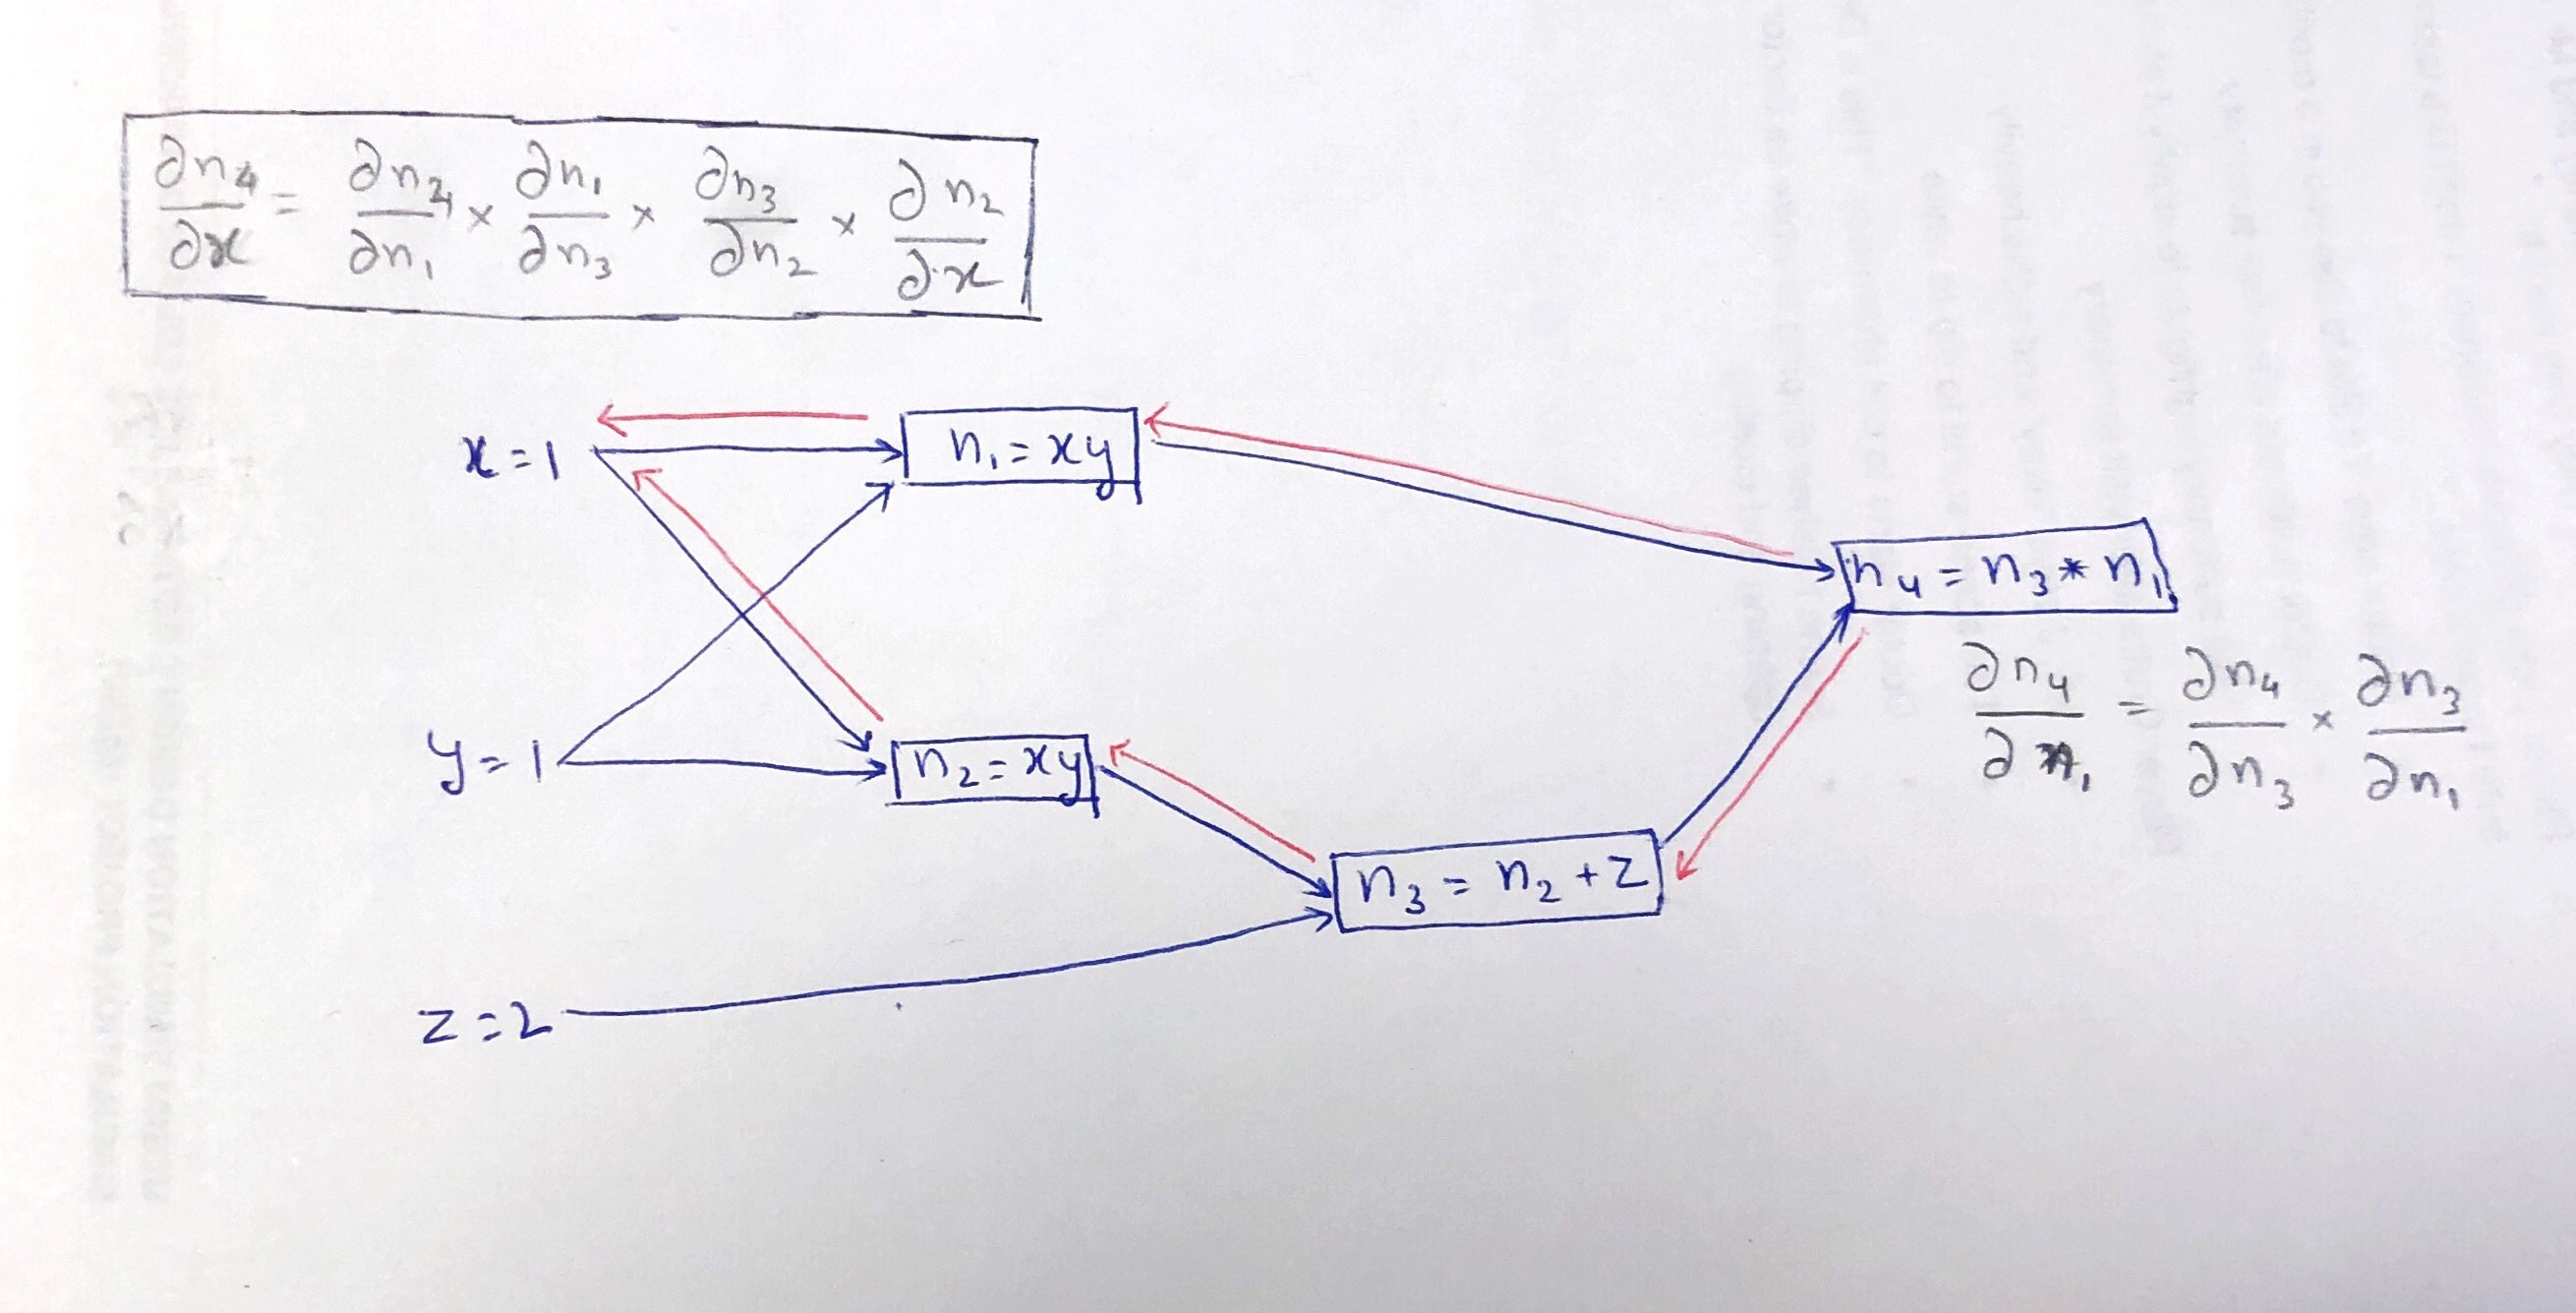
\includegraphics{ChainRule.jpeg}

    The partial derivative of computation graph w.r.t 'x' xan also be find
using mathematics: 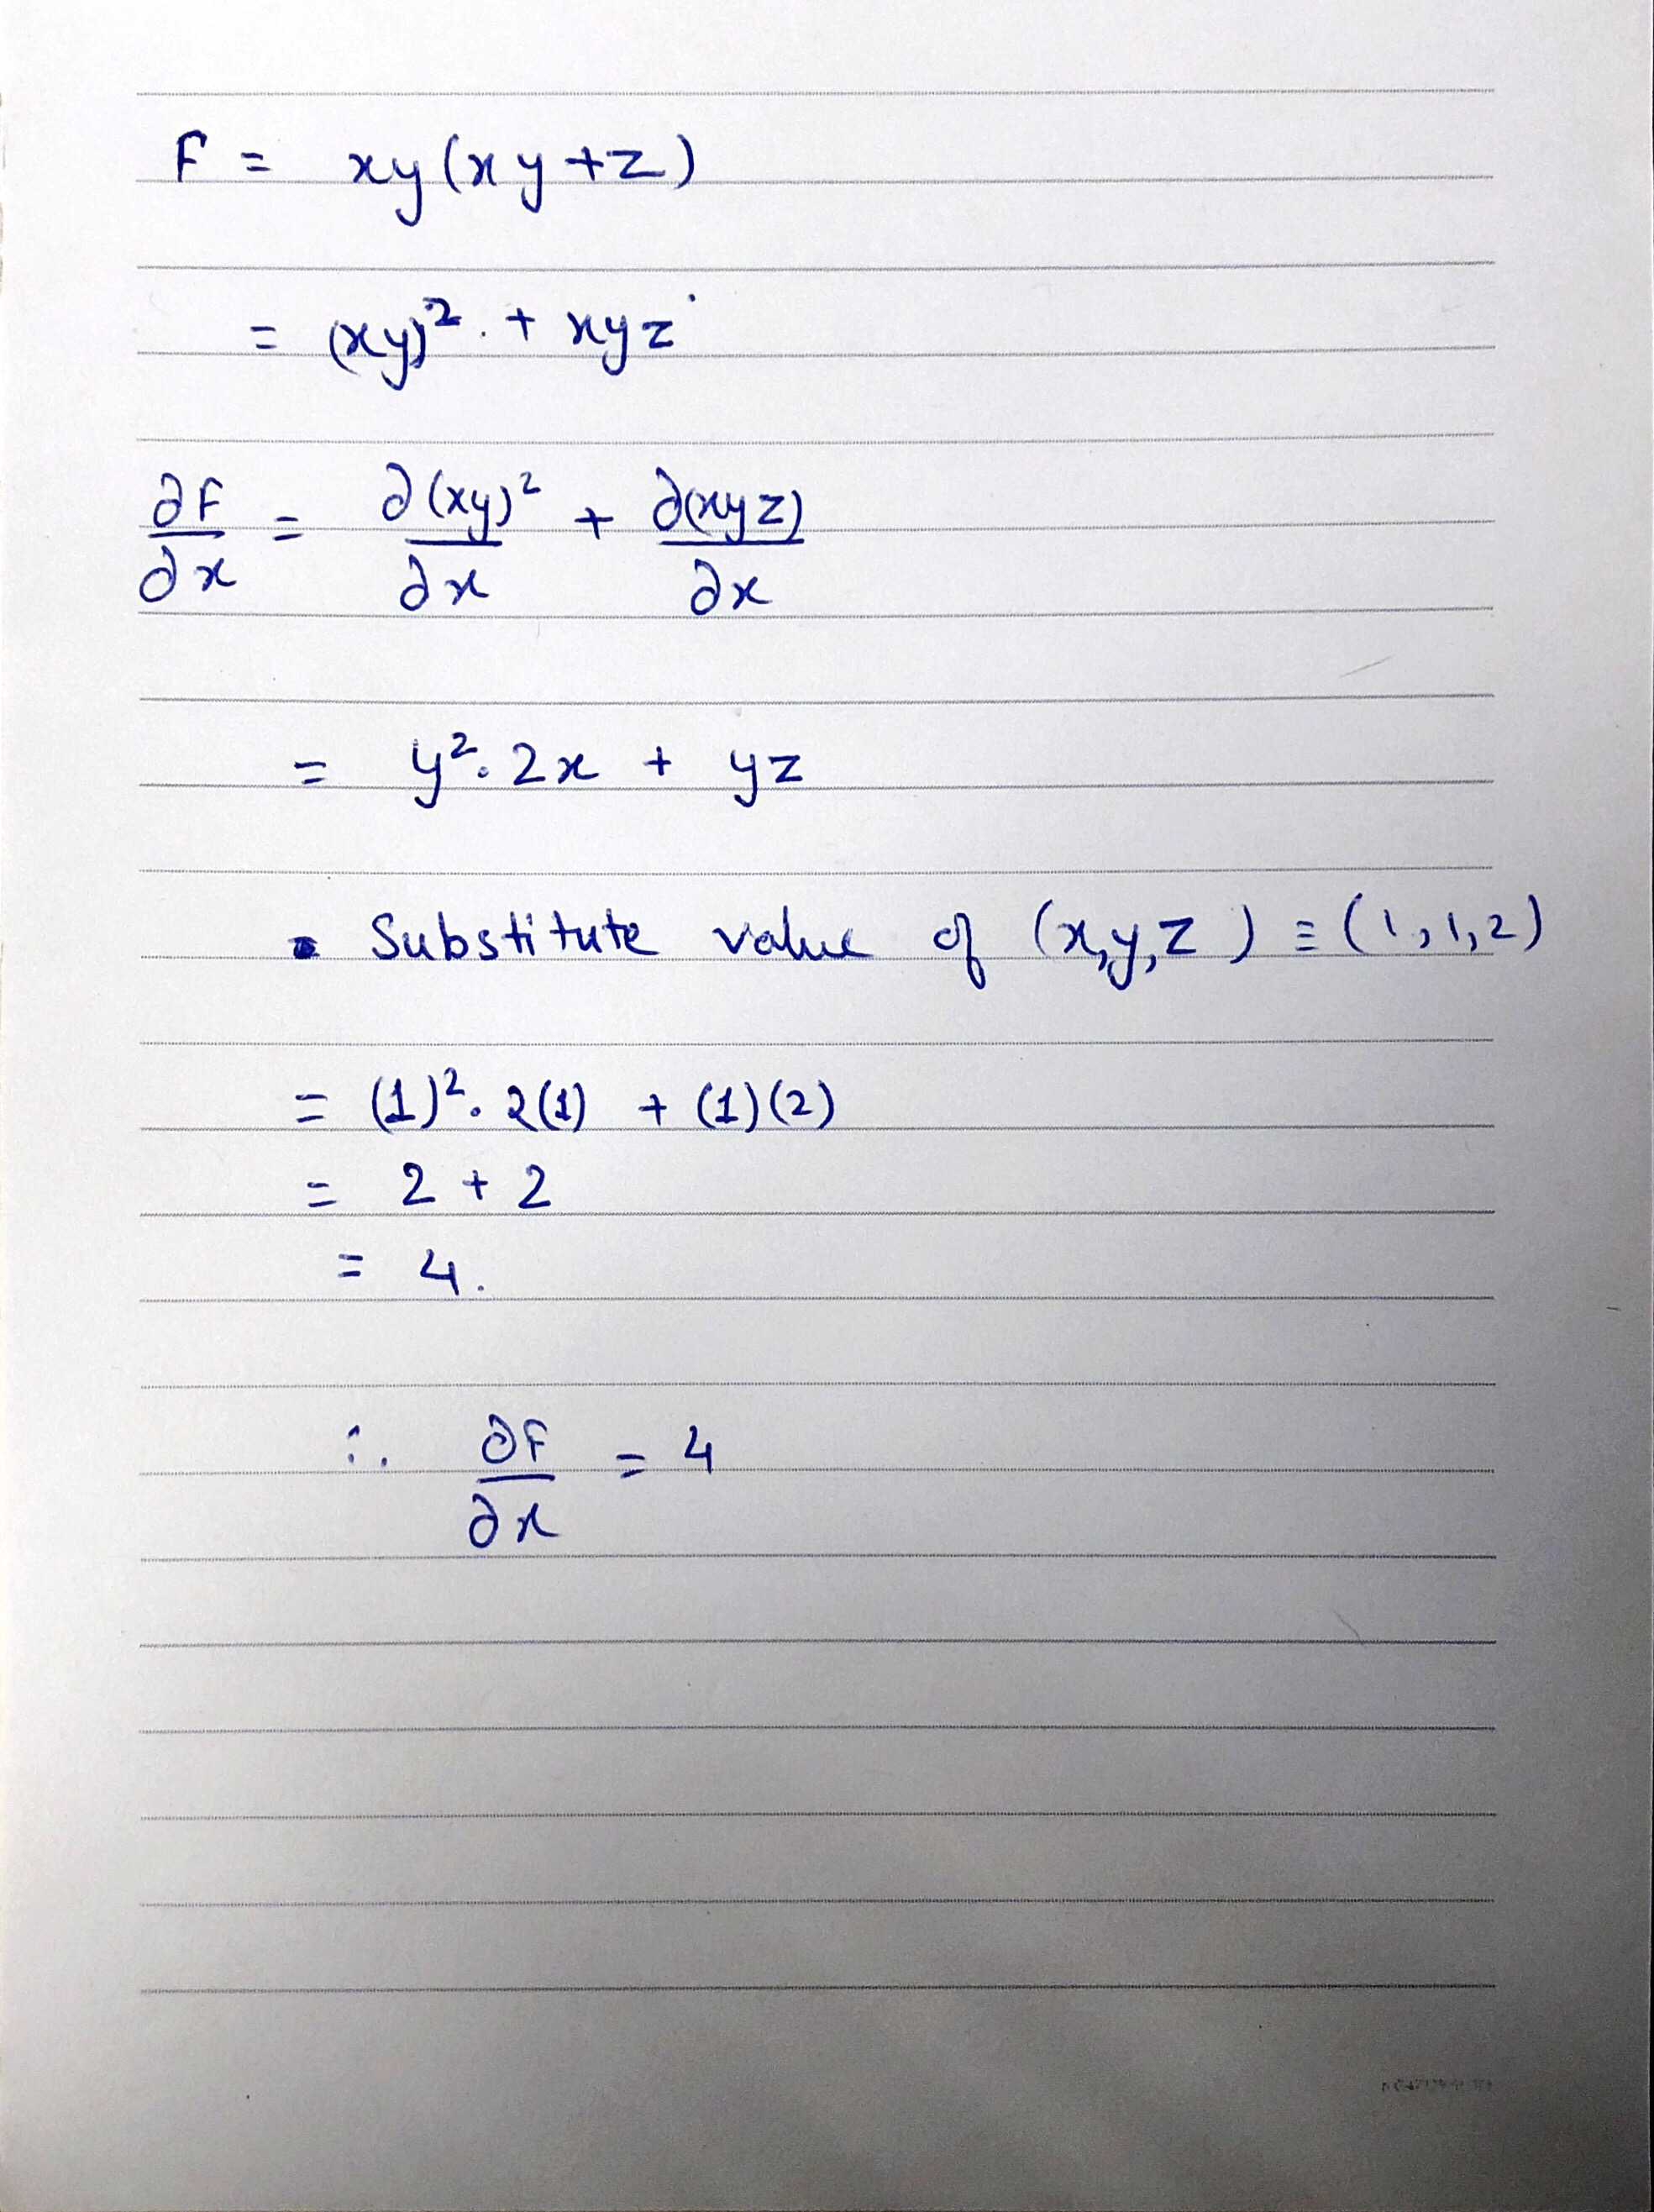
\includegraphics{Solution.jpeg}

    \begin{Verbatim}[commandchars=\\\{\}]
{\color{incolor}In [{\color{incolor}22}]:} \PY{c+c1}{\PYZsh{}\PYZsh{}\PYZsh{} Solution Ends here}
\end{Verbatim}


    \subsubsection{Problem 6:}\label{problem-6}

Multinomial Logistic Regression

\begin{itemize}
\item
  Using logistic regression predict classes by subsetting explanatory
  variable (shouldn't be all variables) with accuracy, precision and
  recall score and explain what you understood by scores
\item
  How would you avoid overfitting
\end{itemize}

    \begin{Verbatim}[commandchars=\\\{\}]
{\color{incolor}In [{\color{incolor}23}]:} \PY{n}{resp} \PY{o}{=} \PY{n}{urlopen}\PY{p}{(}\PY{l+s+s2}{\PYZdq{}}\PY{l+s+s2}{https://s3.amazonaws.com/aq\PYZhy{}web\PYZhy{}library/data.csv.zip}\PY{l+s+s2}{\PYZdq{}}\PY{p}{)}
         \PY{n}{zipfile\PYZus{}} \PY{o}{=} \PY{n}{ZipFile}\PY{p}{(}\PY{n}{BytesIO}\PY{p}{(}\PY{n}{resp}\PY{o}{.}\PY{n}{read}\PY{p}{(}\PY{p}{)}\PY{p}{)}\PY{p}{)}
         \PY{n}{df\PYZus{}log} \PY{o}{=} \PY{n}{pd}\PY{o}{.}\PY{n}{read\PYZus{}csv}\PY{p}{(}\PY{n}{zipfile\PYZus{}}\PY{o}{.}\PY{n}{open}\PY{p}{(}\PY{l+s+s1}{\PYZsq{}}\PY{l+s+s1}{data.csv}\PY{l+s+s1}{\PYZsq{}}\PY{p}{)}\PY{p}{)}
\end{Verbatim}


    \begin{Verbatim}[commandchars=\\\{\}]
{\color{incolor}In [{\color{incolor}24}]:} \PY{n}{df\PYZus{}log}\PY{o}{.}\PY{n}{head}\PY{p}{(}\PY{p}{)}
\end{Verbatim}


\begin{Verbatim}[commandchars=\\\{\}]
{\color{outcolor}Out[{\color{outcolor}24}]:}    class  alcohol  malic\_acid   ash  alcalinity  magnesium  total\_phenols  \textbackslash{}
         0      1    14.23        1.71  2.43        15.6        127           2.80   
         1      1    13.20        1.78  2.14        11.2        100           2.65   
         2      1    13.16        2.36  2.67        18.6        101           2.80   
         3      1    14.37        1.95  2.50        16.8        113           3.85   
         4      1    13.24        2.59  2.87        21.0        118           2.80   
         
            flavanoids  nonflavanoid\_phenols  proanthocyanins  color   hue    od  \textbackslash{}
         0        3.06                  0.28             2.29   5.64  1.04  3.92   
         1        2.76                  0.26             1.28   4.38  1.05  3.40   
         2        3.24                  0.30             2.81   5.68  1.03  3.17   
         3        3.49                  0.24             2.18   7.80  0.86  3.45   
         4        2.69                  0.39             1.82   4.32  1.04  2.93   
         
            proline  
         0     1065  
         1     1050  
         2     1185  
         3     1480  
         4      735  
\end{Verbatim}
            
    \begin{Verbatim}[commandchars=\\\{\}]
{\color{incolor}In [{\color{incolor}25}]:} \PY{n}{df\PYZus{}log}\PY{p}{[}\PY{l+s+s1}{\PYZsq{}}\PY{l+s+s1}{class}\PY{l+s+s1}{\PYZsq{}}\PY{p}{]}\PY{o}{.}\PY{n}{unique}\PY{p}{(}\PY{p}{)}
\end{Verbatim}


\begin{Verbatim}[commandchars=\\\{\}]
{\color{outcolor}Out[{\color{outcolor}25}]:} array([1, 2, 3], dtype=int64)
\end{Verbatim}
            
    \begin{Verbatim}[commandchars=\\\{\}]
{\color{incolor}In [{\color{incolor}26}]:} \PY{c+c1}{\PYZsh{}\PYZsh{}\PYZsh{} Solution for problem\PYZhy{}6 Starts Here}
         
         \PY{c+c1}{\PYZsh{} define X \PYZam{} Y as independent and dependent Variables respectively:}
         \PY{n}{X} \PY{o}{=} \PY{n}{df\PYZus{}log}\PY{o}{.}\PY{n}{iloc}\PY{p}{[}\PY{p}{:}\PY{p}{,}\PY{l+m+mi}{1}\PY{p}{:}\PY{p}{]}
         \PY{n}{Y} \PY{o}{=} \PY{n}{df\PYZus{}log}\PY{o}{.}\PY{n}{iloc}\PY{p}{[}\PY{p}{:}\PY{p}{,}\PY{l+m+mi}{0}\PY{p}{]}
         
         \PY{c+c1}{\PYZsh{} Create model object:}
         \PY{n}{mul\PYZus{}reg} \PY{o}{=} \PY{n}{sklearn}\PY{o}{.}\PY{n}{linear\PYZus{}model}\PY{o}{.}\PY{n}{LogisticRegression}\PY{p}{(}\PY{p}{)}
         
         \PY{c+c1}{\PYZsh{}  Split the dataset into train and test set:}
         \PY{n}{x\PYZus{}train}\PY{p}{,} \PY{n}{x\PYZus{}test}\PY{p}{,} \PY{n}{y\PYZus{}train}\PY{p}{,} \PY{n}{y\PYZus{}test} \PY{o}{=} \PY{n}{sklearn}\PY{o}{.}\PY{n}{model\PYZus{}selection}\PY{o}{.}\PY{n}{train\PYZus{}test\PYZus{}split}\PY{p}{(}\PY{n}{X}\PY{p}{,} \PY{n}{Y}\PY{p}{,} \PY{n}{test\PYZus{}size}\PY{o}{=}\PY{l+m+mf}{0.3}\PY{p}{,} \PY{n}{random\PYZus{}state}\PY{o}{=}\PY{l+m+mi}{42}\PY{p}{)}
         
         \PY{c+c1}{\PYZsh{} Fit the model:}
         \PY{n}{mul\PYZus{}reg\PYZus{}cl} \PY{o}{=} \PY{n}{mul\PYZus{}reg}\PY{o}{.}\PY{n}{fit}\PY{p}{(}\PY{n}{x\PYZus{}train}\PY{p}{,}\PY{n}{y\PYZus{}train}\PY{p}{)}
         
         \PY{c+c1}{\PYZsh{} Predict value of y for test\PYZhy{}set and store it in y\PYZhy{}pred variable:}
         \PY{n}{y\PYZus{}pred} \PY{o}{=} \PY{n}{mul\PYZus{}reg\PYZus{}cl}\PY{o}{.}\PY{n}{predict}\PY{p}{(}\PY{n}{x\PYZus{}test}\PY{p}{)}
         
         \PY{c+c1}{\PYZsh{} Obtain the report of your model:}
         \PY{n+nb}{print}\PY{p}{(}\PY{n}{sklearn}\PY{o}{.}\PY{n}{metrics}\PY{o}{.}\PY{n}{classification\PYZus{}report}\PY{p}{(}\PY{n}{y\PYZus{}pred}\PY{o}{=}\PY{n}{y\PYZus{}pred}\PY{p}{,} \PY{n}{y\PYZus{}true}\PY{o}{=} \PY{n}{y\PYZus{}test}\PY{p}{)}\PY{p}{)}
\end{Verbatim}


    \begin{Verbatim}[commandchars=\\\{\}]
             precision    recall  f1-score   support

          1       1.00      1.00      1.00        19
          2       1.00      1.00      1.00        21
          3       1.00      1.00      1.00        14

avg / total       1.00      1.00      1.00        54


    \end{Verbatim}

    \paragraph{As we can clearly see that model has been overfitted. Now we
will try to avoid the overfitting in the model. To do that we have
different
techniques:}\label{as-we-can-clearly-see-that-model-has-been-overfitted.-now-we-will-try-to-avoid-the-overfitting-in-the-model.-to-do-that-we-have-different-techniques}

    \begin{Verbatim}[commandchars=\\\{\}]
{\color{incolor}In [{\color{incolor}27}]:} \PY{c+c1}{\PYZsh{} Defining a function to select low variance features:}
         \PY{k}{def} \PY{n+nf}{variance\PYZus{}threshold\PYZus{}selector}\PY{p}{(}\PY{n}{data}\PY{p}{,} \PY{n}{threshold}\PY{o}{=}\PY{l+m+mf}{0.5}\PY{p}{)}\PY{p}{:}
             \PY{n}{selector} \PY{o}{=} \PY{n}{VarianceThreshold}\PY{p}{(}\PY{n}{threshold}\PY{p}{)}
             \PY{n}{selector}\PY{o}{.}\PY{n}{fit}\PY{p}{(}\PY{n}{data}\PY{p}{)}
             \PY{k}{return} \PY{n}{data}\PY{p}{[}\PY{n}{data}\PY{o}{.}\PY{n}{columns}\PY{p}{[}\PY{n}{selector}\PY{o}{.}\PY{n}{get\PYZus{}support}\PY{p}{(}\PY{n}{indices}\PY{o}{=}\PY{k+kc}{True}\PY{p}{)}\PY{p}{]}\PY{p}{]}
\end{Verbatim}


    \begin{Verbatim}[commandchars=\\\{\}]
{\color{incolor}In [{\color{incolor}28}]:} \PY{c+c1}{\PYZsh{} Selecting independent variables using the variance threshold function:}
         \PY{n}{X}\PY{o}{=}\PY{n}{variance\PYZus{}threshold\PYZus{}selector}\PY{p}{(}\PY{n}{X}\PY{p}{,}\PY{n}{threshold}\PY{o}{=}\PY{l+m+mf}{0.5}\PY{p}{)}
\end{Verbatim}


    \begin{Verbatim}[commandchars=\\\{\}]
{\color{incolor}In [{\color{incolor}29}]:} \PY{c+c1}{\PYZsh{} Split the dataset into train and test set:}
         \PY{n}{x\PYZus{}train}\PY{p}{,} \PY{n}{x\PYZus{}test}\PY{p}{,} \PY{n}{y\PYZus{}train}\PY{p}{,} \PY{n}{y\PYZus{}test}\PY{o}{=} \PY{n}{sklearn}\PY{o}{.}\PY{n}{model\PYZus{}selection}\PY{o}{.}\PY{n}{train\PYZus{}test\PYZus{}split}\PY{p}{(}\PY{n}{X}\PY{p}{,} \PY{n}{Y}\PY{p}{,} \PY{n}{test\PYZus{}size}\PY{o}{=}\PY{l+m+mf}{0.3}\PY{p}{,} \PY{n}{random\PYZus{}state}\PY{o}{=}\PY{l+m+mi}{42}\PY{p}{)}
         
         \PY{c+c1}{\PYZsh{} Fit the model:}
         \PY{n}{mul\PYZus{}reg\PYZus{}cl} \PY{o}{=} \PY{n}{mul\PYZus{}reg}\PY{o}{.}\PY{n}{fit}\PY{p}{(}\PY{n}{x\PYZus{}train}\PY{p}{,}\PY{n}{y\PYZus{}train}\PY{p}{)}
         
         \PY{c+c1}{\PYZsh{} Predict value of y for test\PYZhy{}set and store it in y\PYZhy{}pred variable:}
         \PY{n}{y\PYZus{}pred} \PY{o}{=} \PY{n}{mul\PYZus{}reg\PYZus{}cl}\PY{o}{.}\PY{n}{predict}\PY{p}{(}\PY{n}{x\PYZus{}test}\PY{p}{)}
         
         \PY{c+c1}{\PYZsh{} Obtain the report of your model:}
         \PY{n+nb}{print}\PY{p}{(}\PY{n}{sklearn}\PY{o}{.}\PY{n}{metrics}\PY{o}{.}\PY{n}{classification\PYZus{}report}\PY{p}{(}\PY{n}{y\PYZus{}pred}\PY{o}{=}\PY{n}{y\PYZus{}pred}\PY{p}{,} \PY{n}{y\PYZus{}true}\PY{o}{=} \PY{n}{y\PYZus{}test}\PY{p}{)}\PY{p}{)}
         
         \PY{c+c1}{\PYZsh{}\PYZsh{}\PYZsh{} Solution Ends Here}
\end{Verbatim}


    \begin{Verbatim}[commandchars=\\\{\}]
             precision    recall  f1-score   support

          1       0.95      1.00      0.97        19
          2       1.00      0.95      0.98        21
          3       1.00      1.00      1.00        14

avg / total       0.98      0.98      0.98        54


    \end{Verbatim}

    \section{Conclusion:}\label{conclusion}

\emph{There are various other techniques to avoid overfitting. Variance
Trade-off is one of the most popular Regularization methods used to
handle overfitting. Some other regularization methods are L1 and L2
regularization. Depending on the scenario, we can also increase the
dataset size or can use early stopping technique to avoid overfitting.}

    \subsubsection{Problem 7:}\label{problem-7}

\textbf{Problem}

Predict presence or absence of cardiovascular disease using the patient
examination results.

\textbf{Data description}

\begin{longtable}[]{@{}llll@{}}
\toprule
\begin{minipage}[b]{0.12\columnwidth}\raggedright\strut
Feature\strut
\end{minipage} & \begin{minipage}[b]{0.18\columnwidth}\raggedright\strut
Variable Type\strut
\end{minipage} & \begin{minipage}[b]{0.20\columnwidth}\raggedright\strut
Variable\strut
\end{minipage} & \begin{minipage}[b]{0.16\columnwidth}\raggedright\strut
Value Type\strut
\end{minipage}\tabularnewline
\midrule
\endhead
\begin{minipage}[t]{0.12\columnwidth}\raggedright\strut
Age\strut
\end{minipage} & \begin{minipage}[t]{0.18\columnwidth}\raggedright\strut
Objective Feature\strut
\end{minipage} & \begin{minipage}[t]{0.20\columnwidth}\raggedright\strut
age\strut
\end{minipage} & \begin{minipage}[t]{0.16\columnwidth}\raggedright\strut
int (days)\strut
\end{minipage}\tabularnewline
\begin{minipage}[t]{0.12\columnwidth}\raggedright\strut
Height\strut
\end{minipage} & \begin{minipage}[t]{0.18\columnwidth}\raggedright\strut
Objective Feature\strut
\end{minipage} & \begin{minipage}[t]{0.20\columnwidth}\raggedright\strut
height\strut
\end{minipage} & \begin{minipage}[t]{0.16\columnwidth}\raggedright\strut
int (cm)\strut
\end{minipage}\tabularnewline
\begin{minipage}[t]{0.12\columnwidth}\raggedright\strut
Weight\strut
\end{minipage} & \begin{minipage}[t]{0.18\columnwidth}\raggedright\strut
Objective Feature\strut
\end{minipage} & \begin{minipage}[t]{0.20\columnwidth}\raggedright\strut
weight\strut
\end{minipage} & \begin{minipage}[t]{0.16\columnwidth}\raggedright\strut
float (kg)\strut
\end{minipage}\tabularnewline
\begin{minipage}[t]{0.12\columnwidth}\raggedright\strut
Gender\strut
\end{minipage} & \begin{minipage}[t]{0.18\columnwidth}\raggedright\strut
Objective Feature\strut
\end{minipage} & \begin{minipage}[t]{0.20\columnwidth}\raggedright\strut
gender\strut
\end{minipage} & \begin{minipage}[t]{0.16\columnwidth}\raggedright\strut
categorical code\strut
\end{minipage}\tabularnewline
\begin{minipage}[t]{0.12\columnwidth}\raggedright\strut
Systolic blood pressure\strut
\end{minipage} & \begin{minipage}[t]{0.18\columnwidth}\raggedright\strut
Examination Feature\strut
\end{minipage} & \begin{minipage}[t]{0.20\columnwidth}\raggedright\strut
ap\_hi\strut
\end{minipage} & \begin{minipage}[t]{0.16\columnwidth}\raggedright\strut
int\strut
\end{minipage}\tabularnewline
\begin{minipage}[t]{0.12\columnwidth}\raggedright\strut
Diastolic blood pressure\strut
\end{minipage} & \begin{minipage}[t]{0.18\columnwidth}\raggedright\strut
Examination Feature\strut
\end{minipage} & \begin{minipage}[t]{0.20\columnwidth}\raggedright\strut
ap\_lo\strut
\end{minipage} & \begin{minipage}[t]{0.16\columnwidth}\raggedright\strut
int\strut
\end{minipage}\tabularnewline
\begin{minipage}[t]{0.12\columnwidth}\raggedright\strut
Cholesterol\strut
\end{minipage} & \begin{minipage}[t]{0.18\columnwidth}\raggedright\strut
Examination Feature\strut
\end{minipage} & \begin{minipage}[t]{0.20\columnwidth}\raggedright\strut
cholesterol\strut
\end{minipage} & \begin{minipage}[t]{0.16\columnwidth}\raggedright\strut
1: normal, 2: above normal, 3: well above normal\strut
\end{minipage}\tabularnewline
\begin{minipage}[t]{0.12\columnwidth}\raggedright\strut
Glucose\strut
\end{minipage} & \begin{minipage}[t]{0.18\columnwidth}\raggedright\strut
Examination Feature\strut
\end{minipage} & \begin{minipage}[t]{0.20\columnwidth}\raggedright\strut
gluc\strut
\end{minipage} & \begin{minipage}[t]{0.16\columnwidth}\raggedright\strut
1: normal, 2: above normal, 3: well above normal\strut
\end{minipage}\tabularnewline
\begin{minipage}[t]{0.12\columnwidth}\raggedright\strut
Smoking\strut
\end{minipage} & \begin{minipage}[t]{0.18\columnwidth}\raggedright\strut
Subjective Feature\strut
\end{minipage} & \begin{minipage}[t]{0.20\columnwidth}\raggedright\strut
smoke\strut
\end{minipage} & \begin{minipage}[t]{0.16\columnwidth}\raggedright\strut
binary\strut
\end{minipage}\tabularnewline
\begin{minipage}[t]{0.12\columnwidth}\raggedright\strut
Alcohol intake\strut
\end{minipage} & \begin{minipage}[t]{0.18\columnwidth}\raggedright\strut
Subjective Feature\strut
\end{minipage} & \begin{minipage}[t]{0.20\columnwidth}\raggedright\strut
alco\strut
\end{minipage} & \begin{minipage}[t]{0.16\columnwidth}\raggedright\strut
binary\strut
\end{minipage}\tabularnewline
\begin{minipage}[t]{0.12\columnwidth}\raggedright\strut
Physical activity\strut
\end{minipage} & \begin{minipage}[t]{0.18\columnwidth}\raggedright\strut
Subjective Feature\strut
\end{minipage} & \begin{minipage}[t]{0.20\columnwidth}\raggedright\strut
active\strut
\end{minipage} & \begin{minipage}[t]{0.16\columnwidth}\raggedright\strut
binary\strut
\end{minipage}\tabularnewline
\begin{minipage}[t]{0.12\columnwidth}\raggedright\strut
Presence or absence of cardiovascular disease\strut
\end{minipage} & \begin{minipage}[t]{0.18\columnwidth}\raggedright\strut
Target Variable\strut
\end{minipage} & \begin{minipage}[t]{0.20\columnwidth}\raggedright\strut
cardio\strut
\end{minipage} & \begin{minipage}[t]{0.16\columnwidth}\raggedright\strut
binary\strut
\end{minipage}\tabularnewline
\bottomrule
\end{longtable}

Task: * use dummy-encoding or One Hot Encoding (OHE), Feature
Engineering * Split data into train and holdout parts in the proportion
of 70\%/30\% using sklearn.model\_selection.train\_test\_split with
random\_state=1, into X\_train, X\_valid, y\_train, y\_valid

    \begin{Verbatim}[commandchars=\\\{\}]
{\color{incolor}In [{\color{incolor}30}]:} \PY{n}{resp} \PY{o}{=} \PY{n}{urlopen}\PY{p}{(}\PY{l+s+s2}{\PYZdq{}}\PY{l+s+s2}{https://s3.amazonaws.com/aq\PYZhy{}web\PYZhy{}library/data1.csv.zip}\PY{l+s+s2}{\PYZdq{}}\PY{p}{)}
         \PY{n}{zipfile\PYZus{}} \PY{o}{=} \PY{n}{ZipFile}\PY{p}{(}\PY{n}{BytesIO}\PY{p}{(}\PY{n}{resp}\PY{o}{.}\PY{n}{read}\PY{p}{(}\PY{p}{)}\PY{p}{)}\PY{p}{)}
         \PY{n}{df\PYZus{}dt} \PY{o}{=} \PY{n}{pd}\PY{o}{.}\PY{n}{read\PYZus{}csv}\PY{p}{(}\PY{n}{zipfile\PYZus{}}\PY{o}{.}\PY{n}{open}\PY{p}{(}\PY{l+s+s1}{\PYZsq{}}\PY{l+s+s1}{data1.csv}\PY{l+s+s1}{\PYZsq{}}\PY{p}{)}\PY{p}{,}\PY{n}{index\PYZus{}col}\PY{o}{=}\PY{l+s+s1}{\PYZsq{}}\PY{l+s+s1}{id}\PY{l+s+s1}{\PYZsq{}}\PY{p}{,} \PY{n}{sep}\PY{o}{=}\PY{l+s+s1}{\PYZsq{}}\PY{l+s+s1}{;}\PY{l+s+s1}{\PYZsq{}}\PY{p}{)}
\end{Verbatim}


    \begin{Verbatim}[commandchars=\\\{\}]
{\color{incolor}In [{\color{incolor}31}]:} \PY{n}{df\PYZus{}dt}\PY{o}{.}\PY{n}{head}\PY{p}{(}\PY{p}{)}
\end{Verbatim}


\begin{Verbatim}[commandchars=\\\{\}]
{\color{outcolor}Out[{\color{outcolor}31}]:}       age  gender  height  weight  ap\_hi  ap\_lo  cholesterol  gluc  smoke  \textbackslash{}
         id                                                                          
         0   18393       2     168    62.0    110     80            1     1      0   
         1   20228       1     156    85.0    140     90            3     1      0   
         2   18857       1     165    64.0    130     70            3     1      0   
         3   17623       2     169    82.0    150    100            1     1      0   
         4   17474       1     156    56.0    100     60            1     1      0   
         
             alco  active  cardio  
         id                        
         0      0       1       0  
         1      0       1       1  
         2      0       0       1  
         3      0       1       1  
         4      0       0       0  
\end{Verbatim}
            
    \textbf{Pre-processing on Data/Task:}

    \begin{Verbatim}[commandchars=\\\{\}]
{\color{incolor}In [{\color{incolor}32}]:} \PY{c+c1}{\PYZsh{} Converting age into categorical variables:}
         \PY{n}{age}\PY{o}{=}\PY{p}{[}\PY{p}{]}
         \PY{k}{for} \PY{n}{x} \PY{o+ow}{in} \PY{n}{df\PYZus{}dt}\PY{o}{.}\PY{n}{age}\PY{p}{:}
             
             \PY{k}{if} \PY{p}{(}\PY{n}{x}\PY{o}{/}\PY{l+m+mi}{365}\PY{p}{)}\PY{o}{\PYZlt{}}\PY{l+m+mi}{35}\PY{p}{:}
                 \PY{n}{age}\PY{o}{.}\PY{n}{append}\PY{p}{(}\PY{l+s+s1}{\PYZsq{}}\PY{l+s+s1}{Age[less\PYZus{}than\PYZus{}35]}\PY{l+s+s1}{\PYZsq{}}\PY{p}{)}
             
             \PY{k}{elif} \PY{p}{(}\PY{n}{x}\PY{o}{/}\PY{l+m+mi}{365}\PY{p}{)}\PY{o}{\PYZgt{}}\PY{o}{=}\PY{l+m+mi}{35} \PY{o+ow}{and} \PY{p}{(}\PY{n}{x}\PY{o}{/}\PY{l+m+mi}{365}\PY{p}{)}\PY{o}{\PYZlt{}}\PY{o}{=}\PY{l+m+mi}{45} \PY{p}{:}
                 \PY{n}{age}\PY{o}{.}\PY{n}{append}\PY{p}{(}\PY{l+s+s1}{\PYZsq{}}\PY{l+s+s1}{Age[35\PYZhy{}45]}\PY{l+s+s1}{\PYZsq{}}\PY{p}{)}
                 
             \PY{k}{elif} \PY{p}{(}\PY{n}{x}\PY{o}{/}\PY{l+m+mi}{365}\PY{p}{)}\PY{o}{\PYZgt{}}\PY{l+m+mi}{45} \PY{o+ow}{and} \PY{p}{(}\PY{n}{x}\PY{o}{/}\PY{l+m+mi}{365}\PY{p}{)}\PY{o}{\PYZlt{}}\PY{o}{=}\PY{l+m+mi}{55} \PY{p}{:}
                 \PY{n}{age}\PY{o}{.}\PY{n}{append}\PY{p}{(}\PY{l+s+s1}{\PYZsq{}}\PY{l+s+s1}{Age[46\PYZhy{}55]}\PY{l+s+s1}{\PYZsq{}}\PY{p}{)}
             
             \PY{k}{else}\PY{p}{:}
                 \PY{n}{age}\PY{o}{.}\PY{n}{append}\PY{p}{(}\PY{l+s+s1}{\PYZsq{}}\PY{l+s+s1}{Age[more than 55]}\PY{l+s+s1}{\PYZsq{}}\PY{p}{)}
         \PY{n}{df\PYZus{}dt}\PY{o}{.}\PY{n}{age}\PY{o}{=} \PY{n}{age}
         \PY{n}{res} \PY{o}{=} \PY{n}{pd}\PY{o}{.}\PY{n}{get\PYZus{}dummies}\PY{p}{(}\PY{n}{df\PYZus{}dt}\PY{o}{.}\PY{n}{age}\PY{p}{)}
         \PY{n}{df\PYZus{}dt}\PY{o}{=}\PY{n}{pd}\PY{o}{.}\PY{n}{concat}\PY{p}{(}\PY{p}{[}\PY{n}{df\PYZus{}dt}\PY{p}{,}\PY{n}{res}\PY{p}{]}\PY{p}{,}\PY{n}{axis}\PY{o}{=}\PY{l+m+mi}{1}\PY{p}{)}
         \PY{n}{df\PYZus{}dt}\PY{o}{=}\PY{n}{df\PYZus{}dt}\PY{o}{.}\PY{n}{drop}\PY{p}{(}\PY{n}{columns}\PY{o}{=}\PY{l+s+s1}{\PYZsq{}}\PY{l+s+s1}{age}\PY{l+s+s1}{\PYZsq{}}\PY{p}{)}
\end{Verbatim}


    \begin{Verbatim}[commandchars=\\\{\}]
{\color{incolor}In [{\color{incolor}33}]:} \PY{c+c1}{\PYZsh{} Converting Gender into categorical variables:}
         \PY{n}{gender}\PY{o}{=}\PY{p}{[}\PY{p}{]}
         \PY{k}{for} \PY{n}{x} \PY{o+ow}{in} \PY{n}{df\PYZus{}dt}\PY{o}{.}\PY{n}{gender}\PY{p}{:}
             \PY{k}{if} \PY{n}{x}\PY{o}{==}\PY{l+m+mi}{1}\PY{p}{:}
                 \PY{n}{gender}\PY{o}{.}\PY{n}{append}\PY{p}{(}\PY{l+m+mi}{0}\PY{p}{)}
             \PY{k}{else}\PY{p}{:}
                 \PY{n}{gender}\PY{o}{.}\PY{n}{append}\PY{p}{(}\PY{l+m+mi}{1}\PY{p}{)}
         
         \PY{n}{df\PYZus{}dt}\PY{p}{[}\PY{l+s+s1}{\PYZsq{}}\PY{l+s+s1}{gender}\PY{l+s+s1}{\PYZsq{}}\PY{p}{]}\PY{o}{=}\PY{n}{gender}
\end{Verbatim}


    \begin{Verbatim}[commandchars=\\\{\}]
{\color{incolor}In [{\color{incolor}34}]:} \PY{c+c1}{\PYZsh{} Converting height into categorical variables:}
         \PY{n}{height}\PY{o}{=}\PY{p}{[}\PY{p}{]}
         \PY{k}{for} \PY{n}{x} \PY{o+ow}{in} \PY{n}{df\PYZus{}dt}\PY{o}{.}\PY{n}{height}\PY{p}{:}
             \PY{k}{if} \PY{n}{x}\PY{o}{\PYZlt{}}\PY{l+m+mi}{100}\PY{p}{:}
                 \PY{n}{height}\PY{o}{.}\PY{n}{append}\PY{p}{(}\PY{l+s+s1}{\PYZsq{}}\PY{l+s+s1}{Height[Less\PYZus{}than\PYZus{}100]}\PY{l+s+s1}{\PYZsq{}}\PY{p}{)}
             \PY{k}{elif}  \PY{n}{x}\PY{o}{\PYZgt{}}\PY{o}{=}\PY{l+m+mi}{100} \PY{o+ow}{and} \PY{n}{x}\PY{o}{\PYZlt{}}\PY{o}{=}\PY{l+m+mi}{150}\PY{p}{:}
                 \PY{n}{height}\PY{o}{.}\PY{n}{append}\PY{p}{(}\PY{l+s+s1}{\PYZsq{}}\PY{l+s+s1}{Height[100\PYZhy{}150]}\PY{l+s+s1}{\PYZsq{}}\PY{p}{)}
             \PY{k}{elif}  \PY{n}{x}\PY{o}{\PYZgt{}}\PY{l+m+mi}{150} \PY{o+ow}{and} \PY{n}{x}\PY{o}{\PYZlt{}}\PY{o}{=}\PY{l+m+mi}{200}\PY{p}{:}
                 \PY{n}{height}\PY{o}{.}\PY{n}{append}\PY{p}{(}\PY{l+s+s1}{\PYZsq{}}\PY{l+s+s1}{Height[151\PYZhy{}200]}\PY{l+s+s1}{\PYZsq{}}\PY{p}{)}
             \PY{k}{else}\PY{p}{:}
                 \PY{n}{height}\PY{o}{.}\PY{n}{append}\PY{p}{(}\PY{l+s+s1}{\PYZsq{}}\PY{l+s+s1}{Height[More\PYZus{}than\PYZus{}200]}\PY{l+s+s1}{\PYZsq{}}\PY{p}{)}
         
         \PY{n}{df\PYZus{}dt}\PY{p}{[}\PY{l+s+s1}{\PYZsq{}}\PY{l+s+s1}{height}\PY{l+s+s1}{\PYZsq{}}\PY{p}{]}\PY{o}{=} \PY{n}{height}
         
         \PY{n}{res1} \PY{o}{=} \PY{n}{pd}\PY{o}{.}\PY{n}{get\PYZus{}dummies}\PY{p}{(}\PY{n}{df\PYZus{}dt}\PY{o}{.}\PY{n}{height}\PY{p}{)}
         
         \PY{n}{df\PYZus{}dt}\PY{o}{=}\PY{n}{pd}\PY{o}{.}\PY{n}{concat}\PY{p}{(}\PY{p}{[}\PY{n}{df\PYZus{}dt}\PY{p}{,}\PY{n}{res1}\PY{p}{]}\PY{p}{,}\PY{n}{axis}\PY{o}{=}\PY{l+m+mi}{1}\PY{p}{)}
         
         \PY{n}{df\PYZus{}dt}\PY{o}{=}\PY{n}{df\PYZus{}dt}\PY{o}{.}\PY{n}{drop}\PY{p}{(}\PY{n}{columns}\PY{o}{=}\PY{l+s+s1}{\PYZsq{}}\PY{l+s+s1}{height}\PY{l+s+s1}{\PYZsq{}}\PY{p}{)}
\end{Verbatim}


    \begin{Verbatim}[commandchars=\\\{\}]
{\color{incolor}In [{\color{incolor}35}]:} \PY{c+c1}{\PYZsh{} Before converting weight into categorical variables, we will try to depict variance:}
         \PY{n}{plt}\PY{o}{.}\PY{n}{scatter}\PY{p}{(}\PY{n}{df\PYZus{}dt}\PY{o}{.}\PY{n}{weight}\PY{p}{,}\PY{n+nb}{range}\PY{p}{(}\PY{n+nb}{len}\PY{p}{(}\PY{n}{df\PYZus{}dt}\PY{o}{.}\PY{n}{weight}\PY{p}{)}\PY{p}{)}\PY{p}{)}
\end{Verbatim}


\begin{Verbatim}[commandchars=\\\{\}]
{\color{outcolor}Out[{\color{outcolor}35}]:} <matplotlib.collections.PathCollection at 0x214e24e14a8>
\end{Verbatim}
            
    \begin{center}
    \adjustimage{max size={0.9\linewidth}{0.9\paperheight}}{output_48_1.png}
    \end{center}
    { \hspace*{\fill} \\}
    
    \begin{Verbatim}[commandchars=\\\{\}]
{\color{incolor}In [{\color{incolor}36}]:} \PY{c+c1}{\PYZsh{} Converting weight into categorical variables:}
         \PY{n}{weight}\PY{o}{=}\PY{p}{[}\PY{p}{]}
         \PY{k}{for} \PY{n}{x} \PY{o+ow}{in} \PY{n}{df\PYZus{}dt}\PY{o}{.}\PY{n}{weight}\PY{p}{:}
             \PY{k}{if} \PY{n}{x} \PY{o}{\PYZlt{}}\PY{l+m+mi}{50}\PY{p}{:}
                 \PY{n}{weight}\PY{o}{.}\PY{n}{append}\PY{p}{(}\PY{l+s+s1}{\PYZsq{}}\PY{l+s+s1}{Weigth[Less\PYZus{}than\PYZus{}50]}\PY{l+s+s1}{\PYZsq{}}\PY{p}{)}
             \PY{k}{elif} \PY{n}{x}\PY{o}{\PYZgt{}}\PY{o}{=}\PY{l+m+mi}{50} \PY{o+ow}{and} \PY{n}{x}\PY{o}{\PYZlt{}}\PY{o}{=}\PY{l+m+mi}{75}\PY{p}{:}
                 \PY{n}{weight}\PY{o}{.}\PY{n}{append}\PY{p}{(}\PY{l+s+s1}{\PYZsq{}}\PY{l+s+s1}{weight[50\PYZhy{}75]}\PY{l+s+s1}{\PYZsq{}}\PY{p}{)}
             \PY{k}{elif} \PY{n}{x}\PY{o}{\PYZgt{}}\PY{l+m+mi}{75} \PY{o+ow}{and} \PY{n}{x}\PY{o}{\PYZlt{}}\PY{o}{=}\PY{l+m+mi}{100}\PY{p}{:}
                 \PY{n}{weight}\PY{o}{.}\PY{n}{append}\PY{p}{(}\PY{l+s+s1}{\PYZsq{}}\PY{l+s+s1}{weight[76\PYZhy{}100]}\PY{l+s+s1}{\PYZsq{}}\PY{p}{)}
             \PY{k}{elif} \PY{n}{x}\PY{o}{\PYZgt{}}\PY{l+m+mi}{100} \PY{o+ow}{and} \PY{n}{x}\PY{o}{\PYZlt{}}\PY{o}{=}\PY{l+m+mi}{125}\PY{p}{:}
                 \PY{n}{weight}\PY{o}{.}\PY{n}{append}\PY{p}{(}\PY{l+s+s1}{\PYZsq{}}\PY{l+s+s1}{weight[101\PYZhy{}125]}\PY{l+s+s1}{\PYZsq{}}\PY{p}{)}
             \PY{k}{else}\PY{p}{:}
                 \PY{n}{weight}\PY{o}{.}\PY{n}{append}\PY{p}{(}\PY{l+s+s1}{\PYZsq{}}\PY{l+s+s1}{weight[More\PYZus{}than\PYZus{}125]}\PY{l+s+s1}{\PYZsq{}}\PY{p}{)}
         
         \PY{n}{df\PYZus{}dt}\PY{p}{[}\PY{l+s+s1}{\PYZsq{}}\PY{l+s+s1}{weight}\PY{l+s+s1}{\PYZsq{}}\PY{p}{]}\PY{o}{=}\PY{n}{weight}
         
         \PY{n}{res4} \PY{o}{=} \PY{n}{pd}\PY{o}{.}\PY{n}{get\PYZus{}dummies}\PY{p}{(}\PY{n}{df\PYZus{}dt}\PY{o}{.}\PY{n}{weight}\PY{p}{)}
         
         \PY{n}{df\PYZus{}dt}\PY{o}{=}\PY{n}{pd}\PY{o}{.}\PY{n}{concat}\PY{p}{(}\PY{p}{[}\PY{n}{df\PYZus{}dt}\PY{p}{,}\PY{n}{res4}\PY{p}{]}\PY{p}{,}\PY{n}{axis}\PY{o}{=}\PY{l+m+mi}{1}\PY{p}{)}
         
         \PY{n}{df\PYZus{}dt}\PY{o}{=}\PY{n}{df\PYZus{}dt}\PY{o}{.}\PY{n}{drop}\PY{p}{(}\PY{n}{columns}\PY{o}{=}\PY{l+s+s1}{\PYZsq{}}\PY{l+s+s1}{weight}\PY{l+s+s1}{\PYZsq{}}\PY{p}{)}
\end{Verbatim}


    \subsubsection{Before converting 'ap\_hi' and 'ap\_lo' into categorical
variables, refer this
image:}\label{before-converting-ap_hi-and-ap_lo-into-categorical-variables-refer-this-image}

\begin{figure}
\centering
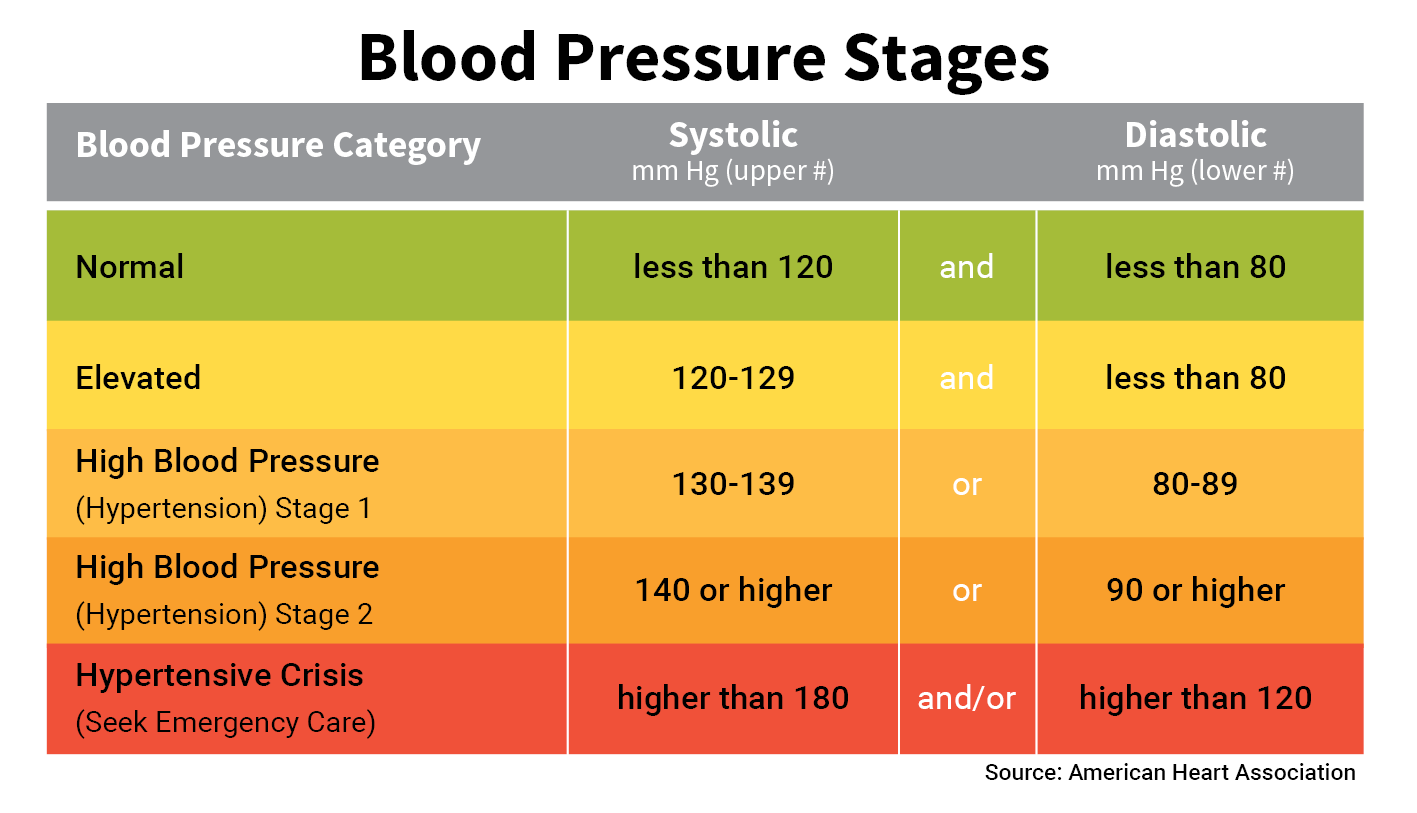
\includegraphics{basic_blood_pressure_chart.png}
\caption{title}
\end{figure}

\subsubsection{Instead of converting 'ap\_hi' and 'ap\_lo' into
categorical variables individually, using this image we created
categorical ranges of blood pressure which include both high and low
blood
pressure.}\label{instead-of-converting-ap_hi-and-ap_lo-into-categorical-variables-individually-using-this-image-we-created-categorical-ranges-of-blood-pressure-which-include-both-high-and-low-blood-pressure.}

    \begin{Verbatim}[commandchars=\\\{\}]
{\color{incolor}In [{\color{incolor}37}]:}   
         \PY{c+c1}{\PYZsh{} Converting Blood Pressure into categorical variables:}
         \PY{n}{blood\PYZus{}pressure}\PY{o}{=}\PY{p}{[}\PY{p}{]}
         \PY{k}{for} \PY{n}{x}\PY{p}{,}\PY{n}{y} \PY{o+ow}{in} \PY{n+nb}{zip}\PY{p}{(}\PY{n}{df\PYZus{}dt}\PY{o}{.}\PY{n}{ap\PYZus{}hi}\PY{p}{,}\PY{n}{df\PYZus{}dt}\PY{o}{.}\PY{n}{ap\PYZus{}lo}\PY{p}{)}\PY{p}{:}
             \PY{k}{if} \PY{n}{x}\PY{o}{\PYZlt{}}\PY{l+m+mi}{120} \PY{o+ow}{and} \PY{n}{y}\PY{o}{\PYZlt{}}\PY{l+m+mi}{80}\PY{p}{:}
                 \PY{n}{blood\PYZus{}pressure}\PY{o}{.}\PY{n}{append}\PY{p}{(}\PY{l+s+s1}{\PYZsq{}}\PY{l+s+s1}{BP\PYZhy{}Normal}\PY{l+s+s1}{\PYZsq{}}\PY{p}{)}
             \PY{k}{elif} \PY{p}{(}\PY{n}{x}\PY{o}{\PYZgt{}}\PY{o}{=}\PY{l+m+mi}{120} \PY{o+ow}{and} \PY{n}{x}\PY{o}{\PYZlt{}}\PY{o}{=}\PY{l+m+mi}{129}\PY{p}{)} \PY{o+ow}{and} \PY{n}{y}\PY{o}{\PYZlt{}}\PY{l+m+mi}{80}\PY{p}{:}
                 \PY{n}{blood\PYZus{}pressure}\PY{o}{.}\PY{n}{append}\PY{p}{(}\PY{l+s+s1}{\PYZsq{}}\PY{l+s+s1}{BP\PYZhy{}Elevated}\PY{l+s+s1}{\PYZsq{}}\PY{p}{)}
             \PY{k}{elif} \PY{p}{(}\PY{n}{x}\PY{o}{\PYZgt{}}\PY{o}{=}\PY{l+m+mi}{130} \PY{o+ow}{and} \PY{n}{x}\PY{o}{\PYZlt{}}\PY{o}{=}\PY{l+m+mi}{180}\PY{p}{)} \PY{o+ow}{or} \PY{p}{(}\PY{n}{y}\PY{o}{\PYZgt{}}\PY{o}{=}\PY{l+m+mi}{80} \PY{o+ow}{and} \PY{n}{y}\PY{o}{\PYZlt{}}\PY{o}{=}\PY{l+m+mi}{120}\PY{p}{)}\PY{p}{:}
                 \PY{n}{blood\PYZus{}pressure}\PY{o}{.}\PY{n}{append}\PY{p}{(}\PY{l+s+s1}{\PYZsq{}}\PY{l+s+s1}{BP\PYZhy{}High BP}\PY{l+s+s1}{\PYZsq{}}\PY{p}{)}
             \PY{k}{else}\PY{p}{:}
                 \PY{n}{blood\PYZus{}pressure}\PY{o}{.}\PY{n}{append}\PY{p}{(}\PY{l+s+s1}{\PYZsq{}}\PY{l+s+s1}{BP\PYZhy{}Hypertensive Crisis}\PY{l+s+s1}{\PYZsq{}}\PY{p}{)}
                 
         
         \PY{n}{df\PYZus{}dt}\PY{p}{[}\PY{l+s+s1}{\PYZsq{}}\PY{l+s+s1}{Blood\PYZus{}Pressure}\PY{l+s+s1}{\PYZsq{}}\PY{p}{]}\PY{o}{=} \PY{n}{blood\PYZus{}pressure}
         
         \PY{n}{df\PYZus{}dt}\PY{o}{=}\PY{n}{df\PYZus{}dt}\PY{o}{.}\PY{n}{drop}\PY{p}{(}\PY{n}{columns}\PY{o}{=}\PY{p}{[}\PY{l+s+s1}{\PYZsq{}}\PY{l+s+s1}{ap\PYZus{}hi}\PY{l+s+s1}{\PYZsq{}}\PY{p}{,}\PY{l+s+s1}{\PYZsq{}}\PY{l+s+s1}{ap\PYZus{}lo}\PY{l+s+s1}{\PYZsq{}}\PY{p}{]}\PY{p}{)}
         
         \PY{n}{res5} \PY{o}{=} \PY{n}{pd}\PY{o}{.}\PY{n}{get\PYZus{}dummies}\PY{p}{(}\PY{n}{df\PYZus{}dt}\PY{o}{.}\PY{n}{Blood\PYZus{}Pressure}\PY{p}{)}
         
         \PY{n}{df\PYZus{}dt}\PY{o}{=}\PY{n}{pd}\PY{o}{.}\PY{n}{concat}\PY{p}{(}\PY{p}{[}\PY{n}{df\PYZus{}dt}\PY{p}{,}\PY{n}{res5}\PY{p}{]}\PY{p}{,}\PY{n}{axis}\PY{o}{=}\PY{l+m+mi}{1}\PY{p}{)}
         
         \PY{n}{df\PYZus{}dt}\PY{o}{=}\PY{n}{df\PYZus{}dt}\PY{o}{.}\PY{n}{drop}\PY{p}{(}\PY{n}{columns}\PY{o}{=}\PY{l+s+s1}{\PYZsq{}}\PY{l+s+s1}{Blood\PYZus{}Pressure}\PY{l+s+s1}{\PYZsq{}}\PY{p}{)}
\end{Verbatim}


    \begin{Verbatim}[commandchars=\\\{\}]
{\color{incolor}In [{\color{incolor}38}]:} \PY{c+c1}{\PYZsh{} Defining Independent and dependent variables:}
         \PY{n}{X}\PY{o}{=} \PY{n}{df\PYZus{}dt}\PY{o}{.}\PY{n}{drop}\PY{p}{(}\PY{n}{columns}\PY{o}{=}\PY{l+s+s1}{\PYZsq{}}\PY{l+s+s1}{cardio}\PY{l+s+s1}{\PYZsq{}}\PY{p}{)} 
         \PY{n}{Y}\PY{o}{=} \PY{n}{df\PYZus{}dt}\PY{p}{[}\PY{l+s+s1}{\PYZsq{}}\PY{l+s+s1}{cardio}\PY{l+s+s1}{\PYZsq{}}\PY{p}{]}
\end{Verbatim}


    \begin{Verbatim}[commandchars=\\\{\}]
{\color{incolor}In [{\color{incolor}39}]:} \PY{c+c1}{\PYZsh{} Split the dataset into train and test dataset:}
         \PY{n}{x\PYZus{}train}\PY{p}{,} \PY{n}{x\PYZus{}test}\PY{p}{,} \PY{n}{y\PYZus{}train}\PY{p}{,} \PY{n}{y\PYZus{}test}\PY{o}{=} \PY{n}{sklearn}\PY{o}{.}\PY{n}{model\PYZus{}selection}\PY{o}{.}\PY{n}{train\PYZus{}test\PYZus{}split}\PY{p}{(}\PY{n}{X}\PY{p}{,}\PY{n}{Y}\PY{p}{,}\PY{n}{random\PYZus{}state}\PY{o}{=}\PY{l+m+mi}{1}\PY{p}{,} \PY{n}{train\PYZus{}size}\PY{o}{=}\PY{l+m+mf}{0.7}\PY{p}{,} \PY{n}{test\PYZus{}size}\PY{o}{=}\PY{l+m+mf}{0.3} \PY{p}{)}
\end{Verbatim}


    \paragraph{7.1}\label{section}

Train the decision tree on the dataset (X\_train, y\_train) with max
depth equals to 3 and random\_state=20. * What 3 features are used to
make predictions in the created decision tree? Calculate accuracy.

    \begin{Verbatim}[commandchars=\\\{\}]
{\color{incolor}In [{\color{incolor}40}]:} \PY{c+c1}{\PYZsh{}\PYZsh{}\PYZsh{} Solution for problem\PYZhy{}7.1 Starts Here}
         
         \PY{c+c1}{\PYZsh{} Training a Decision Tree:}
         
         \PY{n}{decision\PYZus{}tree}\PY{o}{=} \PY{n}{sklearn}\PY{o}{.}\PY{n}{tree}\PY{o}{.}\PY{n}{DecisionTreeClassifier}\PY{p}{(}\PY{n}{random\PYZus{}state}\PY{o}{=}\PY{l+m+mi}{20}\PY{p}{,}\PY{n}{max\PYZus{}depth}\PY{o}{=}\PY{l+m+mi}{3}\PY{p}{)}
         \PY{n}{model1}\PY{o}{=} \PY{n}{decision\PYZus{}tree}\PY{o}{.}\PY{n}{fit}\PY{p}{(}\PY{n}{x\PYZus{}train}\PY{p}{,}\PY{n}{y\PYZus{}train}\PY{p}{)}
         \PY{n}{model1}
\end{Verbatim}


\begin{Verbatim}[commandchars=\\\{\}]
{\color{outcolor}Out[{\color{outcolor}40}]:} DecisionTreeClassifier(class\_weight=None, criterion='gini', max\_depth=3,
                     max\_features=None, max\_leaf\_nodes=None,
                     min\_impurity\_decrease=0.0, min\_impurity\_split=None,
                     min\_samples\_leaf=1, min\_samples\_split=2,
                     min\_weight\_fraction\_leaf=0.0, presort=False, random\_state=20,
                     splitter='best')
\end{Verbatim}
            
    \begin{Verbatim}[commandchars=\\\{\}]
{\color{incolor}In [{\color{incolor}41}]:} \PY{c+c1}{\PYZsh{} To render the Decision Tree we will import few libraries:}
         
         \PY{k+kn}{from} \PY{n+nn}{sklearn}\PY{n+nn}{.}\PY{n+nn}{externals}\PY{n+nn}{.}\PY{n+nn}{six} \PY{k}{import} \PY{n}{StringIO}  
         \PY{k+kn}{from} \PY{n+nn}{IPython}\PY{n+nn}{.}\PY{n+nn}{display} \PY{k}{import} \PY{n}{Image}
         \PY{k+kn}{from} \PY{n+nn}{sklearn}\PY{n+nn}{.}\PY{n+nn}{tree} \PY{k}{import} \PY{n}{export\PYZus{}graphviz}
         \PY{k+kn}{import} \PY{n+nn}{pydotplus}
\end{Verbatim}


    \begin{Verbatim}[commandchars=\\\{\}]
{\color{incolor}In [{\color{incolor}42}]:} \PY{c+c1}{\PYZsh{} Rendering Decision tree:}
         
         \PY{n}{dot\PYZus{}data} \PY{o}{=} \PY{n}{StringIO}\PY{p}{(}\PY{p}{)}
         \PY{n}{export\PYZus{}graphviz}\PY{p}{(}\PY{n}{model1}\PY{p}{,} \PY{n}{out\PYZus{}file}\PY{o}{=}\PY{n}{dot\PYZus{}data}\PY{p}{,}  
                         \PY{n}{filled}\PY{o}{=}\PY{k+kc}{True}\PY{p}{,} \PY{n}{rounded}\PY{o}{=}\PY{k+kc}{True}\PY{p}{,}
                         \PY{n}{special\PYZus{}characters}\PY{o}{=}\PY{k+kc}{True}\PY{p}{,}\PY{n}{feature\PYZus{}names}\PY{o}{=}\PY{n+nb}{list}\PY{p}{(}\PY{n}{x\PYZus{}train}\PY{o}{.}\PY{n}{columns}\PY{p}{)}\PY{p}{)}
         \PY{n}{graph} \PY{o}{=} \PY{n}{pydotplus}\PY{o}{.}\PY{n}{graph\PYZus{}from\PYZus{}dot\PYZus{}data}\PY{p}{(}\PY{n}{dot\PYZus{}data}\PY{o}{.}\PY{n}{getvalue}\PY{p}{(}\PY{p}{)}\PY{p}{)}  
         \PY{n}{Image}\PY{p}{(}\PY{n}{graph}\PY{o}{.}\PY{n}{create\PYZus{}jpeg}\PY{p}{(}\PY{p}{)}\PY{p}{)}
\end{Verbatim}

\texttt{\color{outcolor}Out[{\color{outcolor}42}]:}
    
    \begin{center}
    \adjustimage{max size={0.9\linewidth}{0.9\paperheight}}{output_57_0.jpeg}
    \end{center}
    { \hspace*{\fill} \\}
    

    We can determine the 3 features primarily used to make predictions in
the created decision tree by seeing at decision tree: 1. BP-High BP 2.
Cholestrol 3. Age

To support this result we can also calculate feature ranking.

    \begin{Verbatim}[commandchars=\\\{\}]
{\color{incolor}In [{\color{incolor}43}]:} \PY{c+c1}{\PYZsh{} Calculate Feature Ranking:}
         \PY{n}{importances} \PY{o}{=} \PY{n}{model1}\PY{o}{.}\PY{n}{feature\PYZus{}importances\PYZus{}}
         \PY{n}{indices} \PY{o}{=} \PY{n}{np}\PY{o}{.}\PY{n}{argsort}\PY{p}{(}\PY{n}{importances}\PY{p}{)}\PY{p}{[}\PY{p}{:}\PY{p}{:}\PY{o}{\PYZhy{}}\PY{l+m+mi}{1}\PY{p}{]}
         
         \PY{c+c1}{\PYZsh{} Print the feature ranking}
         \PY{n+nb}{print}\PY{p}{(}\PY{l+s+s2}{\PYZdq{}}\PY{l+s+s2}{Feature ranking:}\PY{l+s+s2}{\PYZdq{}}\PY{p}{)}
         
         \PY{k}{for} \PY{n}{f} \PY{o+ow}{in} \PY{n+nb}{range}\PY{p}{(}\PY{n+nb}{len}\PY{p}{(}\PY{n}{x\PYZus{}test}\PY{o}{.}\PY{n}{columns}\PY{p}{)}\PY{p}{)}\PY{p}{:}
             \PY{n+nb}{print}\PY{p}{(}\PY{n}{f}\PY{o}{+}\PY{l+m+mi}{1}\PY{p}{,}\PY{n}{x\PYZus{}test}\PY{o}{.}\PY{n}{columns}\PY{p}{[}\PY{n}{indices}\PY{p}{[}\PY{n}{f}\PY{p}{]}\PY{p}{]}\PY{p}{,}\PY{l+s+s2}{\PYZdq{}}\PY{l+s+s2}{: }\PY{l+s+s2}{\PYZdq{}}\PY{p}{,}\PY{n}{importances}\PY{p}{[}\PY{n}{indices}\PY{p}{[}\PY{n}{f}\PY{p}{]}\PY{p}{]}\PY{p}{)}
\end{Verbatim}


    \begin{Verbatim}[commandchars=\\\{\}]
Feature ranking:
1 BP-High BP :  0.45675661432781295
2 cholesterol :  0.32548088247628454
3 Age[more than 55] :  0.20636585499876672
4 BP-Hypertensive Crisis :  0.01139664819713582
5 BP-Normal :  0.0
6 gluc :  0.0
7 smoke :  0.0
8 alco :  0.0
9 active :  0.0
10 Age[35-45] :  0.0
11 Age[46-55] :  0.0
12 Age[less\_than\_35] :  0.0
13 Height[151-200] :  0.0
14 Height[100-150] :  0.0
15 Height[Less\_than\_100] :  0.0
16 Height[More\_than\_200] :  0.0
17 Weigth[Less\_than\_50] :  0.0
18 weight[101-125] :  0.0
19 weight[50-75] :  0.0
20 weight[76-100] :  0.0
21 weight[More\_than\_125] :  0.0
22 BP-Elevated :  0.0
23 gender :  0.0

    \end{Verbatim}

    \begin{Verbatim}[commandchars=\\\{\}]
{\color{incolor}In [{\color{incolor}44}]:} \PY{c+c1}{\PYZsh{} To further analyze the classification and calculate accuracy we will obtain predictions by model1:}
         
         \PY{n}{y\PYZus{}pred}\PY{o}{=} \PY{n}{model1}\PY{o}{.}\PY{n}{predict}\PY{p}{(}\PY{n}{x\PYZus{}test}\PY{p}{)}
\end{Verbatim}


    \begin{Verbatim}[commandchars=\\\{\}]
{\color{incolor}In [{\color{incolor}45}]:} \PY{c+c1}{\PYZsh{}defining the Confusion matrix function and differnt model evaluation metrics}
         
         \PY{k}{def} \PY{n+nf}{Classification\PYZus{}Analysis}\PY{p}{(}\PY{n}{cm}\PY{p}{)}\PY{p}{:}
             \PY{n+nb}{print}\PY{p}{(}\PY{l+s+s1}{\PYZsq{}}\PY{l+s+s1}{Confusion Matrix : }\PY{l+s+se}{\PYZbs{}n}\PY{l+s+s1}{\PYZsq{}}\PY{p}{,} \PY{n}{cm}\PY{p}{)}
             \PY{n}{total}\PY{o}{=}\PY{n+nb}{sum}\PY{p}{(}\PY{n+nb}{sum}\PY{p}{(}\PY{n}{cm}\PY{p}{)}\PY{p}{)}
             \PY{c+c1}{\PYZsh{}\PYZsh{}\PYZsh{}\PYZsh{}\PYZsh{}from confusion matrix calculate accuracy}
             \PY{n}{accuracy}\PY{o}{=}\PY{p}{(}\PY{n}{cm}\PY{p}{[}\PY{l+m+mi}{0}\PY{p}{,}\PY{l+m+mi}{0}\PY{p}{]}\PY{o}{+}\PY{n}{cm}\PY{p}{[}\PY{l+m+mi}{1}\PY{p}{,}\PY{l+m+mi}{1}\PY{p}{]}\PY{p}{)}\PY{o}{/}\PY{n}{total}
             \PY{n+nb}{print} \PY{p}{(}\PY{l+s+s1}{\PYZsq{}}\PY{l+s+s1}{Accuracy : }\PY{l+s+s1}{\PYZsq{}}\PY{p}{,} \PY{n}{accuracy}\PY{p}{)}
         
             \PY{n}{specificity} \PY{o}{=} \PY{n}{cm}\PY{p}{[}\PY{l+m+mi}{0}\PY{p}{,}\PY{l+m+mi}{0}\PY{p}{]}\PY{o}{/}\PY{p}{(}\PY{n}{cm}\PY{p}{[}\PY{l+m+mi}{0}\PY{p}{,}\PY{l+m+mi}{0}\PY{p}{]}\PY{o}{+}\PY{n}{cm}\PY{p}{[}\PY{l+m+mi}{1}\PY{p}{,}\PY{l+m+mi}{0}\PY{p}{]}\PY{p}{)}
             \PY{n+nb}{print}\PY{p}{(}\PY{l+s+s1}{\PYZsq{}}\PY{l+s+s1}{Specificity : }\PY{l+s+s1}{\PYZsq{}}\PY{p}{,} \PY{n}{specificity}\PY{p}{)}
         
             \PY{n}{sensitivity} \PY{o}{=} \PY{n}{cm}\PY{p}{[}\PY{l+m+mi}{1}\PY{p}{,}\PY{l+m+mi}{1}\PY{p}{]}\PY{o}{/}\PY{p}{(}\PY{n}{cm}\PY{p}{[}\PY{l+m+mi}{1}\PY{p}{,}\PY{l+m+mi}{0}\PY{p}{]}\PY{o}{+}\PY{n}{cm}\PY{p}{[}\PY{l+m+mi}{1}\PY{p}{,}\PY{l+m+mi}{1}\PY{p}{]}\PY{p}{)}
             \PY{n+nb}{print}\PY{p}{(}\PY{l+s+s1}{\PYZsq{}}\PY{l+s+s1}{Sensitivity : }\PY{l+s+s1}{\PYZsq{}}\PY{p}{,} \PY{n}{sensitivity}\PY{p}{)}
         
             \PY{n}{precision} \PY{o}{=} \PY{n}{cm}\PY{p}{[}\PY{l+m+mi}{1}\PY{p}{,}\PY{l+m+mi}{1}\PY{p}{]}\PY{o}{/}\PY{p}{(}\PY{n}{cm}\PY{p}{[}\PY{l+m+mi}{0}\PY{p}{,}\PY{l+m+mi}{1}\PY{p}{]}\PY{o}{+}\PY{n}{cm}\PY{p}{[}\PY{l+m+mi}{1}\PY{p}{,}\PY{l+m+mi}{1}\PY{p}{]}\PY{p}{)}
             \PY{n+nb}{print}\PY{p}{(}\PY{l+s+s1}{\PYZsq{}}\PY{l+s+s1}{Precision : }\PY{l+s+s1}{\PYZsq{}}\PY{p}{,} \PY{n}{precision}\PY{p}{)}   
             \PY{n+nb}{print}\PY{p}{(}\PY{l+s+s1}{\PYZsq{}}\PY{l+s+se}{\PYZbs{}n}\PY{l+s+s1}{\PYZsq{}}\PY{p}{)}
             \PY{k}{return}\PY{p}{;}
\end{Verbatim}


    \subsection{-\/-\/-\/-\/-\/-\/-\/-\/-\/-\/-\/-\/-\/-\/-\/-\/-\/-\/-\/-\/-\/-\/-\/-\/-\/-\/-\/-\/-\/-\/-\/-\/-\/-\/-\/-\/-\/-\/-\/-\/-\/-\/-\/-\/-\/-\/-\/-\/-\/-\/-Confusion
Matrix-\/-\/-\/-\/-\/-\/-\/-\/-\/-\/-\/-\/-\/-\/-\/-\/-\/-\/-\/-\/-\/-\/-\/-\/-\/-\/-\/-\/-\/-\/-\/-\/-\/-\/-\/-\/-\/-\/-\/-\/-\/-\/-\/-\/-\/-\/-\/-\/-\/-\/-}\label{confusion-matrix---------------------------------------------------}

\begin{figure}
\centering
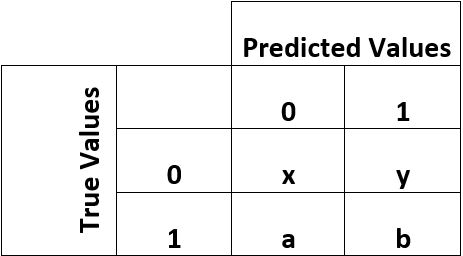
\includegraphics{confusion_matrix.jpg}
\caption{title}
\end{figure}

    \begin{Verbatim}[commandchars=\\\{\}]
{\color{incolor}In [{\color{incolor}46}]:} \PY{c+c1}{\PYZsh{} Printing Confusion Matrix and related metrics for evaluating the model}
         \PY{n}{cm1DT} \PY{o}{=} \PY{n}{sklearn}\PY{o}{.}\PY{n}{metrics}\PY{o}{.}\PY{n}{confusion\PYZus{}matrix}\PY{p}{(}\PY{n}{y\PYZus{}pred}\PY{o}{=}\PY{n}{y\PYZus{}pred}\PY{p}{,}\PY{n}{y\PYZus{}true}\PY{o}{=}\PY{n}{y\PYZus{}test}\PY{p}{)}
         \PY{n}{Classification\PYZus{}Analysis}\PY{p}{(}\PY{n}{cm1DT}\PY{p}{)}
\end{Verbatim}


    \begin{Verbatim}[commandchars=\\\{\}]
Confusion Matrix : 
 [[6800 3552]
 [3889 6759]]
Accuracy :  0.6456666666666667
Specificity :  0.6361680232014221
Sensitivity :  0.6347670924117205
Precision :  0.6555135292406168



    \end{Verbatim}

    We can also study the ROC curve for the model1:

    \begin{Verbatim}[commandchars=\\\{\}]
{\color{incolor}In [{\color{incolor}47}]:} \PY{c+c1}{\PYZsh{} Defining ROC\PYZhy{}plotting function:}
         
         \PY{k}{def} \PY{n+nf}{plot\PYZus{}roc}\PY{p}{(}\PY{n}{fpr}\PY{p}{,}\PY{n}{tpr}\PY{p}{,}\PY{n}{roc\PYZus{}auc}\PY{p}{,} \PY{n}{color\PYZus{}curve}\PY{p}{)}\PY{p}{:}
             \PY{n}{plt}\PY{o}{.}\PY{n}{title}\PY{p}{(}\PY{l+s+s1}{\PYZsq{}}\PY{l+s+s1}{Receiver Operating Characteristic}\PY{l+s+s1}{\PYZsq{}}\PY{p}{)}
             \PY{n}{plt}\PY{o}{.}\PY{n}{plot}\PY{p}{(}\PY{n}{fpr}\PY{p}{,} \PY{n}{tpr}\PY{p}{,} \PY{n}{color}\PY{o}{=}\PY{n}{color\PYZus{}curve}\PY{p}{,} \PY{n}{label} \PY{o}{=} \PY{l+s+s1}{\PYZsq{}}\PY{l+s+s1}{AUC = }\PY{l+s+si}{\PYZpc{}0.2f}\PY{l+s+s1}{\PYZsq{}} \PY{o}{\PYZpc{}} \PY{n}{roc\PYZus{}auc}\PY{p}{)}
             \PY{n}{plt}\PY{o}{.}\PY{n}{legend}\PY{p}{(}\PY{n}{loc} \PY{o}{=} \PY{l+s+s1}{\PYZsq{}}\PY{l+s+s1}{lower right}\PY{l+s+s1}{\PYZsq{}}\PY{p}{)}
             \PY{n}{plt}\PY{o}{.}\PY{n}{plot}\PY{p}{(}\PY{p}{[}\PY{l+m+mi}{0}\PY{p}{,} \PY{l+m+mi}{1}\PY{p}{]}\PY{p}{,} \PY{p}{[}\PY{l+m+mi}{0}\PY{p}{,} \PY{l+m+mi}{1}\PY{p}{]}\PY{p}{,}\PY{l+s+s1}{\PYZsq{}}\PY{l+s+s1}{r\PYZhy{}\PYZhy{}}\PY{l+s+s1}{\PYZsq{}}\PY{p}{,} \PY{n}{label} \PY{o}{=} \PY{l+s+s1}{\PYZsq{}}\PY{l+s+s1}{Baseline}\PY{l+s+s1}{\PYZsq{}}\PY{p}{)}
             \PY{n}{plt}\PY{o}{.}\PY{n}{xlim}\PY{p}{(}\PY{p}{[}\PY{l+m+mi}{0}\PY{p}{,} \PY{l+m+mi}{1}\PY{p}{]}\PY{p}{)}
             \PY{n}{plt}\PY{o}{.}\PY{n}{ylim}\PY{p}{(}\PY{p}{[}\PY{l+m+mi}{0}\PY{p}{,} \PY{l+m+mi}{1}\PY{p}{]}\PY{p}{)}
             \PY{n}{plt}\PY{o}{.}\PY{n}{ylabel}\PY{p}{(}\PY{l+s+s1}{\PYZsq{}}\PY{l+s+s1}{True Positive Rate}\PY{l+s+s1}{\PYZsq{}}\PY{p}{)}
             \PY{n}{plt}\PY{o}{.}\PY{n}{xlabel}\PY{p}{(}\PY{l+s+s1}{\PYZsq{}}\PY{l+s+s1}{False Positive Rate}\PY{l+s+s1}{\PYZsq{}}\PY{p}{)}
             \PY{n}{plt}\PY{o}{.}\PY{n}{show}\PY{p}{(}\PY{p}{)}
             \PY{k}{return}\PY{p}{;}
\end{Verbatim}


    \begin{Verbatim}[commandchars=\\\{\}]
{\color{incolor}In [{\color{incolor}48}]:} \PY{c+c1}{\PYZsh{} calculate the fpr and tpr for all thresholds of  decision tree}
         \PY{n}{prob\PYZus{}dt} \PY{o}{=} \PY{n}{model1}\PY{o}{.}\PY{n}{predict\PYZus{}proba}\PY{p}{(}\PY{n}{x\PYZus{}test}\PY{p}{)}
         \PY{n}{pred\PYZus{}dt} \PY{o}{=} \PY{n}{prob\PYZus{}dt}\PY{p}{[}\PY{p}{:}\PY{p}{,}\PY{l+m+mi}{1}\PY{p}{]}
         \PY{n}{fpr}\PY{p}{,} \PY{n}{tpr}\PY{p}{,} \PY{n}{threshold} \PY{o}{=} \PY{n}{sklearn}\PY{o}{.}\PY{n}{metrics}\PY{o}{.}\PY{n}{roc\PYZus{}curve}\PY{p}{(}\PY{n}{y\PYZus{}test}\PY{p}{,} \PY{n}{pred\PYZus{}dt}\PY{p}{)}
         \PY{n}{roc\PYZus{}auc} \PY{o}{=} \PY{n}{sklearn}\PY{o}{.}\PY{n}{metrics}\PY{o}{.}\PY{n}{auc}\PY{p}{(}\PY{n}{fpr}\PY{p}{,} \PY{n}{tpr}\PY{p}{)}
\end{Verbatim}


    \begin{Verbatim}[commandchars=\\\{\}]
{\color{incolor}In [{\color{incolor}49}]:} \PY{c+c1}{\PYZsh{} plotting the roc curve for decision tree}
         \PY{n}{plot\PYZus{}roc}\PY{p}{(}\PY{n}{fpr}\PY{p}{,}\PY{n}{tpr}\PY{p}{,}\PY{n}{roc\PYZus{}auc}\PY{p}{,}\PY{l+s+s1}{\PYZsq{}}\PY{l+s+s1}{\PYZsh{}495aa1}\PY{l+s+s1}{\PYZsq{}}\PY{p}{)}
         
         \PY{c+c1}{\PYZsh{}\PYZsh{} Solution Ends here}
\end{Verbatim}


    \begin{center}
    \adjustimage{max size={0.9\linewidth}{0.9\paperheight}}{output_67_0.png}
    \end{center}
    { \hspace*{\fill} \\}
    
    \paragraph{7.2}\label{section}

Set up the depth of the tree using cross-validation on the dataset
\texttt{(X\_train,\ y\_train)} in order to increase quality of the
model. Use \texttt{GridSearchCV} with 5 folds. Fix
\texttt{random\_state=20} and change \texttt{max\_depth} from 4 to 8.

\begin{itemize}
\item
  Draw the plot to show how mean accuracy is changing in regards to
  \texttt{max\_depth} value on cross-validation.
\item
  Print the best value of \texttt{max\_depth}. Also compute accuracy on
  holdout data.
\end{itemize}

    \begin{Verbatim}[commandchars=\\\{\}]
{\color{incolor}In [{\color{incolor}50}]:} \PY{c+c1}{\PYZsh{}\PYZsh{}\PYZsh{} Solution for problem\PYZhy{}7.2 Starts Here}
         
         \PY{n}{accuracy}\PY{o}{=}\PY{p}{[}\PY{p}{]}
         \PY{n}{maxDepth}\PY{o}{=}\PY{p}{[}\PY{p}{]}
         \PY{k}{for} \PY{n}{x} \PY{o+ow}{in} \PY{n+nb}{range}\PY{p}{(}\PY{l+m+mi}{4}\PY{p}{,}\PY{l+m+mi}{9}\PY{p}{)}\PY{p}{:}
             \PY{n}{model\PYZus{}t}\PY{o}{=} \PY{n}{sklearn}\PY{o}{.}\PY{n}{tree}\PY{o}{.}\PY{n}{DecisionTreeClassifier}\PY{p}{(}\PY{n}{max\PYZus{}depth}\PY{o}{=}\PY{n}{x}\PY{p}{)}
             \PY{n}{model\PYZus{}tf}\PY{o}{=} \PY{n}{model\PYZus{}t}\PY{o}{.}\PY{n}{fit}\PY{p}{(}\PY{n}{x\PYZus{}train}\PY{p}{,}\PY{n}{y\PYZus{}train}\PY{p}{)}
             \PY{n}{y\PYZus{}pred}\PY{o}{=} \PY{n}{model\PYZus{}tf}\PY{o}{.}\PY{n}{predict}\PY{p}{(}\PY{n}{x\PYZus{}test}\PY{p}{)}
             \PY{n}{cm}\PY{o}{=} \PY{n}{sklearn}\PY{o}{.}\PY{n}{metrics}\PY{o}{.}\PY{n}{confusion\PYZus{}matrix}\PY{p}{(}\PY{n}{y\PYZus{}pred}\PY{o}{=}\PY{n}{y\PYZus{}pred}\PY{p}{,}\PY{n}{y\PYZus{}true}\PY{o}{=}\PY{n}{y\PYZus{}test}\PY{p}{)}
             \PY{n}{total}\PY{o}{=}\PY{n+nb}{sum}\PY{p}{(}\PY{n+nb}{sum}\PY{p}{(}\PY{n}{cm}\PY{p}{)}\PY{p}{)}
             \PY{n}{acc}\PY{o}{=}\PY{p}{(}\PY{n}{cm}\PY{p}{[}\PY{l+m+mi}{0}\PY{p}{,}\PY{l+m+mi}{0}\PY{p}{]}\PY{o}{+}\PY{n}{cm}\PY{p}{[}\PY{l+m+mi}{1}\PY{p}{,}\PY{l+m+mi}{1}\PY{p}{]}\PY{p}{)}\PY{o}{/}\PY{n}{total}
             \PY{n}{accuracy}\PY{o}{.}\PY{n}{append}\PY{p}{(}\PY{n}{acc}\PY{p}{)}
             \PY{n}{maxDepth}\PY{o}{.}\PY{n}{append}\PY{p}{(}\PY{n}{x}\PY{p}{)}
             
\end{Verbatim}


    \begin{Verbatim}[commandchars=\\\{\}]
{\color{incolor}In [{\color{incolor}51}]:} \PY{n}{plt}\PY{o}{.}\PY{n}{plot}\PY{p}{(}\PY{n}{maxDepth}\PY{p}{,} \PY{n}{accuracy}\PY{p}{,} \PY{l+s+s1}{\PYZsq{}}\PY{l+s+s1}{\PYZhy{}g}\PY{l+s+s1}{\PYZsq{}}\PY{p}{)}
         \PY{n}{plt}\PY{o}{.}\PY{n}{title}\PY{p}{(}\PY{l+s+s1}{\PYZsq{}}\PY{l+s+s1}{Accuracy vs Max\PYZhy{}Depth}\PY{l+s+s1}{\PYZsq{}}\PY{p}{)}
         \PY{n}{plt}\PY{o}{.}\PY{n}{xlim}\PY{p}{(}\PY{p}{[}\PY{l+m+mi}{4}\PY{p}{,}\PY{l+m+mi}{9}\PY{p}{]}\PY{p}{)}
         \PY{n}{plt}\PY{o}{.}\PY{n}{xlabel}\PY{p}{(}\PY{l+s+s1}{\PYZsq{}}\PY{l+s+s1}{Max Depth}\PY{l+s+s1}{\PYZsq{}}\PY{p}{)}
         \PY{n}{plt}\PY{o}{.}\PY{n}{ylabel}\PY{p}{(}\PY{l+s+s1}{\PYZsq{}}\PY{l+s+s1}{Accuracy}\PY{l+s+s1}{\PYZsq{}}\PY{p}{)}
\end{Verbatim}


\begin{Verbatim}[commandchars=\\\{\}]
{\color{outcolor}Out[{\color{outcolor}51}]:} Text(0,0.5,'Accuracy')
\end{Verbatim}
            
    \begin{center}
    \adjustimage{max size={0.9\linewidth}{0.9\paperheight}}{output_70_1.png}
    \end{center}
    { \hspace*{\fill} \\}
    
    \begin{Verbatim}[commandchars=\\\{\}]
{\color{incolor}In [{\color{incolor}52}]:} \PY{n}{parameters}\PY{o}{=}\PY{p}{\PYZob{}}\PY{l+s+s1}{\PYZsq{}}\PY{l+s+s1}{max\PYZus{}depth}\PY{l+s+s1}{\PYZsq{}}\PY{p}{:} \PY{n+nb}{range}\PY{p}{(}\PY{l+m+mi}{4}\PY{p}{,}\PY{l+m+mi}{9}\PY{p}{)}\PY{p}{\PYZcb{}}
         \PY{n}{clf}\PY{o}{=}\PY{n}{sklearn}\PY{o}{.}\PY{n}{model\PYZus{}selection}\PY{o}{.}\PY{n}{GridSearchCV}\PY{p}{(}\PY{n}{decision\PYZus{}tree}\PY{p}{,}\PY{n}{parameters}\PY{p}{,}\PY{n}{cv}\PY{o}{=}\PY{l+m+mi}{5}\PY{p}{)}
         \PY{n}{DT\PYZus{}CV}\PY{o}{=}\PY{n}{clf}\PY{o}{.}\PY{n}{fit}\PY{p}{(}\PY{n}{x\PYZus{}train}\PY{p}{,}\PY{n}{y\PYZus{}train}\PY{p}{)}
         
         \PY{n}{DT\PYZus{}CV}\PY{o}{.}\PY{n}{best\PYZus{}estimator\PYZus{}}
         
         \PY{c+c1}{\PYZsh{}\PYZsh{} Solution Ends here}
\end{Verbatim}


\begin{Verbatim}[commandchars=\\\{\}]
{\color{outcolor}Out[{\color{outcolor}52}]:} DecisionTreeClassifier(class\_weight=None, criterion='gini', max\_depth=6,
                     max\_features=None, max\_leaf\_nodes=None,
                     min\_impurity\_decrease=0.0, min\_impurity\_split=None,
                     min\_samples\_leaf=1, min\_samples\_split=2,
                     min\_weight\_fraction\_leaf=0.0, presort=False, random\_state=20,
                     splitter='best')
\end{Verbatim}
            
    \paragraph{7.3}\label{section}

What conclusions can you derive from model how does these conclusions
fit to your understanding cardiovascular disease

    \begin{Verbatim}[commandchars=\\\{\}]
{\color{incolor}In [{\color{incolor}53}]:} \PY{c+c1}{\PYZsh{}\PYZsh{}\PYZsh{} Solution for problem\PYZhy{}7.3 Starts Here}
         
         \PY{c+c1}{\PYZsh{} Before drawing conclusions we can study the decision tree with best estimator:}
         \PY{n}{model2}\PY{o}{=} \PY{n}{sklearn}\PY{o}{.}\PY{n}{tree}\PY{o}{.}\PY{n}{DecisionTreeClassifier}\PY{p}{(}\PY{n}{class\PYZus{}weight}\PY{o}{=}\PY{k+kc}{None}\PY{p}{,} \PY{n}{criterion}\PY{o}{=}\PY{l+s+s1}{\PYZsq{}}\PY{l+s+s1}{gini}\PY{l+s+s1}{\PYZsq{}}\PY{p}{,} \PY{n}{max\PYZus{}depth}\PY{o}{=}\PY{l+m+mi}{6}\PY{p}{,}
                     \PY{n}{max\PYZus{}features}\PY{o}{=}\PY{k+kc}{None}\PY{p}{,} \PY{n}{max\PYZus{}leaf\PYZus{}nodes}\PY{o}{=}\PY{k+kc}{None}\PY{p}{,}
                     \PY{n}{min\PYZus{}impurity\PYZus{}decrease}\PY{o}{=}\PY{l+m+mf}{0.0}\PY{p}{,} \PY{n}{min\PYZus{}impurity\PYZus{}split}\PY{o}{=}\PY{k+kc}{None}\PY{p}{,}
                     \PY{n}{min\PYZus{}samples\PYZus{}leaf}\PY{o}{=}\PY{l+m+mi}{1}\PY{p}{,} \PY{n}{min\PYZus{}samples\PYZus{}split}\PY{o}{=}\PY{l+m+mi}{2}\PY{p}{,}
                     \PY{n}{min\PYZus{}weight\PYZus{}fraction\PYZus{}leaf}\PY{o}{=}\PY{l+m+mf}{0.0}\PY{p}{,} \PY{n}{presort}\PY{o}{=}\PY{k+kc}{False}\PY{p}{,} \PY{n}{random\PYZus{}state}\PY{o}{=}\PY{l+m+mi}{20}\PY{p}{,}
                     \PY{n}{splitter}\PY{o}{=}\PY{l+s+s1}{\PYZsq{}}\PY{l+s+s1}{best}\PY{l+s+s1}{\PYZsq{}}\PY{p}{)}
         
         \PY{n}{DT\PYZus{}best}\PY{o}{=} \PY{n}{model2}\PY{o}{.}\PY{n}{fit}\PY{p}{(}\PY{n}{x\PYZus{}train}\PY{p}{,} \PY{n}{y\PYZus{}train}\PY{p}{)}
\end{Verbatim}


    \begin{Verbatim}[commandchars=\\\{\}]
{\color{incolor}In [{\color{incolor}54}]:} \PY{c+c1}{\PYZsh{} Making predictions with model2:}
         \PY{n}{y\PYZus{}pred2}\PY{o}{=} \PY{n}{DT\PYZus{}best}\PY{o}{.}\PY{n}{predict}\PY{p}{(}\PY{n}{x\PYZus{}test}\PY{p}{)}
\end{Verbatim}


    \begin{Verbatim}[commandchars=\\\{\}]
{\color{incolor}In [{\color{incolor}55}]:} \PY{c+c1}{\PYZsh{} Rendering Decision tree with best estimator:}
         \PY{n}{dot\PYZus{}data} \PY{o}{=} \PY{n}{StringIO}\PY{p}{(}\PY{p}{)}
         \PY{n}{export\PYZus{}graphviz}\PY{p}{(}\PY{n}{model2}\PY{p}{,} \PY{n}{out\PYZus{}file}\PY{o}{=}\PY{n}{dot\PYZus{}data}\PY{p}{,}  
                         \PY{n}{filled}\PY{o}{=}\PY{k+kc}{True}\PY{p}{,} \PY{n}{rounded}\PY{o}{=}\PY{k+kc}{True}\PY{p}{,}
                         \PY{n}{special\PYZus{}characters}\PY{o}{=}\PY{k+kc}{True}\PY{p}{,}\PY{n}{feature\PYZus{}names}\PY{o}{=}\PY{n+nb}{list}\PY{p}{(}\PY{n}{x\PYZus{}train}\PY{o}{.}\PY{n}{columns}\PY{p}{)}\PY{p}{)}
         \PY{n}{graph1} \PY{o}{=} \PY{n}{pydotplus}\PY{o}{.}\PY{n}{graph\PYZus{}from\PYZus{}dot\PYZus{}data}\PY{p}{(}\PY{n}{dot\PYZus{}data}\PY{o}{.}\PY{n}{getvalue}\PY{p}{(}\PY{p}{)}\PY{p}{)}  
         \PY{n}{Image}\PY{p}{(}\PY{n}{graph1}\PY{o}{.}\PY{n}{create\PYZus{}png}\PY{p}{(}\PY{p}{)}\PY{p}{)}
\end{Verbatim}

\texttt{\color{outcolor}Out[{\color{outcolor}55}]:}
    
    \begin{center}
    \adjustimage{max size={0.9\linewidth}{0.9\paperheight}}{output_75_0.png}
    \end{center}
    { \hspace*{\fill} \\}
    

    \begin{Verbatim}[commandchars=\\\{\}]
{\color{incolor}In [{\color{incolor}56}]:} \PY{c+c1}{\PYZsh{} Printing Confusion Matrix and related metrics for evaluating the model}
         \PY{n}{cm2DT} \PY{o}{=} \PY{n}{sklearn}\PY{o}{.}\PY{n}{metrics}\PY{o}{.}\PY{n}{confusion\PYZus{}matrix}\PY{p}{(}\PY{n}{y\PYZus{}pred}\PY{o}{=}\PY{n}{y\PYZus{}pred2}\PY{p}{,}\PY{n}{y\PYZus{}true}\PY{o}{=}\PY{n}{y\PYZus{}test}\PY{p}{)}
         \PY{n}{Classification\PYZus{}Analysis}\PY{p}{(}\PY{n}{cm2DT}\PY{p}{)}
\end{Verbatim}


    \begin{Verbatim}[commandchars=\\\{\}]
Confusion Matrix : 
 [[5910 4442]
 [2832 7816]]
Accuracy :  0.6536190476190477
Specificity :  0.6760466712422787
Sensitivity :  0.7340345604808415
Precision :  0.6376244085495186



    \end{Verbatim}

    \begin{Verbatim}[commandchars=\\\{\}]
{\color{incolor}In [{\color{incolor}57}]:} \PY{c+c1}{\PYZsh{} calculate the fpr and tpr for all thresholds of Random Forest}
         \PY{n}{prob\PYZus{}dt2} \PY{o}{=} \PY{n}{model2}\PY{o}{.}\PY{n}{predict\PYZus{}proba}\PY{p}{(}\PY{n}{x\PYZus{}test}\PY{p}{)}
         \PY{n}{pred\PYZus{}dt2} \PY{o}{=} \PY{n}{prob\PYZus{}dt2}\PY{p}{[}\PY{p}{:}\PY{p}{,}\PY{l+m+mi}{1}\PY{p}{]}
         \PY{n}{fpr2}\PY{p}{,} \PY{n}{tpr2}\PY{p}{,} \PY{n}{threshold2} \PY{o}{=} \PY{n}{sklearn}\PY{o}{.}\PY{n}{metrics}\PY{o}{.}\PY{n}{roc\PYZus{}curve}\PY{p}{(}\PY{n}{y\PYZus{}test}\PY{p}{,} \PY{n}{pred\PYZus{}dt2}\PY{p}{)}
         \PY{n}{roc\PYZus{}auc2} \PY{o}{=} \PY{n}{sklearn}\PY{o}{.}\PY{n}{metrics}\PY{o}{.}\PY{n}{auc}\PY{p}{(}\PY{n}{fpr2}\PY{p}{,} \PY{n}{tpr2}\PY{p}{)}
         
         \PY{c+c1}{\PYZsh{} plotting the roc curve for decision tree}
         \PY{n}{plot\PYZus{}roc}\PY{p}{(}\PY{n}{fpr2}\PY{p}{,}\PY{n}{tpr2}\PY{p}{,}\PY{n}{roc\PYZus{}auc2}\PY{p}{,}\PY{l+s+s1}{\PYZsq{}}\PY{l+s+s1}{\PYZsh{}495aa1}\PY{l+s+s1}{\PYZsq{}}\PY{p}{)}
\end{Verbatim}


    \begin{center}
    \adjustimage{max size={0.9\linewidth}{0.9\paperheight}}{output_77_0.png}
    \end{center}
    { \hspace*{\fill} \\}
    
    \subsubsection{\texorpdfstring{\emph{Conclusion:}}{Conclusion:}}\label{conclusion}

\emph{After analyzing two different decision trees we can infer that, in
general the factors that are mainly responsible for cardio vascular
diseases are Blood Pressure, Age and Cholestrol. People with blood
pressure more than 140 or less than 90 are more likely to be prone
towards Cardio Vascular Disease. This probability further increase if
the person is older than 55. These conclusions fits very precise to what
cases are recorded about cardio vascular disease.}

    \begin{Verbatim}[commandchars=\\\{\}]
{\color{incolor}In [{\color{incolor}58}]:} \PY{c+c1}{\PYZsh{}\PYZsh{}\PYZsh{} Solution Ends here.}
\end{Verbatim}


    \subsubsection{Problem 8:}\label{problem-8}

A unit of equipment operates at a temperature that is known to be
closely linked to the ambient temperature.

    \begin{Verbatim}[commandchars=\\\{\}]
{\color{incolor}In [{\color{incolor}59}]:} \PY{n}{resp} \PY{o}{=} \PY{n}{urlopen}\PY{p}{(}\PY{l+s+s2}{\PYZdq{}}\PY{l+s+s2}{https://s3.amazonaws.com/aq\PYZhy{}web\PYZhy{}library/daily\PYZus{}temp.csv.zip}\PY{l+s+s2}{\PYZdq{}}\PY{p}{)}
         \PY{n}{zipfile\PYZus{}} \PY{o}{=} \PY{n}{ZipFile}\PY{p}{(}\PY{n}{BytesIO}\PY{p}{(}\PY{n}{resp}\PY{o}{.}\PY{n}{read}\PY{p}{(}\PY{p}{)}\PY{p}{)}\PY{p}{)}
         \PY{n}{daily\PYZus{}temp} \PY{o}{=} \PY{n}{pd}\PY{o}{.}\PY{n}{read\PYZus{}csv}\PY{p}{(}\PY{n}{zipfile\PYZus{}}\PY{o}{.}\PY{n}{open}\PY{p}{(}\PY{l+s+s1}{\PYZsq{}}\PY{l+s+s1}{daily\PYZus{}temp.csv}\PY{l+s+s1}{\PYZsq{}}\PY{p}{)}\PY{p}{)}
\end{Verbatim}


    \paragraph{8.1 using the following dataframe, construct a time series
visual of the equipment
temperature}\label{using-the-following-dataframe-construct-a-time-series-visual-of-the-equipment-temperature}

    \begin{Verbatim}[commandchars=\\\{\}]
{\color{incolor}In [{\color{incolor}60}]:} \PY{c+c1}{\PYZsh{}\PYZsh{}\PYZsh{} Solution for problem\PYZhy{}8.1 Starts Here}
         
         \PY{c+c1}{\PYZsh{} To get better visualizations we can resample the data monthly.}
         \PY{n}{daily\PYZus{}temp}\PY{o}{.}\PY{n}{Date} \PY{o}{=} \PY{n}{pd}\PY{o}{.}\PY{n}{to\PYZus{}datetime}\PY{p}{(}\PY{n}{daily\PYZus{}temp}\PY{o}{.}\PY{n}{Date}\PY{p}{)}
         \PY{n}{df\PYZus{}resampled} \PY{o}{=} \PY{n}{daily\PYZus{}temp}\PY{o}{.}\PY{n}{resample}\PY{p}{(}\PY{l+s+s1}{\PYZsq{}}\PY{l+s+s1}{M}\PY{l+s+s1}{\PYZsq{}}\PY{p}{,} \PY{n}{on}\PY{o}{=}\PY{l+s+s1}{\PYZsq{}}\PY{l+s+s1}{Date}\PY{l+s+s1}{\PYZsq{}}\PY{p}{)}\PY{o}{.}\PY{n}{sum}\PY{p}{(}\PY{p}{)}
         \PY{n}{df\PYZus{}resampled}\PY{p}{[}\PY{l+s+s1}{\PYZsq{}}\PY{l+s+s1}{Equipment Temperature (F)}\PY{l+s+s1}{\PYZsq{}}\PY{p}{]}\PY{o}{.}\PY{n}{plot}\PY{p}{(}\PY{n}{figsize}\PY{o}{=}\PY{p}{(}\PY{l+m+mi}{15}\PY{p}{,} \PY{l+m+mi}{6}\PY{p}{)}\PY{p}{)}
         \PY{n}{plt}\PY{o}{.}\PY{n}{show}\PY{p}{(}\PY{p}{)}
\end{Verbatim}


    \begin{center}
    \adjustimage{max size={0.9\linewidth}{0.9\paperheight}}{output_83_0.png}
    \end{center}
    { \hspace*{\fill} \\}
    
    \begin{Verbatim}[commandchars=\\\{\}]
{\color{incolor}In [{\color{incolor}61}]:} \PY{c+c1}{\PYZsh{} Before starting visualization we will set date as index for the dataframe:}
         \PY{n}{daily\PYZus{}temp}\PY{o}{.}\PY{n}{set\PYZus{}index}\PY{p}{(}\PY{l+s+s1}{\PYZsq{}}\PY{l+s+s1}{Date}\PY{l+s+s1}{\PYZsq{}}\PY{p}{,} \PY{n}{inplace}\PY{o}{=}\PY{k+kc}{True}\PY{p}{)}
         
         \PY{c+c1}{\PYZsh{} Now we will check for null values in the Timeseries:}
         \PY{n}{daily\PYZus{}temp}\PY{o}{.}\PY{n}{isnull}\PY{p}{(}\PY{p}{)}\PY{o}{.}\PY{n}{sum}\PY{p}{(}\PY{p}{)}
\end{Verbatim}


\begin{Verbatim}[commandchars=\\\{\}]
{\color{outcolor}Out[{\color{outcolor}61}]:} Ambient Temperature (F)      5169
         Equipment Temperature (F)    5169
         dtype: int64
\end{Verbatim}
            
    \textbf{Since we have Null values we have two options:} 1. We can remove
the null entries and plot the available data 2. We can fill the null
values. For now let's fill values by rolling mean.

To retain the data, create different frameworks instead of editing the
same.

    \begin{Verbatim}[commandchars=\\\{\}]
{\color{incolor}In [{\color{incolor}62}]:} \PY{c+c1}{\PYZsh{} 1. Remove the null entries and plot the Equipment Temperature and creating a new data frame:}
         \PY{n}{df\PYZus{}no\PYZus{}null}\PY{o}{=}\PY{n}{daily\PYZus{}temp}\PY{p}{[} \PY{l+s+s1}{\PYZsq{}}\PY{l+s+s1}{Equipment Temperature (F)}\PY{l+s+s1}{\PYZsq{}}\PY{p}{]}\PY{o}{.}\PY{n}{dropna}\PY{p}{(}\PY{p}{)}
\end{Verbatim}


    \begin{Verbatim}[commandchars=\\\{\}]
{\color{incolor}In [{\color{incolor}63}]:} \PY{c+c1}{\PYZsh{} Visualize Equipment Temperature against date:}
         \PY{n}{df\PYZus{}no\PYZus{}null}\PY{o}{.}\PY{n}{plot}\PY{p}{(}\PY{n}{figsize}\PY{o}{=}\PY{p}{(}\PY{l+m+mi}{15}\PY{p}{,} \PY{l+m+mi}{6}\PY{p}{)}\PY{p}{)}
         \PY{n}{plt}\PY{o}{.}\PY{n}{show}\PY{p}{(}\PY{p}{)}
\end{Verbatim}


    \begin{center}
    \adjustimage{max size={0.9\linewidth}{0.9\paperheight}}{output_87_0.png}
    \end{center}
    { \hspace*{\fill} \\}
    
    \begin{Verbatim}[commandchars=\\\{\}]
{\color{incolor}In [{\color{incolor}64}]:} \PY{c+c1}{\PYZsh{} 2. Fill null values with rolling mean and create a new data frame:}
         \PY{n}{df\PYZus{}roll\PYZus{}mean} \PY{o}{=} \PY{n}{daily\PYZus{}temp}\PY{p}{[}\PY{l+s+s1}{\PYZsq{}}\PY{l+s+s1}{Equipment Temperature (F)}\PY{l+s+s1}{\PYZsq{}}\PY{p}{]}\PY{o}{.}\PY{n}{rolling}\PY{p}{(}\PY{l+m+mi}{12}\PY{p}{,}\PY{n}{center}\PY{o}{=}\PY{k+kc}{True}\PY{p}{,}\PY{n}{min\PYZus{}periods}\PY{o}{=}\PY{l+m+mi}{1}\PY{p}{)}\PY{o}{.}\PY{n}{mean}\PY{p}{(}\PY{p}{)}
\end{Verbatim}


    \begin{Verbatim}[commandchars=\\\{\}]
{\color{incolor}In [{\color{incolor}65}]:} \PY{c+c1}{\PYZsh{} Visualize Equipment Temperature against date:}
         \PY{n}{df\PYZus{}roll\PYZus{}mean}\PY{o}{.}\PY{n}{plot}\PY{p}{(}\PY{n}{figsize}\PY{o}{=}\PY{p}{(}\PY{l+m+mi}{15}\PY{p}{,} \PY{l+m+mi}{6}\PY{p}{)}\PY{p}{)}
         \PY{n}{plt}\PY{o}{.}\PY{n}{show}\PY{p}{(}\PY{p}{)}
\end{Verbatim}


    \begin{center}
    \adjustimage{max size={0.9\linewidth}{0.9\paperheight}}{output_89_0.png}
    \end{center}
    { \hspace*{\fill} \\}
    
    \paragraph{8.2 Some of the equipmentd data is missing. Based on the
available data, fill in the gaps in a sensible
way.}\label{some-of-the-equipmentd-data-is-missing.-based-on-the-available-data-fill-in-the-gaps-in-a-sensible-way.}

    \begin{Verbatim}[commandchars=\\\{\}]
{\color{incolor}In [{\color{incolor}66}]:} \PY{c+c1}{\PYZsh{}\PYZsh{}\PYZsh{} Solution for problem\PYZhy{}8.2 Starts Here}
         
         \PY{c+c1}{\PYZsh{} We have already filled null values with rolling mean and is stored in \PYZsq{}df\PYZus{}roll\PYZus{}mean\PYZsq{}. Now we will use different interpolate methods to fill the value:}
         \PY{n}{InterpolateTime} \PY{o}{=} \PY{n}{daily\PYZus{}temp}\PY{p}{[}\PY{l+s+s1}{\PYZsq{}}\PY{l+s+s1}{Equipment Temperature (F)}\PY{l+s+s1}{\PYZsq{}}\PY{p}{]}\PY{o}{.}\PY{n}{interpolate}\PY{p}{(}\PY{n}{method}\PY{o}{=}\PY{l+s+s1}{\PYZsq{}}\PY{l+s+s1}{time}\PY{l+s+s1}{\PYZsq{}}\PY{p}{)}
         \PY{n}{InterpolatePad} \PY{o}{=} \PY{n}{daily\PYZus{}temp}\PY{p}{[}\PY{l+s+s1}{\PYZsq{}}\PY{l+s+s1}{Equipment Temperature (F)}\PY{l+s+s1}{\PYZsq{}}\PY{p}{]}\PY{o}{.}\PY{n}{interpolate}\PY{p}{(}\PY{n}{method}\PY{o}{=}\PY{l+s+s1}{\PYZsq{}}\PY{l+s+s1}{pad}\PY{l+s+s1}{\PYZsq{}}\PY{p}{)}
         \PY{n}{InterpolateTime\PYZus{}resampled} \PY{o}{=} \PY{n}{df\PYZus{}resampled}\PY{p}{[}\PY{l+s+s1}{\PYZsq{}}\PY{l+s+s1}{Equipment Temperature (F)}\PY{l+s+s1}{\PYZsq{}}\PY{p}{]}\PY{o}{.}\PY{n}{interpolate}\PY{p}{(}\PY{n}{method}\PY{o}{=}\PY{l+s+s1}{\PYZsq{}}\PY{l+s+s1}{time}\PY{l+s+s1}{\PYZsq{}}\PY{p}{)}
         \PY{n}{InterpolatePad\PYZus{}resampled} \PY{o}{=} \PY{n}{df\PYZus{}resampled}\PY{p}{[}\PY{l+s+s1}{\PYZsq{}}\PY{l+s+s1}{Equipment Temperature (F)}\PY{l+s+s1}{\PYZsq{}}\PY{p}{]}\PY{o}{.}\PY{n}{interpolate}\PY{p}{(}\PY{n}{method}\PY{o}{=}\PY{l+s+s1}{\PYZsq{}}\PY{l+s+s1}{pad}\PY{l+s+s1}{\PYZsq{}}\PY{p}{)}
\end{Verbatim}


    \begin{Verbatim}[commandchars=\\\{\}]
{\color{incolor}In [{\color{incolor}67}]:} \PY{n}{InterpolateTime\PYZus{}resampled}\PY{o}{.}\PY{n}{plot}\PY{p}{(}\PY{n}{figsize}\PY{o}{=}\PY{p}{(}\PY{l+m+mi}{15}\PY{p}{,} \PY{l+m+mi}{6}\PY{p}{)}\PY{p}{)}
         \PY{n}{plt}\PY{o}{.}\PY{n}{show}\PY{p}{(}\PY{p}{)}
\end{Verbatim}


    \begin{center}
    \adjustimage{max size={0.9\linewidth}{0.9\paperheight}}{output_92_0.png}
    \end{center}
    { \hspace*{\fill} \\}
    
    \begin{Verbatim}[commandchars=\\\{\}]
{\color{incolor}In [{\color{incolor}68}]:} \PY{n}{InterpolatePad\PYZus{}resampled}\PY{o}{.}\PY{n}{plot}\PY{p}{(}\PY{n}{figsize}\PY{o}{=}\PY{p}{(}\PY{l+m+mi}{15}\PY{p}{,} \PY{l+m+mi}{6}\PY{p}{)}\PY{p}{)}
         \PY{n}{plt}\PY{o}{.}\PY{n}{show}\PY{p}{(}\PY{p}{)}
\end{Verbatim}


    \begin{center}
    \adjustimage{max size={0.9\linewidth}{0.9\paperheight}}{output_93_0.png}
    \end{center}
    { \hspace*{\fill} \\}
    
    \begin{Verbatim}[commandchars=\\\{\}]
{\color{incolor}In [{\color{incolor}69}]:} \PY{n}{InterpolateTime}\PY{o}{.}\PY{n}{plot}\PY{p}{(}\PY{n}{figsize}\PY{o}{=}\PY{p}{(}\PY{l+m+mi}{15}\PY{p}{,} \PY{l+m+mi}{6}\PY{p}{)}\PY{p}{)}
         \PY{n}{plt}\PY{o}{.}\PY{n}{show}\PY{p}{(}\PY{p}{)}
\end{Verbatim}


    \begin{center}
    \adjustimage{max size={0.9\linewidth}{0.9\paperheight}}{output_94_0.png}
    \end{center}
    { \hspace*{\fill} \\}
    
    \begin{Verbatim}[commandchars=\\\{\}]
{\color{incolor}In [{\color{incolor}70}]:} \PY{n}{InterpolatePad}\PY{o}{.}\PY{n}{plot}\PY{p}{(}\PY{n}{figsize}\PY{o}{=}\PY{p}{(}\PY{l+m+mi}{15}\PY{p}{,} \PY{l+m+mi}{6}\PY{p}{)}\PY{p}{)}
         \PY{n}{plt}\PY{o}{.}\PY{n}{show}\PY{p}{(}\PY{p}{)}
\end{Verbatim}


    \begin{center}
    \adjustimage{max size={0.9\linewidth}{0.9\paperheight}}{output_95_0.png}
    \end{center}
    { \hspace*{\fill} \\}
    
    \section{Conclusion:}\label{conclusion}

\emph{This timeseries dataset can be visualized in many way and it is
recommended to visualize data set before using it to train a model as a
visualization gives a better intution about the data-flow or pattern
even if there are several missing values in it.} \emph{Here we have
visualized both resampled and raw dataset to explain how resampling
technique can be helpful while taking insights from the data. In both
visualizations, the summer and winter can be observed and a resampled
data visualization gives better picture of this.}

    \subsubsection{Problem 9:}\label{problem-9}

Three files contain 30 days of data collected in January 2019. Merge
into a single dataframe.

    \begin{Verbatim}[commandchars=\\\{\}]
{\color{incolor}In [{\color{incolor}71}]:} \PY{n}{resp} \PY{o}{=} \PY{n}{urlopen}\PY{p}{(}\PY{l+s+s2}{\PYZdq{}}\PY{l+s+s2}{https://s3.amazonaws.com/aq\PYZhy{}web\PYZhy{}library/files.zip}\PY{l+s+s2}{\PYZdq{}}\PY{p}{)}
         \PY{n}{zipfile\PYZus{}} \PY{o}{=} \PY{n}{ZipFile}\PY{p}{(}\PY{n}{BytesIO}\PY{p}{(}\PY{n}{resp}\PY{o}{.}\PY{n}{read}\PY{p}{(}\PY{p}{)}\PY{p}{)}\PY{p}{)}
         \PY{n}{files1} \PY{o}{=} \PY{n}{pd}\PY{o}{.}\PY{n}{read\PYZus{}csv}\PY{p}{(}\PY{n}{zipfile\PYZus{}}\PY{o}{.}\PY{n}{open}\PY{p}{(}\PY{l+s+s1}{\PYZsq{}}\PY{l+s+s1}{file1.csv}\PY{l+s+s1}{\PYZsq{}}\PY{p}{)}\PY{p}{)}
         \PY{n}{files2} \PY{o}{=} \PY{n}{pd}\PY{o}{.}\PY{n}{read\PYZus{}csv}\PY{p}{(}\PY{n}{zipfile\PYZus{}}\PY{o}{.}\PY{n}{open}\PY{p}{(}\PY{l+s+s1}{\PYZsq{}}\PY{l+s+s1}{file2.csv}\PY{l+s+s1}{\PYZsq{}}\PY{p}{)}\PY{p}{)}
         \PY{n}{files3} \PY{o}{=} \PY{n}{pd}\PY{o}{.}\PY{n}{read\PYZus{}csv}\PY{p}{(}\PY{n}{zipfile\PYZus{}}\PY{o}{.}\PY{n}{open}\PY{p}{(}\PY{l+s+s1}{\PYZsq{}}\PY{l+s+s1}{file3.csv}\PY{l+s+s1}{\PYZsq{}}\PY{p}{)}\PY{p}{)}
\end{Verbatim}


    \begin{Verbatim}[commandchars=\\\{\}]
{\color{incolor}In [{\color{incolor}72}]:} \PY{c+c1}{\PYZsh{}\PYZsh{}\PYZsh{} Solution for problem\PYZhy{}9 Starts Here}
         
         \PY{c+c1}{\PYZsh{} Before start merging the dataframes we will create a \PYZsq{}Day\PYZsq{} column in files2:}
         \PY{n}{Day}\PY{o}{=}\PY{p}{[}\PY{p}{]}
         \PY{k}{for} \PY{n}{x} \PY{o+ow}{in} \PY{n}{files2}\PY{o}{.}\PY{n}{time\PYZus{}stamp}\PY{p}{:}
             \PY{n}{Day}\PY{o}{.}\PY{n}{append}\PY{p}{(}\PY{n}{x}\PY{o}{.}\PY{n}{split}\PY{p}{(}\PY{p}{)}\PY{p}{[}\PY{l+m+mi}{0}\PY{p}{]}\PY{o}{.}\PY{n}{replace}\PY{p}{(}\PY{l+s+s1}{\PYZsq{}}\PY{l+s+s1}{2019\PYZhy{}01\PYZhy{}}\PY{l+s+s1}{\PYZsq{}}\PY{p}{,}\PY{l+s+s1}{\PYZsq{}}\PY{l+s+s1}{Jan \PYZhy{}}\PY{l+s+s1}{\PYZsq{}}\PY{p}{)}\PY{o}{.}\PY{n}{replace}\PY{p}{(}\PY{l+s+s1}{\PYZsq{}}\PY{l+s+s1}{\PYZhy{}0}\PY{l+s+s1}{\PYZsq{}}\PY{p}{,}\PY{l+s+s1}{\PYZsq{}}\PY{l+s+s1}{\PYZsq{}}\PY{p}{)}\PY{o}{.}\PY{n}{replace}\PY{p}{(}\PY{l+s+s1}{\PYZsq{}}\PY{l+s+s1}{\PYZhy{}}\PY{l+s+s1}{\PYZsq{}}\PY{p}{,}\PY{l+s+s1}{\PYZsq{}}\PY{l+s+s1}{\PYZsq{}}\PY{p}{)}\PY{p}{)}
             
         \PY{n}{files2}\PY{p}{[}\PY{l+s+s1}{\PYZsq{}}\PY{l+s+s1}{Day}\PY{l+s+s1}{\PYZsq{}}\PY{p}{]}\PY{o}{=}\PY{n}{Day}
         
         \PY{c+c1}{\PYZsh{} Since we have \PYZsq{}Day\PYZsq{} column common in both dataframes, we can now merge files1 and files2:}
         \PY{n}{f1f2}\PY{o}{=} \PY{n}{files1}\PY{o}{.}\PY{n}{merge}\PY{p}{(}\PY{n}{files2}\PY{p}{,} \PY{n}{on}\PY{o}{=}\PY{l+s+s1}{\PYZsq{}}\PY{l+s+s1}{Day}\PY{l+s+s1}{\PYZsq{}}\PY{p}{)}
         \PY{n}{f1f2}
         
         \PY{c+c1}{\PYZsh{} Similarly we can merge the files3 into df\PYZus{}merge12, using \PYZsq{}PAR1\PYZsq{} as common:}
         \PY{n}{f1f2f3}\PY{o}{=} \PY{n}{f1f2}\PY{o}{.}\PY{n}{merge}\PY{p}{(}\PY{n}{files3}\PY{p}{,} \PY{n}{on}\PY{o}{=}\PY{l+s+s1}{\PYZsq{}}\PY{l+s+s1}{PAR1}\PY{l+s+s1}{\PYZsq{}}\PY{p}{)}
         
         \PY{c+c1}{\PYZsh{} Our required single dataframe is:}
         \PY{n}{final}\PY{o}{=} \PY{n}{f1f2f3}\PY{o}{.}\PY{n}{iloc}\PY{p}{[}\PY{p}{:}\PY{p}{,}\PY{p}{[}\PY{l+m+mi}{3}\PY{p}{,}\PY{l+m+mi}{0}\PY{p}{,}\PY{l+m+mi}{1}\PY{p}{,}\PY{l+m+mi}{2}\PY{p}{,}\PY{l+m+mi}{4}\PY{p}{,}\PY{l+m+mi}{5}\PY{p}{,}\PY{l+m+mi}{6}\PY{p}{]}\PY{p}{]}
         \PY{n}{final}
         
         \PY{c+c1}{\PYZsh{}\PYZsh{}\PYZsh{} Solution Ends Here}
\end{Verbatim}


\begin{Verbatim}[commandchars=\\\{\}]
{\color{outcolor}Out[{\color{outcolor}72}]:}              time\_stamp     Day   PAR1  PAR2  PAR3  PAR4  PAR5
         0   2019-01-09 01:00:00   Jan 9   10A1   104    15   916    16
         1   2019-01-05 00:00:00   Jan 5     44   105    19   500    78
         2   2019-01-23 05:00:00  Jan 23     QR   101    13   839   -78
         3   2019-01-01 04:00:00   Jan 1    A12   108    14   631   -99
         4   2019-01-07 00:00:00   Jan 7     18   100    10    52    77
         5   2019-01-15 06:00:00  Jan 15     66   102    10   684   -62
         6   2019-01-13 06:00:00  Jan 13    CX3   100    13   694   -88
         7   2019-01-12 02:00:00  Jan 12    1A2   103    11   600   -72
         8   2019-01-04 00:00:00   Jan 4     74   102    14   643   -52
         9   2019-01-06 02:00:00   Jan 6   2313   106    14   490    15
         10  2019-01-18 02:00:00  Jan 18      X   105    13   824   -93
         11  2019-01-16 01:00:00  Jan 16     45   104    16    84    -4
         12  2019-01-14 08:00:00  Jan 14     14   104    11   132    32
         13  2019-01-20 02:00:00  Jan 20     88   109    15   127   -19
         14  2019-01-02 05:00:00   Jan 2    B12   107    17   531   -64
         15  2019-01-19 03:00:00  Jan 19      Z   105    15   287    14
         16  2019-01-03 04:00:00   Jan 3     C3   103    15   526   -82
         17  2019-01-11 01:00:00  Jan 11    C12   103    16    58   -77
         18  2019-01-30 00:00:00  Jan 30    ERR   106    15   860    65
         19  2019-01-08 02:00:00   Jan 8     99   103    17   753    43
         20  2019-01-17 08:00:00  Jan 17     00   102    13   243     0
         21  2019-01-25 02:00:00  Jan 25    ADA   108    15   113   -61
         22  2019-01-28 00:00:00  Jan 28      Y   101    14   665   -67
         23  2019-01-10 11:00:00  Jan 10    AqQ   100    12   916   -51
         24  2019-01-21 09:00:00  Jan 21     2Z   102    13   885    21
         25  2019-01-27 01:00:00  Jan 27    QOO   109    14   811    40
         26  2019-01-29 01:00:00  Jan 29  145EE   101    19   861    87
         27  2019-01-22 08:00:00  Jan 22     DF   108    18   268    36
         28  2019-01-26 08:00:00  Jan 26    213   109    10   510   -81
         29  2019-01-24 10:00:00  Jan 24    123   106    18   751   -75
\end{Verbatim}
            
    \subsubsection{Problem 10:}\label{problem-10}

Six predictor fields (P1, P2, P3, P4, P5, P6) and one target T field are
available in the file train\_regression.csv

\begin{itemize}
\tightlist
\item
  Fit a regresion model that will predict T in new data.
\end{itemize}

    \begin{Verbatim}[commandchars=\\\{\}]
{\color{incolor}In [{\color{incolor}73}]:} \PY{n}{resp} \PY{o}{=} \PY{n}{urlopen}\PY{p}{(}\PY{l+s+s2}{\PYZdq{}}\PY{l+s+s2}{https://s3.amazonaws.com/aq\PYZhy{}web\PYZhy{}library/train\PYZus{}regression.csv.zip}\PY{l+s+s2}{\PYZdq{}}\PY{p}{)}
         \PY{n}{zipfile\PYZus{}} \PY{o}{=} \PY{n}{ZipFile}\PY{p}{(}\PY{n}{BytesIO}\PY{p}{(}\PY{n}{resp}\PY{o}{.}\PY{n}{read}\PY{p}{(}\PY{p}{)}\PY{p}{)}\PY{p}{)}
         \PY{n}{train\PYZus{}regression} \PY{o}{=} \PY{n}{pd}\PY{o}{.}\PY{n}{read\PYZus{}csv}\PY{p}{(}\PY{n}{zipfile\PYZus{}}\PY{o}{.}\PY{n}{open}\PY{p}{(}\PY{l+s+s1}{\PYZsq{}}\PY{l+s+s1}{train\PYZus{}regression.csv}\PY{l+s+s1}{\PYZsq{}}\PY{p}{)}\PY{p}{)}
\end{Verbatim}


    \begin{Verbatim}[commandchars=\\\{\}]
{\color{incolor}In [{\color{incolor}74}]:} \PY{n}{train\PYZus{}regression}\PY{o}{.}\PY{n}{head}\PY{p}{(}\PY{p}{)}
\end{Verbatim}


\begin{Verbatim}[commandchars=\\\{\}]
{\color{outcolor}Out[{\color{outcolor}74}]:}    P1    P2    P3        P4       P5     P6     T
         0   3   2.0  2.07   1147.61     NONE -97.81  2.22
         1   3  10.0  2.81  16475.60    CLEAR -97.81  4.40
         2   3  10.0  2.97   7186.37    CLEAR -97.81  5.03
         3   0 -20.0  2.93   6492.99   YELLOW -97.82 -0.40
         4   5  83.0  2.75   8984.99  SETTLED -97.81  3.50
\end{Verbatim}
            
    \begin{Verbatim}[commandchars=\\\{\}]
{\color{incolor}In [{\color{incolor}75}]:} \PY{c+c1}{\PYZsh{}\PYZsh{}\PYZsh{} Solution for problem\PYZhy{}10 Starts Here}
         \PY{n}{df1}\PY{o}{=} \PY{n}{train\PYZus{}regression}
         \PY{n}{df2}\PY{o}{=}\PY{n}{pd}\PY{o}{.}\PY{n}{get\PYZus{}dummies}\PY{p}{(}\PY{n}{df1}\PY{o}{.}\PY{n}{P5}\PY{p}{)}
         \PY{n}{df3}\PY{o}{=}\PY{n}{pd}\PY{o}{.}\PY{n}{concat}\PY{p}{(}\PY{p}{[}\PY{n}{df1}\PY{p}{,}\PY{n}{df2}\PY{p}{]}\PY{p}{,} \PY{n}{axis}\PY{o}{=}\PY{l+m+mi}{1}\PY{p}{)}
         \PY{n}{df3}\PY{o}{=}\PY{n}{df3}\PY{o}{.}\PY{n}{drop}\PY{p}{(}\PY{n}{columns}\PY{o}{=}\PY{l+s+s1}{\PYZsq{}}\PY{l+s+s1}{P5}\PY{l+s+s1}{\PYZsq{}}\PY{p}{)}
         \PY{n}{df4}\PY{o}{=}\PY{p}{(}\PY{n}{df3}\PY{o}{*}\PY{l+m+mi}{100}\PY{p}{)}\PY{o}{.}\PY{n}{astype}\PY{p}{(}\PY{n+nb}{int}\PY{p}{)}
         \PY{n}{X} \PY{o}{=} \PY{n}{df3}\PY{o}{.}\PY{n}{drop}\PY{p}{(}\PY{n}{columns}\PY{o}{=}\PY{l+s+s1}{\PYZsq{}}\PY{l+s+s1}{T}\PY{l+s+s1}{\PYZsq{}}\PY{p}{)}
         \PY{n}{Y} \PY{o}{=} \PY{n}{df3}\PY{p}{[}\PY{l+s+s1}{\PYZsq{}}\PY{l+s+s1}{T}\PY{l+s+s1}{\PYZsq{}}\PY{p}{]}
         \PY{n}{x\PYZus{}train}\PY{p}{,} \PY{n}{x\PYZus{}test}\PY{p}{,} \PY{n}{y\PYZus{}train}\PY{p}{,} \PY{n}{y\PYZus{}test}\PY{o}{=} \PY{n}{sklearn}\PY{o}{.}\PY{n}{model\PYZus{}selection}\PY{o}{.}\PY{n}{train\PYZus{}test\PYZus{}split}\PY{p}{(}\PY{n}{X}\PY{p}{,}\PY{n}{Y}\PY{p}{,}\PY{n}{test\PYZus{}size}\PY{o}{=} \PY{l+m+mf}{0.3}\PY{p}{,} \PY{n}{random\PYZus{}state}\PY{o}{=}\PY{l+m+mi}{42}\PY{p}{)}
         \PY{n}{reg}\PY{o}{=} \PY{n}{sklearn}\PY{o}{.}\PY{n}{linear\PYZus{}model}\PY{o}{.}\PY{n}{LinearRegression}\PY{p}{(}\PY{p}{)}
         \PY{n}{reg\PYZus{}model}\PY{o}{=} \PY{n}{reg}\PY{o}{.}\PY{n}{fit}\PY{p}{(}\PY{n}{x\PYZus{}train}\PY{p}{,}\PY{n}{y\PYZus{}train}\PY{p}{)}
         \PY{n}{y\PYZus{}pred}\PY{o}{=} \PY{n}{reg\PYZus{}model}\PY{o}{.}\PY{n}{predict}\PY{p}{(}\PY{n}{x\PYZus{}test}\PY{p}{)}
         \PY{n+nb}{print}\PY{p}{(}\PY{n}{reg\PYZus{}model}\PY{o}{.}\PY{n}{intercept\PYZus{}}\PY{p}{)}
         \PY{n+nb}{print}\PY{p}{(}\PY{n}{np}\PY{o}{.}\PY{n}{sqrt}\PY{p}{(}\PY{n}{sklearn}\PY{o}{.}\PY{n}{metrics}\PY{o}{.}\PY{n}{mean\PYZus{}squared\PYZus{}error}\PY{p}{(}\PY{n}{y\PYZus{}test}\PY{p}{,} \PY{n}{y\PYZus{}pred}\PY{p}{)}\PY{p}{)}\PY{p}{)}
         \PY{c+c1}{\PYZsh{} print coefficients}
         \PY{n+nb}{list}\PY{p}{(}\PY{n+nb}{zip}\PY{p}{(}\PY{n+nb}{list}\PY{p}{(}\PY{n}{X}\PY{o}{.}\PY{n}{columns}\PY{p}{)}\PY{p}{,} \PY{n}{reg\PYZus{}model}\PY{o}{.}\PY{n}{coef\PYZus{}}\PY{p}{)}\PY{p}{)}
\end{Verbatim}


    \begin{Verbatim}[commandchars=\\\{\}]
30.79487215581004
1.6511583647985655

    \end{Verbatim}

\begin{Verbatim}[commandchars=\\\{\}]
{\color{outcolor}Out[{\color{outcolor}75}]:} [('P1', -0.0053826793312199165),
          ('P2', 0.00045221703701696104),
          ('P3', 0.04392052866969727),
          ('P4', -1.0865824434290461e-05),
          ('P6', 0.2908411160434363),
          ('CLEAR', -0.028344150536795606),
          ('CLOUDY', -0.03285407958987471),
          ('MIXED', 0.03987103255069396),
          ('MURKY', 0.08021353326451629),
          ('NONE', -0.003925808619094827),
          ('SETTLED', -0.027267449259181592),
          ('YELLOW', -0.027693077810263294)]
\end{Verbatim}
            
    \subsection{Optional}\label{optional}

\subsubsection{Problem 11:}\label{problem-11}

Find a fast way to apply the given function (some\_function) to each row
of the data contained in the file ABCD.csv

    \begin{Verbatim}[commandchars=\\\{\}]
{\color{incolor}In [{\color{incolor}76}]:} \PY{n}{resp} \PY{o}{=} \PY{n}{urlopen}\PY{p}{(}\PY{l+s+s2}{\PYZdq{}}\PY{l+s+s2}{https://s3.amazonaws.com/aq\PYZhy{}web\PYZhy{}library/ABCD.csv.zip}\PY{l+s+s2}{\PYZdq{}}\PY{p}{)}
         \PY{n}{zipfile\PYZus{}} \PY{o}{=} \PY{n}{ZipFile}\PY{p}{(}\PY{n}{BytesIO}\PY{p}{(}\PY{n}{resp}\PY{o}{.}\PY{n}{read}\PY{p}{(}\PY{p}{)}\PY{p}{)}\PY{p}{)}
         \PY{n}{ABCD} \PY{o}{=} \PY{n}{pd}\PY{o}{.}\PY{n}{read\PYZus{}csv}\PY{p}{(}\PY{n}{zipfile\PYZus{}}\PY{o}{.}\PY{n}{open}\PY{p}{(}\PY{l+s+s1}{\PYZsq{}}\PY{l+s+s1}{ABCD.csv}\PY{l+s+s1}{\PYZsq{}}\PY{p}{)}\PY{p}{)}
\end{Verbatim}


    \begin{Verbatim}[commandchars=\\\{\}]
{\color{incolor}In [{\color{incolor}77}]:} \PY{k}{def} \PY{n+nf}{some\PYZus{}function}\PY{p}{(}\PY{n}{A}\PY{p}{,}\PY{n}{B}\PY{p}{,}\PY{n}{C}\PY{p}{,}\PY{n}{D}\PY{p}{)}\PY{p}{:}
             \PY{c+c1}{\PYZsh{}print(type(A))}
             \PY{n}{i1} \PY{o}{=} \PY{n}{np}\PY{o}{.}\PY{n}{sin}\PY{p}{(}\PY{n}{A}\PY{o}{/}\PY{l+m+mi}{2}\PY{p}{)}\PY{o}{+}\PY{n}{np}\PY{o}{.}\PY{n}{cos}\PY{p}{(}\PY{n}{B}\PY{o}{/}\PY{l+m+mi}{3}\PY{p}{)}\PY{o}{*}\PY{n}{np}\PY{o}{.}\PY{n}{cos}\PY{p}{(}\PY{n}{C}\PY{p}{)}\PY{o}{+}\PY{n}{np}\PY{o}{.}\PY{n}{sin}\PY{p}{(}\PY{n}{D}\PY{p}{)}
             \PY{n}{i2} \PY{o}{=} \PY{l+m+mi}{4}\PY{o}{*}\PY{n}{np}\PY{o}{.}\PY{n}{tan}\PY{p}{(}\PY{n}{np}\PY{o}{.}\PY{n}{sqrt}\PY{p}{(}\PY{n}{A}\PY{o}{+}\PY{n}{B}\PY{p}{)}\PY{p}{)}\PY{o}{*}\PY{o}{*}\PY{p}{(}\PY{l+m+mi}{2}\PY{p}{)}
             \PY{n}{i3} \PY{o}{=} \PY{l+m+mi}{4}\PY{o}{*}\PY{n}{np}\PY{o}{.}\PY{n}{tan}\PY{p}{(}\PY{n}{np}\PY{o}{.}\PY{n}{sqrt}\PY{p}{(}\PY{n}{C}\PY{o}{+}\PY{n}{D}\PY{p}{)}\PY{p}{)}\PY{o}{*}\PY{o}{*}\PY{p}{(}\PY{l+m+mi}{2}\PY{p}{)}
             \PY{k}{return} \PY{p}{(}\PY{n+nb}{max}\PY{p}{(}\PY{n}{i1} \PY{p}{,} \PY{n}{i2}\PY{p}{,} \PY{n}{i3}\PY{p}{)}\PY{o}{*}\PY{o}{*}\PY{l+m+mi}{2}\PY{p}{)}\PY{o}{/}\PY{l+m+mi}{4000}
         
         \PY{n}{ABCD}\PY{o}{.}\PY{n}{head}\PY{p}{(}\PY{p}{)}
\end{Verbatim}


\begin{Verbatim}[commandchars=\\\{\}]
{\color{outcolor}Out[{\color{outcolor}77}]:}       A     B     C     D
         0  0.27  0.88  0.98  0.13
         1  1.00  1.00  1.00  1.00
         2  1.78  1.49  1.90  1.66
         3  2.85  1.35  2.44  1.85
         4  1.54  1.52  2.66  1.71
\end{Verbatim}
            
    \begin{Verbatim}[commandchars=\\\{\}]
{\color{incolor}In [{\color{incolor}78}]:} \PY{c+c1}{\PYZsh{}\PYZsh{}\PYZsh{} Solution for problem\PYZhy{}11 starts here}
         \PY{n}{start1} \PY{o}{=} \PY{n}{time}\PY{o}{.}\PY{n}{time}\PY{p}{(}\PY{p}{)}
         \PY{n}{ABCD}\PY{p}{[}\PY{l+s+s1}{\PYZsq{}}\PY{l+s+s1}{Method\PYZhy{}1}\PY{l+s+s1}{\PYZsq{}}\PY{p}{]} \PY{o}{=} \PY{n+nb}{list}\PY{p}{(}\PY{n+nb}{map}\PY{p}{(}\PY{n}{some\PYZus{}function}\PY{p}{,} \PY{n}{ABCD}\PY{o}{.}\PY{n}{A}\PY{p}{,} \PY{n}{ABCD}\PY{o}{.}\PY{n}{B}\PY{p}{,} \PY{n}{ABCD}\PY{o}{.}\PY{n}{C}\PY{p}{,} \PY{n}{ABCD}\PY{o}{.}\PY{n}{D}\PY{p}{)}\PY{p}{)}
         \PY{n}{end1} \PY{o}{=} \PY{n}{time}\PY{o}{.}\PY{n}{time}\PY{p}{(}\PY{p}{)}
         \PY{n+nb}{print}\PY{p}{(}\PY{n}{end1}\PY{o}{\PYZhy{}}\PY{n}{start1}\PY{p}{)}
\end{Verbatim}


    \begin{Verbatim}[commandchars=\\\{\}]
10.413884162902832

    \end{Verbatim}

    \begin{Verbatim}[commandchars=\\\{\}]
{\color{incolor}In [{\color{incolor}79}]:} \PY{n}{start2} \PY{o}{=} \PY{n}{time}\PY{o}{.}\PY{n}{time}\PY{p}{(}\PY{p}{)}
         \PY{n}{ABCD}\PY{p}{[}\PY{l+s+s1}{\PYZsq{}}\PY{l+s+s1}{Method\PYZhy{}2}\PY{l+s+s1}{\PYZsq{}}\PY{p}{]} \PY{o}{=} \PY{n}{ABCD}\PY{o}{.}\PY{n}{apply}\PY{p}{(}\PY{k}{lambda} \PY{n}{row} \PY{p}{:} \PY{n}{some\PYZus{}function}\PY{p}{(}\PY{n}{row}\PY{p}{[}\PY{l+s+s1}{\PYZsq{}}\PY{l+s+s1}{A}\PY{l+s+s1}{\PYZsq{}}\PY{p}{]}\PY{p}{,} \PY{n}{row}\PY{p}{[}\PY{l+s+s1}{\PYZsq{}}\PY{l+s+s1}{B}\PY{l+s+s1}{\PYZsq{}}\PY{p}{]}\PY{p}{,} \PY{n}{row}\PY{p}{[}\PY{l+s+s1}{\PYZsq{}}\PY{l+s+s1}{C}\PY{l+s+s1}{\PYZsq{}}\PY{p}{]}\PY{p}{,} \PY{n}{row}\PY{p}{[}\PY{l+s+s1}{\PYZsq{}}\PY{l+s+s1}{D}\PY{l+s+s1}{\PYZsq{}}\PY{p}{]}\PY{p}{)}\PY{p}{,} \PY{n}{axis} \PY{o}{=} \PY{l+m+mi}{1}\PY{p}{)} 
         \PY{n}{end2} \PY{o}{=} \PY{n}{time}\PY{o}{.}\PY{n}{time}\PY{p}{(}\PY{p}{)}
         \PY{n+nb}{print}\PY{p}{(}\PY{n}{end2}\PY{o}{\PYZhy{}}\PY{n}{start2}\PY{p}{)}
\end{Verbatim}


    \begin{Verbatim}[commandchars=\\\{\}]
70.32642650604248

    \end{Verbatim}

    \begin{Verbatim}[commandchars=\\\{\}]
{\color{incolor}In [{\color{incolor}80}]:} \PY{n}{ABCD}
\end{Verbatim}


\begin{Verbatim}[commandchars=\\\{\}]
{\color{outcolor}Out[{\color{outcolor}80}]:}                 A          B          C          D      Method-1      Method-2
         0            0.27       0.88       0.98       0.13      0.045591      0.045591
         1            1.00       1.00       1.00       1.00      6.438800      6.438800
         2            1.78       1.49       1.90       1.66      1.164584      1.164584
         3            2.85       1.35       2.44       1.85      0.055205      0.055205
         4            1.54       1.52       2.66       1.71      3.775944      3.775944
         5            2.02       4.55       3.57       4.36      0.000727      0.000727
         6            4.93       3.12       2.81       5.52      0.000039      0.000039
         7            5.75       5.93       5.03       6.96      0.000147      0.000147
         8            3.80       3.49       5.21       7.48      0.001067      0.001067
         9            2.98       1.84       6.10       7.25      0.014805      0.014805
         10           3.49       7.91       1.81       4.45      0.001225      0.001225
         11           5.86       6.24      10.54       8.92      0.430474      0.430474
         12           2.38       1.17       2.26       6.65      0.362874      0.362874
         13           7.45       6.16       4.74       2.06      0.000553      0.000553
         14           6.82       2.33       1.79       1.73      0.405089      0.405089
         15           2.22      13.49       5.29      13.10      0.096326      0.096326
         16           7.35       4.50       7.78       8.92      0.014660      0.014660
         17          14.80       2.59      13.78      16.23      0.030355      0.030355
         18          17.02      14.70       9.95       6.60      0.012566      0.012566
         19          18.54      11.69       6.54       4.27      0.003987      0.003987
         20          17.03       5.54       8.11      12.16   1835.953065   1835.953065
         21          11.83       8.26       3.99      13.45      1.326027      1.326027
         22          10.73      15.60      11.10      14.40      0.264213      0.264213
         23           4.53      22.40      20.80      21.76      0.056061      0.056061
         24           7.31       4.07      17.21      20.47      0.000061      0.000061
         25           9.80      13.38      12.50      21.39     36.196636     36.196636
         26          22.61       5.12       1.10      24.40      0.264213      0.264213
         27          10.34       6.77      15.24      12.96      0.022489      0.022489
         28           8.07      17.50      12.30       1.54      0.241969      0.241969
         29          18.62      28.64      16.29      12.99      0.008031      0.008031
         {\ldots}           {\ldots}        {\ldots}        {\ldots}        {\ldots}           {\ldots}           {\ldots}
         999970  229263.85  665038.68  408401.85  425998.48      0.002972      0.002972
         999971  435369.63  817609.50  433062.10  191852.12      0.118939      0.118939
         999972  558823.22  558647.12   25224.35  720364.65   1380.938027   1380.938027
         999973  630486.85  320718.90  148649.74  556351.13      4.984884      4.984884
         999974  676433.92  957856.02  549629.99  318243.45     22.445328     22.445328
         999975  349508.93  321350.17  143244.86  567896.45      1.439614      1.439614
         999976  517580.69  363708.29  191652.55  341621.42      5.308000      5.308000
         999977  224632.20  879604.45  280771.80  612450.42   2353.256870   2353.256870
         999978  256442.79  555124.20  577878.66  861788.74      0.003451      0.003451
         999979  716561.94  895080.29  388147.90  179933.40      0.001490      0.001490
         999980  689389.58  953256.76   79055.43  398888.50      0.000020      0.000020
         999981  869400.56  792665.72   40950.19   15376.21      9.688756      9.688756
         999982  609951.76  400288.23  455848.27  700513.79      0.011710      0.011710
         999983  811673.55  484556.06  149733.45  141994.62      0.398554      0.398554
         999984  131335.60  439253.83  349302.29  145561.79      3.704038      3.704038
         999985  196635.89   60930.03  583444.62  425672.84      9.490579      9.490579
         999986  215692.47  776871.45  456111.76   27964.39     30.096790     30.096790
         999987  176295.28  865862.26  255632.40  336142.94      0.000161      0.000161
         999988  705768.13  973103.19  799952.17  631680.48      2.667507      2.667507
         999989  901693.08  751869.62  392023.30  957710.28      0.023101      0.023101
         999990    3241.13  882977.31  159966.10  757847.94      0.051987      0.051987
         999991  683105.21  278421.81  305372.35  898006.48      0.000678      0.000678
         999992  743141.71  179047.57   59249.68  200945.45      0.105521      0.105521
         999993  669710.67  849519.14  784555.47  425344.67      0.042948      0.042948
         999994  239512.39  580093.83  682741.38  153516.12      0.000528      0.000528
         999995  327988.82  119513.56   34422.70  825199.71      0.000112      0.000112
         999996    5528.43  985337.38  501816.63  738553.62  11071.949788  11071.949788
         999997  793869.90  682909.81  657183.58  458395.82      0.001177      0.001177
         999998   71078.89  997014.74  967472.50  203761.84   1182.123399   1182.123399
         999999  849982.80  556131.86  795200.86  322919.01      6.858380      6.858380
         
         [1000000 rows x 6 columns]
\end{Verbatim}
            
    \subsubsection{After the comparison, it's clear that method-1 is faster
than
method-2}\label{after-the-comparison-its-clear-that-method-1-is-faster-than-method-2}

    \begin{Verbatim}[commandchars=\\\{\}]
{\color{incolor}In [{\color{incolor}82}]:} \PY{c+c1}{\PYZsh{}\PYZsh{}\PYZsh{} Solution ends here.}
\end{Verbatim}


    \begin{Verbatim}[commandchars=\\\{\}]
{\color{incolor}In [{\color{incolor}81}]:} \PY{c+c1}{\PYZsh{}\PYZsh{} Notebook ends here. }
\end{Verbatim}



    % Add a bibliography block to the postdoc
    
    
    
    \end{document}
